%----------------------------------------------------------------------------------------
%	Debug options
%----------------------------------------------------------------------------------------
% chktex-file 18
% chktex-file 1
%============================================================================%
%
%	DOCUMENT DEFINITION
%
%============================================================================%
\documentclass[BCOR=12mm,DIV=11,parskip=half-,titlepage,a4paper,oneside,hidelinks,headings=optiontohead,listof=leveldown,listof=totocnumbered]{scrbook}
\usepackage[scaled=0.92]{helvet}
\usepackage[T1]{fontenc}
% This allows to type UTF-8 characters like ä,ö,ü,ß
\usepackage[utf8]{inputenc}
% Change font of headers and footers (komascript)
\setkomafont{pagehead}{\sffamily}
\setkomafont{pagenumber}{\sffamily}

%----------------------------------------------------------------------------------------
%	Text options
%----------------------------------------------------------------------------------------
% Package for captions
\usepackage{caption}
% Package for sub captions
\usepackage{subcaption}
% Language of the document
\usepackage[english]{babel}
\usepackage[babel=true]{csquotes}
\MakeOuterQuote{"}
% package for colored text
\usepackage[dvipsnames]{xcolor}
% Sans-Serif font as a default
\renewcommand{\familydefault}{\sfdefault}
% Add more line-height
\renewcommand*\baselinestretch{1.3}\selectfont
% Customize Chapter padding
\RedeclareSectionCommand[beforeskip=21pt]{chapter}
\RedeclareSectionCommand[afterskip=8pt]{chapter}
% Customize Section padding 
\RedeclareSectionCommand[beforeskip=8pt]{section}
\RedeclareSectionCommand[afterskip=2pt]{section}
% Customize Sub-Section padding 
\RedeclareSectionCommand[beforeskip=8pt]{subsection}
\RedeclareSectionCommand[afterskip=2pt]{subsection}
% Customize Sub-Sub-Section padding 
\RedeclareSectionCommand[beforeskip=8pt]{subsubsection}
\RedeclareSectionCommand[afterskip=1pt]{subsubsection}
% Remove NewPage command from chapter
\usepackage{etoolbox}
%\makeatletter
%\patchcmd{\scr@startchapter}{\if@openright\cleardoublepage\else\clearpage\fi}{}{}{}
%\makeatother
% Fancier enumerations
\usepackage{enumitem}

%----------------------------------------------------------------------------------------
%	Fancy headers
%----------------------------------------------------------------------------------------
\usepackage[autooneside=false,automark]{scrlayer-scrpage}
\usepackage[outermarks]{titleps} % 'outermarks' assures titles for continuing section 
\def\header{}
\newpagestyle{main}{
  %\setheadrule{.3pt}
  \sethead{\chaptertitle \Ifstr{\sectiontitle}{}{}{\hspace{2pt} \makebox(6, 6){\textcolor{lightgrey}{\csname faAngleDoubleRight\endcsname}} \hspace{2pt}\sectiontitle}}
  {\global\let\header\sectiontitle}
  {}
  %\setfootrule{.8pt}
  \setfoot[][\thepage][]
    {}{\thepage}{}
}
\pagestyle{main}


%----------------------------------------------------------------------------------------
%	Format options
%----------------------------------------------------------------------------------------
% Remove the indentation at the beginning of the line
\usepackage{lipsum}
\setlength{\parindent}{0pt} 
% Exclude only one word on one page
\clubpenalty=10000 % Exclude cobblers
\widowpenalty=10000 % Exclude whore children

%----------------------------------------------------------------------------------------
%	Image options
%----------------------------------------------------------------------------------------
% Package for more image options
\usepackage{graphicx}
% Package for figures that wrap around text
\usepackage{wrapfig}
% Using [H] images can be positioned exactly at one point
\usepackage{float}
% you need SVG to use SVG images
%\usepackage{svg}

%----------------------------------------------------------------------------------------
%	Table options
%----------------------------------------------------------------------------------------
% TOC Chapter name
\renewcaptionname{english}{\contentsname}{Table of contents}
% package for colored tables
\usepackage{colortbl}
% make tables next to wrap figures
\usepackage[%
  margin=0.75in,%s
  top=25mm,
  headsep=24pt,% remove space between header and text body
  headheight=25pt,% suggested by fancyhdr
  footskip=24pt,%
  bottom=25mm,
  % show frame
]{geometry}
% Padding for tables
\usepackage{booktabs}

%----------------------------------------------------------------------------------------
%	Link options
%----------------------------------------------------------------------------------------
% Package redefines some macros of some hyperref driver files
\usepackage{scrhack}
% Link Highlighting
% --------- Comment in if links should be highlighted -------------
\usepackage[breaklinks,hidelinks,colorlinks=false,citecolor=Violet]{hyperref}
% --------- Comment in if links should not be highlighted -------------
%\usepackage[breaklinks,colorlinks=false]{hyperref}

%rgb(49, 51, 62)
%rgb(46, 204, 255)
%,filecolor=[rgb]{0,0,1}
%,linkcolor=[rgb]{0,0,1}
%,citecolor=[rgb]{0,0,1}
%,urlcolor=[rgb]{0,1,0}
%,menucolor=[rgb]{1,0,0}
%,runcolor=[rgb]{0,1,1}
%,allcolors=[rgb]{0,0,0}
%----------------------------------------------------------------------------------------
%	Bibliography options
%----------------------------------------------------------------------------------------
% Package to define citations
\usepackage[numberedbib,sectionbib,tocbib,bibnewpage]{apacite}
% Package for dedicated Acronyms
\usepackage[printonlyused]{acronym}
\renewcommand{\acsfont}[1]{{\color{Violet}\textnormal{#1}}}
\renewcommand{\acffont}[1]{{\color{Violet}\textnormal{#1}}}
% Package for dedicated Glossaries
\usepackage[xindy,toc,numberedsection,section=section]{glossaries}
\renewcommand*{\glstextformat}[1]{\textcolor{Violet}{#1}}
\makenoidxglossaries 

%----------------------------------------------------------------------------------------
%	Debug options
%----------------------------------------------------------------------------------------
% chktex-file 36
% chktex-file 39
% chktex-file 18
% chktex-file 8
% chktex-file 11
%----------------------------------------------------------------------------------------
%	Usage options
%----------------------------------------------------------------------------------------
% \gls{some}
% \Gls{some}
% \glspl{some}
% \Glspl{some}

\newglossaryentry{client}
{
    name=client,
    plural={clients},
    description={Clients are the contractors of a product. They are also known as business owners/ Product Owners. In some projects, the client is also the customer}
}
\newglossaryentry{customer}
{
    name=customer,
    plural={customers},
    description={Customers are using the product. They are also known as shoppers or users. In some projects, the customer is also the client}
}
\newglossaryentry{developer}
{
    name=developer,
    plural={developers},
    description={"We use the word “developers” in Scrum not to exclude, but to simplify. If you get value from Scrum, consider yourself included. [...] Developers are the people in the Scrum Team that are committed to creating any aspect of a usable Increment each Sprint." -- \citeA[p.~2,6]{Schwaber2020Tsg}}
}
\newglossaryentry{self-managing}
{
    name={self-managing},
    description={People are choosing who, how, and what to work on~\cite[Changes between 2017 and 2020 Scrum Guides]{Schwaber2020SGR}}
}
\newglossaryentry{self-organizing}
{
    name={self-organizing},
    description={People are choosing who and how to do the work~\cite[Changes between 2017 and 2020 Scrum Guides]{Schwaber2020SGR}}
}
\newglossaryentry{agile}
{
    name={agile},
    description={Being able to move quickly and easily. The ability to create and respond to change. In the context of Software Development, it stands for working with commitment to the Manifesto for Agile Software Development which states four core values and twelve principles~\cite{Beck2001MfA}}
}
\newglossaryentry{method}
{
    name={method},
    plural={methods},
    description={In the context of methodology, a method refers to a systematic and structured process used to solve a problem or achieve a goal. A method is a step-by-step approach to a task that helps ensure consistency, accuracy, and repeatability. A methodology is a set of methods and techniques used to approach a specific type of problem or task~\cite{Cooper2018MVP}}
}
\newglossaryentry{principle}
{
    name={principle},
    plural={principles},
    description={In the context of ideology, a principle refers to a fundamental belief or tenet that serves as the basis for a particular political or moral system. Principles in ideology are the cornerstone beliefs that shape the actions, decisions, and values of individuals and groups. They provide a framework for understanding the world and guide individuals in making choices and taking actions~\cite{Cooper2018MVP}}
}
\newglossaryentry{ideology}
{
    name={ideology},
    plural={ideologies},
    description={Doctrine, philosophy, a body of beliefs or principles belonging to an individual or group~\cite{2018IvM}}
}
\newglossaryentry{methodology}
{
    name={methodology},
    plural={methodologies},
    description={A Methodology is the set of conventions that a team agrees to follow. That means that each team will have its methodology, which will be different in either small or large ways from every other team's methodology~\cite{2022WiA}}
}
\newglossaryentry{framework}
{
    name={framework},
    plural={frameworks},
    description={Frameworks were born from a single team's methodology, but they became frameworks when they were generalized to be used by other teams. Frameworks help inform where a team starts with its methodology, but they shouldn't be the team's methodology. The Team will always need to adapt its use of a framework to fit properly in its context~\cite{2022WiA}}
}
\newglossaryentry{mindset}
{
    name={mindset},
    plural={mindsets},
    description={A way of thinking; an attitude or opinion, especially a habitual one~\cite{2018IvM}. \citeA{2022WiA} states, that Agile is a mindset informed by the Agile Manifesto}
}
\newglossaryentry{guideline}
{
    name={guideline},
    plural={guidelines},
    description={Guidelines are a set of recommendations or suggestions that provide direction or advice for a specific situation or task. Guidelines are designed to help individuals make decisions or take actions that are consistent with a particular goal or objective. They are often based on best practices, standards, or established norms and are meant to provide a general framework for decision-making~\cite{CambridgeDictionaryGE}}
}
\newglossaryentry{plan-driven}
{
    name={plan-driven},
    description={A plan-driven approach, also known as a "waterfall" approach, is a methodology used in project management and software development that follows a linear and sequential process. It is based on the principle of careful planning and strict control of the development process. In a plan-driven approach, each stage of the project is completed in full before moving on to the next stage, and changes to the plan are carefully controlled and managed~\cite{InnolutionPDP}}
}
\newglossaryentry{dod}
{
    name={Defintion of Done},
    description={The Definition of Done (DoD) is a formal statement that outlines the necessary criteria for an increment of work to be considered complete and meet the established quality standards for the product. The DoD serves as a shared understanding for all stakeholders, ensuring transparency and consistency in the completion of work.
        At the point when a Product Backlog item satisfies the DoD, it is considered a complete increment. If a Product Backlog item fails to meet the DoD, it cannot be deemed ready for release or presentation at the Sprint Review, and instead must be returned to the Product Backlog for further refinement.
        In cases where the organization has established DoD standards, all Scrum Teams are expected to abide by these minimum requirements. If no such standards exist, the Scrum Team must create a DoD that is appropriate for their specific product.
        All developers must adhere to the established DoD, and in instances where multiple Scrum Teams are collaborating on a product, they must mutually agree on and comply with the same Definition of Done~\cite{Huether2017TDo}}
}
\newglossaryentry{transition}
{
    name={transition},
    plural={transitions},
    description={In the context of framework adoption, transition refers to the process of moving from one framework, method, or approach to another. This can involve changing from one software development framework to another, transitioning from one project management methodology to another, or adopting a new organizational structure or way of working}
}
\newglossaryentry{transformation}
{
    name={transformation},
    plural={transformations},
    description={In the context of framework adoption, transformation refers to a significant change or overhaul of a framework, method, or approach. It is often a more comprehensive change than a transition and involves a complete overhaul of the existing framework to create a new, more effective one. Transformation can include changes to processes, structure, culture, and technology}
}
\newglossaryentry{adoption}
{
    name={adoption},
    plural={adoptions},
    description={In the context of framework adoption, adoption refers to the process of incorporating a new framework, method, or approach into an organization or system. This process involves a series of steps, including planning, implementation, and stabilization, and is designed to ensure that the new framework is effectively integrated into the existing system and can be used to achieve desired outcomes}
}
\newglossaryentry{adaptation}
{
    name={adaptation},
    plural={adaptations},
    description={In the context of framework adoption, adaptation refers to the process of modifying a framework, method, or approach to better suit the specific needs of an organization or system. This process involves adjusting the framework to align with the existing processes, structure, culture, and technology of the organization so that it can be effectively integrated and used to achieve desired outcomes}
}
\newglossaryentry{scope-creep}
{
    name={scope-creep},
    description={Sometimes known as "requirement creep" or even "feature creep". It describes the tendency to increase the requirements of a product over a project's lifecycle~\cite{ProjectManagementQualification2019SCD}}
}
\newglossaryentry{commitment}
{
    name={commitment},
    description={In the context of Scrum, a commitment refers to a shared understanding between team members regarding what they plan to accomplish during a specific time frame, usually a sprint. In Scrum, the team members, including the product owner, development team, and Scrum Master, work together to make a collective commitment to deliver a specific set of features or functionalities by the end of the sprint~\cite{Schneider2018WbC}}
}
\newglossaryentry{ownership}
{
    name={ownership},
    description={In the context of software development, ownership refers to the responsibility and accountability that a person or group has for a specific aspect of a software project. This can include ownership of specific code modules, features, or components, as well as ownership of processes, testing, documentation, or other aspects of the project~\cite{scrumdictionary.comPO}}
}


%----------------------------------------------------------------------------------------
%	Fancy Boxes
%----------------------------------------------------------------------------------------
% Fancy Quotation
% for adjust width environment
\usepackage[strict]{changepage}
% for formal definitions
\usepackage{framed}
% environment derived from framed.sty: see left bar environment definition
\definecolor{lightgrey}{rgb}{0.6,0.6,0.6} % rgb(153, 154, 154)
\definecolor{darkblue}{rgb}{0.10,0.14,0.55} % rgb(26, 36, 140)
\definecolor{quoteshade}{rgb}{0.95,0.95,1} % rgb(242,242,255)
\definecolor{yellow}{rgb}{0.95,0.82,0.43} % rgb(244,209,111)
\definecolor{takeawayshade}{rgb}{0.95,0.95,0.77} % rgb(243,243,196)

\newenvironment{fancyquote}{%
  \def\FrameCommand{%
    \hspace{1pt}%
    {\color{darkblue}\vrule width 2pt}%
    {\color{quoteshade}\vrule width 4pt}%
    \colorbox{quoteshade}%
  }%
  \MakeFramed{\advance\hsize-\width\FrameRestore}%
  \noindent\hspace{-4.55pt}% disable indenting first paragraph
  \begin{adjustwidth}{}{7pt}%
  \vspace{2pt}\vspace{2pt}%
}
{%
  \vspace{2pt}\end{adjustwidth}\endMakeFramed%
}

\newenvironment{fancytakeaway}{%
  \def\FrameCommand{%
    \hspace{1pt}% Indentation
    {\color{yellow}\vrule width 2pt}%
    {\color{takeawayshade}\vrule width 4pt}%
    \colorbox{takeawayshade}%
  }%
  \MakeFramed{\advance\hsize-\width\FrameRestore}%
  \noindent\hspace{-4.55pt}% disable indenting first paragraph
  \begin{adjustwidth}{}{7pt}%
  \vspace{1pt}% Padding top
}
{%
  \vspace{4pt}\end{adjustwidth}\endMakeFramed% Padding bottom
}

%----------------------------------------------------------------------------------------
%	MISC PACKAGES
%----------------------------------------------------------------------------------------
% Package includes a variety of new environments and commands for the mathematical domain
\usepackage{amsmath}
% Get date
\usepackage{datetime}
% Calc project plan dynamically
\usepackage{advdate}
% Package to import custom packages
\usepackage{import}
% Include the fontawesome icon set
\usepackage{fontawesome}
% Package for including the Interview pdf
\usepackage{pdfpages}
% English dates
\usepackage[super]{nth}
% Add code as listings
\usepackage{listings}
\definecolor{foreground}{rgb}{.15,.16,.21} % 40 42 54
\definecolor{background}{rgb}{1,1,1} % 248 248 242
\definecolor{keyword}{rgb}{1,.47,.77} % 255 121 198
\definecolor{function}{rgb}{.74,.57,.98} % 189 147 249
\definecolor{comment}{rgb}{0.38, 0.44, 0.64} % 98 114 164
\definecolor{string}{rgb}{1, 0.72, 0.42} % 255 184 108

\lstdefinelanguage{bibtex}{
  keywords={@mastersthesis},
  keywordstyle=\color{keyword}\bfseries,
  ndkeywords={type, author, title, year, month, journal, keywords},
  ndkeywordstyle=\color{function}\bfseries,
  identifierstyle=\color{foreground},
  sensitive=false,
  comment=[l]{//},
  morecomment=[l]{//},
  morecomment=[s]{/*}{*/},
  commentstyle=\color{comment}\ttfamily,
  stringstyle=\color{string}\ttfamily,
}

\lstset{
   language=bibtex,
   backgroundcolor=\color{background},
   extendedchars=true,
   basicstyle=\footnotesize\ttfamily,
   showstringspaces=false,
   showspaces=false,
   tabsize=2,
   breaklines=true,
   showtabs=false,
   captionpos=b
}

% Set Font of code to Courier
\usepackage{courier}
\lstset{basicstyle=\footnotesize\ttfamily,breaklines=true}

% Pseudo Code Verzeichnis
\renewcommand{\lstlistlistingname}{How to cite this thesis}
\renewcommand{\lstlistingname}{How to cite this thesis}

%----------------------------------------------------------------------------------------
%	CUSTOM PACKAGES
%----------------------------------------------------------------------------------------

% Import Glossary Package
%\usepackage{packages/glossary}

%----------------------------------------------------------------------------------------
%	CUSTOM COMMANDS
%----------------------------------------------------------------------------------------
% Chapter Title if no chapter is on page
\renewcommand*{\chaptermarkformat}{}
% Does not display content and acts as a comment block
\newcommand{\newcommentblock}[1]{}
% Get-Date in Format Month Year 
\newdateformat{monthyeardate}{\monthname[\THEMONTH], \THEYEAR}
% Quote Block
\newcommand{\lastline}[1]{%
  \begingroup\setlength{\parskip}{0pt}\par\nopagebreak
  \raggedleft#1\par\endgroup
}
\newcommand{\quotethis}[2] {
  \begin{fancyquote}
    \begin{adjustwidth}{.5cm}{}
      \makebox(12, 12){\textcolor{darkblue}{\csname faQuoteLeft\endcsname}}
      \textit{#1}
      \makebox(12, 12){\textcolor{darkblue}{\csname faQuoteRight\endcsname}}
      \lastline{---~#2}
    \end{adjustwidth}
  \end{fancyquote}
}
% Key Takeaways 
\newcommand{\takeaways}[1] {
  \begin{fancytakeaway}
    \makebox(10, 10){\textcolor{black}{\csname faLightbulbO\endcsname}}
    \textbf{Key Takeaways}\newline
    #1
  \end{fancytakeaway}
}

% Fancy reference for sections without number
\newcommand{\fancyref}[1] {\textit{"\nameref{#1}"}}

% icon shortcut
\newcommand{\icon}[3] { 							
	\makebox(#2, #2){\textcolor{darkblue}{\csname fa#1\endcsname}}
}	

% use to vertically center content
% credits to: http://tex.stackexchange.com/questions/7219/how-to-vertically-center-two-images-next-to-each-other
\newcommand*{\vcenteredhbox}[1]{\begingroup
\setbox0=\hbox{#1}\parbox{\wd0}{\box0}\endgroup}

% icon with text shortcut
\newcommand{\icontext}[4]{ 						
	\vcenteredhbox{\icon{#1}{#2}{#3}} \hspace{1pt}{\textcolor{#4}{#3}}
}

% Questionnaire - kurzantwort
\newcommand{\kurzantwort}{
  \begin{minipage}{10cm}
    \vspace{0.8cm}
    \dotfill
  \end{minipage}
}
% Questionnaire - langantwort
\newcommand{\langantwort}{
  \begin{minipage}{\textwidth}
    \vspace{0.8cm}
    \dotfill
  \end{minipage}
  \begin{minipage}{\textwidth}
    \vspace{0.8cm}
    \dotfill
  \end{minipage}
  \begin{minipage}{12cm}
    \vspace{0.8cm}
    \dotfill
  \end{minipage}
}
% Questionnaire - Radiobutton
\newcommand{\einzelantwort}[1]{
  \makebox(6, 6){\textcolor{lightgrey}{\csname faCircleO\endcsname}}\hspace{2pt} #1\newline
}
\newcommand{\einzelantworticon}{
  \makebox(6, 6){\textcolor{lightgrey}{\csname faCircleO\endcsname}}\hspace{2pt}
}
% Questionnaire - scale
\newcommand{\skalarvonbis}[4]{
  Auf einer Skalar von #1 bis #2, wobei #1 "#3" bedeutet und #2 "#4".
}
% Questionnaire - checkbox
\newcommand{\checkboxantwort}[1]{
  \makebox(6, 6){\textcolor{lightgrey}{\csname faSquareO\endcsname}}\hspace{2pt} #1\newline
}
\newcommand{\checkboxantworticon}{
  \makebox(6, 6){\textcolor{lightgrey}{\csname faSquareO\endcsname}}\hspace{2pt}
}
% Questionnaire - response faMale faUser faUsers faGroup
\newcommand{\responsecount}{
  \makebox(6, 6){\textcolor{lightgrey}{\csname faGroup\endcsname}}
}
% Questionnaire - open response
\newcommand{\openresponse}{
  \makebox(6, 6){\textcolor{lightgrey}{\csname faComment\endcsname}}
}
%----------------------------------------------------------------------------------------
%	CUSTOM VARIABLES
%----------------------------------------------------------------------------------------
% Inserts thesis into text
\newcommand{\thesis}{Investigating the theory-practice gap of Scrum}
\newcommand{\thisauthor}{Joël Maximilian Mai}
\newcommand{\thiskeywords}{scrum, agile software development, framework, methodology, theory-practice gap}

%----------------------------------------------------------------------------------------
%	Meta Data
%----------------------------------------------------------------------------------------

\hypersetup{
  pdftitle={\thesis},
  pdfsubject={\thesis},
  pdfauthor={\thisauthor},
  pdfkeywords={\thiskeywords}
}

%----------------------------------------------------------------------------------------
%	HOW TO CITE
%----------------------------------------------------------------------------------------
\newcommentblock{
e.g. = Example for the stated thesis
i.e. = In other words, indirect citations

In Klammern\cite<e.g.,>[p.~11]{Theocharis2015IWS,Zikopi2019Acs} 

Im Fließtext Jahr in Klammern\citeA<e.g.,>[p.~11]{Theocharis2015IWS,Zikopi2019Acs}

Nur Autoren\citeauthor<e.g.,>[p.~11]{Theocharis2015IWS,Zikopi2019Acs}

Nur Jahr\citeyear<e.g.,>[p.~11]{Theocharis2015IWS,Zikopi2019Acs} 

Jahr im Fließtext\citeyearNP<e.g.,>[p.~11]{Theocharis2015IWS,Zikopi2019Acs}

Im Fließtext\citeNP<e.g.,>[p.~11]{Theocharis2015IWS,Zikopi2019Acs} 
}

%----------------------------------------------------------------------------------------
%	DOCUMENT STRUCTURE
%----------------------------------------------------------------------------------------
\begin{document}

\pagenumbering{Roman}
\setcounter{page}{1}
% Titlepage and addresses
%!TEX root = ../mai-joel_maximilian-bachelor_thesis.tex
%----------------------------------------------------------------------------------------
%	Debug options
%----------------------------------------------------------------------------------------
% chktex-file 12
% chktex-file 18
\begin{titlepage}

\begin{center}

\begin{figure}[!ht]
	
\includegraphics[width=1.6in]{assets/images/thLogo.pdf}\hfill
	%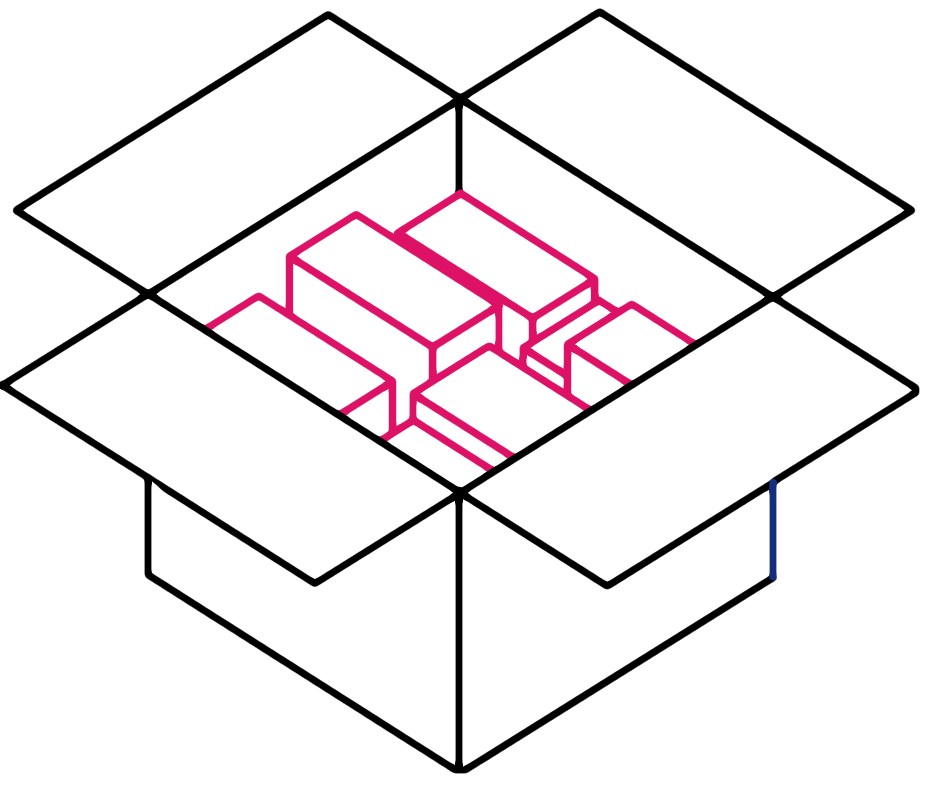
\includegraphics[width=1.6in]{assets/images/medieninformatikIcon.png}
\end{figure}

\vspace{0.4cm}

\begin{LARGE}
Bachelor thesis\\
\end{LARGE}
\vspace{0.4cm}

\begin{huge}
\textbf{\thesis}\\	
\end{huge}
\vspace{0.8cm}

\begin{LARGE}
\begin{normalsize}
prepared by\\ 
\end{normalsize}
\thisauthor\\
\end{LARGE}
\small Matriculation no.: 11118561 \\
\vspace{0.8cm}

\begin{Large}
\begin{normalsize}
presented at the\\
\end{normalsize}
TH Köln (University of Applied Sciences)\\
\begin{normalsize}
Gummersbach Campus\\
Faculty of Computer Science\\
and Engineering Science\\
\end{normalsize}
\end{Large}
\vspace{0.8cm}

\begin{Large}
\begin{normalsize}
in the study program\\ 
\end{normalsize}
\vspace{0.1cm}
Media Informatics\\
\end{Large}
\vspace{1.2cm}

\begin{tabular}{rl}
	Supervisor: &  Prof. Dr. Raphaela Groten\\
				&  Sven Kullack\\
				&  \small TH Köln (University of Applied Sciences) \\
\end{tabular}
\vspace{1.2cm}

\begin{normalsize}
Gummersbach, on February, 2023
\end{normalsize}

\end{center}

\end{titlepage}\newpage
%!TEX root = ../mai-joel_maximilian-bachelor_thesis.tex
%----------------------------------------------------------------------------------------
%	Debug options
%----------------------------------------------------------------------------------------
% chktex-file 12
% chktex-file 18
\thispagestyle{empty}

\begin{center}
\begin{tabular}{rl}
							&  \\[26.0em]
							
\large \textbf{Addresses:}	&  	\quad Joël Maximilian Mai\\
							&  	\quad Graf-Berghe-von-Trips-Ring 112\\
							&	\quad DE-50169 Kerpen\\
							&  	\quad joel\_maximilian.mai@smail.th-koeln.de\\[2.0em]
							
							&  	\quad Prof. Dr. Raphaela Groten\\
							&  	\quad TH Köln (University of Applied Sciences)\\
							&  	\quad Steinmüllerallee 6\\
							&	\quad DE-51643 Gummersbach\\
							&  	\quad raphaela.groten@th-koeln.de\\[2.0em]
							
							&  	\quad Sven Kullack\\
							&  	\quad TH Köln (University of Applied Sciences)\\
							&  	\quad Steinmüllerallee 6\\
							&	\quad DE-51643 Gummersbach\\
							&  	\quad sven.kullack@th-koeln.de\\[2.0em]
\end{tabular}
\end{center}\newpage

% Acknowledgements, keywords and abstract
%----------------------------------------------------------------------------------------
%	Debug options
%----------------------------------------------------------------------------------------
% chktex-file 2
% chktex-file 8
% chktex-file 11
% chktex-file 13
% chktex-file 18
% chktex-file 36
% chktex-file 39
% chktex-file 44
%----------------------------------------------------------------------------------------
\phantomsection%
%\addcontentsline{toc}{chapter}{Keywords}
\chapter*{Keywords}\label{cha:keywords}
\thiskeywords%

\begin{figure}[!h]
    \begin{center}
        \makebox[\textwidth]{
\includegraphics[width=\textwidth]{./assets/images/word-cloud-tagcrowd-greyscale.png}}
    \end{center}
\end{figure}

\phantomsection%
\addcontentsline{toc}{chapter}{Acknowledgements}
\section*{Acknowledgements}\label{cha:acknowledgements}
% In this part, you acknowledge any support you may have gotten while preparing your thesis.
% if an agency providing you with data, you definitely should thank them here
% It is also not uncommon to offer personal thanks to friends and/or family who supported the thesis
% You may also mention your adviser if she was helpful, but that is optional of course
First and foremost, I would like to express my deep gratitude to all those who have supported me throughout my academic journey, and especially during the completion of this thesis.

I am deeply thankful to my supervisor, Professor Dr.\ Raphaela Groten, for her unwavering support, guidance, and mentorship. Her expertise, encouragement, and constructive criticism were invaluable, and her belief in my abilities was a constant source of motivation.

I would also like to extend my appreciation to Sven Kullack for his inspiring discussions, which have shaped my academic and personal growth in countless ways.

I would also like to thank my family and friends for their unwavering love, support, and encouragement throughout this journey. Their belief in me was a constant source of strength, and I could not have completed this thesis without their patience and support.

Finally, I would like to express my gratitude to Jörg Beck, Timo Lauschner, Mario Hirschfeld, Michael Spiller, Normen Möller, Sonja Zuckerstätter, Norman Günther and Jean-Pierre Berchez. Their generosity and support were crucial to the completion of this work, and I am grateful for their contribution to my academic success.

In conclusion, I would like to acknowledge and express my appreciation to all the people who have made this thesis work possible. Their support and encouragement have been an immense source of strength and inspiration, and I am deeply grateful for the impact they have had on my academic and personal success.
\newpage
%----------------------------------------------------------------------------------------
%	Debug options
%----------------------------------------------------------------------------------------
% chktex-file 2
% chktex-file 8
% chktex-file 11
% chktex-file 13
% chktex-file 18
% chktex-file 36
% chktex-file 39
% chktex-file 44
%----------------------------------------------------------------------------------------
\phantomsection%
\addcontentsline{toc}{chapter}{Abstract}
\section*{Abstract}\label{cha:abstract}
% write all non-standard abbreviations in their entirety on their first appearance both in abstracts and papers themselves
% The summary is provided in the abstract of the beginning of your thesis
% Introduction: Brief overview of the purpose and significance of the research.
\textbf{Motivation: }Investigating the deviations from Scrum in theory and understanding their origins, helps future
practitioners to avoid derived issues and advancing the framework.\newline
% Background: Context and background information relevant to the research topic.
\textbf{Background: }The theory-practice gap of Scrum refers therefore to the difference between the principles, values, and practices prescribed by the Scrum Guide and the way it is implemented in real-world settings. Previous studies have provided insights into the strategies used by organizations and practitioners to overcome the challenges faced in implementing Scrum effectively.\newline
% Objectives: Clear statement of the research goals and objectives.
\textbf{Objectives: }The main objectives of this study are to provide common knowledge about Scrum and the theory-practice gap, identify the challenges faced by Scrum practitioners, investigate the impact of the theory-practice gap on organizations and teams and provide guidelines for organizations to improve their implementation of Scrum.\newline
% Methods: Description of the research design and methodology used.
\textbf{Method: }To ensure the validity of the various reasons and potential solutions for the theory-practice gap from the literature and bridge the gap, the evaluation of practitioners is essential. This provides insights into why individuals use Scrum, the challenges they face, and best practices for practitioners.\newline
% Results: Summary of the findings and outcomes of the research. Interpretation of the results and their significance to the field of study.
\textbf{Results: }This study found that small to medium size enterprises are more successful and adaptive to new methodologies, due to them reporting the least problems (8 out of 38 problems) and most benefits (6 out of 8 benefits). In addition, it was confirmed that commitment to the change in culture was uneved distributed to the departments, since only 50\% of the project management department and 25\% of the UI and UX department additionally utilized Scrum. The critical role of management in the adoption of Scrum was confirmed since the data collection stated that only 29\% had management support in writing, 14\% of middle management had learned new tasks and relinquished control and 28.6\% of the respondents stated that their management got in the way of their Scrum adoption. Furthermore, the study also found that organizations heavily rely on external experts, since since 33.33\% of the transformations were accompanied by Agile coaches and less than 25\% were executed solely by the team.
With 35\% of the teams reporting having received some form of training, this implies the need for more internal training. The level of testing and collaboration with clients was lower than expected since 29\% of the respondents reported not using demos and product increments for customer and client testing.\newline
% Conclusion: A brief summary of the main points and contribution of the research.
\textbf{Conclusion: }To summarize, organizations must prioritize the needs of their employees first. After that, they should research available methodologies and frameworks, invest in employee training, involve employees in the decision-making process, get the support of top management, and if needed Agile Coaches can provide valuable guidance in this regard. It is recommended to first establish a strong foundation in Agile principles before exploring scaling frameworks and adapting them to fit the specific needs of the organization, thereby keeping the methodology simple and avoiding complexity, ensuring the effectiveness of the scaling process.\newpage

% Table of contents
\phantomsection%
\addcontentsline{toc}{chapter}{Table of contents}
\tableofcontents
\newpage
\setcounter{page}{1}

%	Main
\pagenumbering{arabic}
%----------------------------------------------------------------------------------------
%	Debug options
%----------------------------------------------------------------------------------------
% chktex-file 2
% chktex-file 8
% chktex-file 11
% chktex-file 13
% chktex-file 18
% chktex-file 36
% chktex-file 39
% chktex-file 44
%----------------------------------------------------------------------------------------
\chapter{Introduction}\label{cha:Introduction}
% # Why does this section matter?
% # How does it reflect on investigating the gap in Scrum
% # Transition to the next section
Scrum has increasingly become the most used (61\%) \gls{framework} for \acf{asd}~\cite{Flynn20221AS} and other related fields. Despite its widespread \gls{adoption}, there is evidence of a gap between the theory and practice of Scrum, with many practitioners encountering challenges in implementing the \gls{methodology} effectively~\cite[p.~185]{Jilani2020ItG}.

The purpose of this thesis is to investigate this gap by analyzing problems and common solutions in literature and comparing them against the perceptions of Scrum practitioners. This study will provide a deeper understanding of the factors that contribute to the theory-practice gap of Scrum and how practitioners are addressing these challenges. 

The intended audience for this thesis comprises organizations that are in the process of adopting, have already adopted, or are planning to adopt the Scrum \gls{framework}. This includes individuals in various roles, such as developers, managers, and other relevant positions who have an interest in utilizing Scrum as a \gls{methodology}.

The results of this study will contribute to the body of knowledge on the theory-practice gap of Scrum and provide insights for organizations and practitioners to improve their implementation of the \gls{methodology}.

\section{Definition of the theory-practice gap of Scrum}\label{sec:DefinitionTheoryPracticeGap}
% What is a theory-practice gap
\citeA[p.~2]{Greenway2019Wia} explain that the root cause for a gap between theory and practice is commonly at the communicational level. \citeA{Carr1980TGb} adds that the jargon of the theory is too difficult or too abstract to understand. Another cause for a gap between theory and practice occurs when theoretical procedures are no longer suitable for a situation~\cite[pp.~61--76]{Carr1980TGb}.

% What is the theory-practice gap of Scrum
The theory-practice gap of Scrum refers therefore to the difference between the \glspl{principle}, values, and practices prescribed by the Scrum Guide and the way it is implemented in real-world settings.

% Reasons for a gap in Scrum
The gap exists due to a variety of factors such as inadequate training~\cite[p.~72]{Maximini2018ISi}, lack of understanding of the \gls{methodology}, cultural differences~\cite[pp.~27]{Koning2019AT}, and resistance to change~\cite[pp.~37--38]{Boehm2005Mct}.

\section{Importance of investigating the theory-practice gap of Scrum}\label{sec:ImportanceOfInvestigating}
Investigating the theory-practice gap of Scrum is important for several reasons. 

% understanding the challenges faced by the practitioners 
Firstly, due to Scrum's wide \gls{adoption}, understanding the challenges faced by the practitioners leads to possibilities to improve the \gls{methodology} of Scrum. But it is important to not only focus on the literature but to fact-check the results by actual practitioners.

% the theory-practice gap of Scrum can lead to reduced benefits
Secondly, the theory-practice gap of Scrum can lead to reduced benefits due to deviations from the recommended \glspl{method} and culture. Investigating those deviations and understanding their origins, may help future practitioners to avoid them.

% understanding the factors that contribute to the theory-practice gap of Scrum 
Thirdly, understanding the factors that contribute to the theory-practice gap of Scrum may not only help the practitioners of Scrum but the ones that want to build upon it and advance it.

Moreover, the results of this study can be used by organizations and teams to identify areas for improvement in their implementation of Scrum and to develop strategies to overcome the challenges faced in implementing the \gls{methodology} effectively.

\section{State of the Art}\label{sec:StateOfTheArt}
% Challenges
Previous studies have investigated the challenges faced by Scrum practitioners in implementing the \gls{methodology} effectively and the factors that contribute to the gap. These studies have identified a range of challenges, including removing resistance to the change~\cite[pp.~37--38]{Boehm2005Mct}, establishing the right amount of control~\cite[p.~4]{Verwijs2021Ato}, incorporating the client~\cite[p.~5]{Coyle2009Acs}, transitioning from \gls{plan-driven} roles~\cite[p.~16]{Moreira2013AtA}, scaling Scrum for larger organizations~\cite[pp.~124--126]{Maximini2018ISi}, establishing a common culture~\cite[p.~4]{Barroca2019Ata}.

% Impacts
Additionally, previous studies have explored the impact of the theory-practice gap on organizations and teams, such as decreased effectiveness due to handovers between departments~\cite[p.~119]{Vilkki2010Wai}, frustration due to frequent intervening of management~\cite[p.~29]{Koning2019AT}, incomplete \glspl{transition} to Scrum due to limited expertise and control given to Scrum Masters.

% Solutions
These studies have also provided insights into the strategies used by organizations and practitioners to overcome the challenges faced in implementing Scrum effectively. These studies have found that hiring external consultants~\cite[p.~77]{Moreira2013AtA}, intensive training of employees~\cite[p.~72]{Maximini2018ISi}, a planned approach to the \gls{transition}~\cite[p.~37]{Thorgren2019Tro} and regular analysis of the status of the \gls{transition}~\cite[p.~395]{Rubin2012ESA} help overcome the challenges faced in implementing Scrum effectively. 

The current state of the art on the theory-practice gap of Scrum highlights the importance of investigating this gap and provides a foundation for further research in this area.

\section{Overview of the research question and objectives}\label{sec:OverviewResearchQuestion}
This research aims to investigate the theory-practice gap of Scrum and to provide insights into the perceptions of Scrum practitioners. The research questions guiding this study are: 

What is the theory-practice gap of Scrum, what are its characteristics, what are the perceptions of Scrum practitioners regarding the challenges faced, what were their solutions tried and what \glspl{guideline} can be derived from them?

Therefore, the objectives of this study are to:
\begin{itemize}
    \item Provide common knowledge about Scrum and the theory-practice gap
    \item Identify the challenges faced by Scrum practitioners
    \item Investigate the impact of the theory-practice gap on organizations and teams
    \item Explore the perceptions of Scrum practitioners
    \item Provide insights for organizations and practitioners to improve their implementation of Scrum
\end{itemize}

\section{Structure of the Thesis}\label{sec:StructureThesis}
The thesis is organized into several chapters that address different aspects of the research questions and objectives. The structure of the thesis is as follows:

\begin{description}[style=nextline]
    \item[Chapter \ref{cha:Introduction}: Introduction]
    This chapter provides a general definition of the theory-practice gap of Scrum, the significance of this thesis, the research questions and objectives, and the structure of the thesis.
    \item[Chapter \ref{cha:LiteratureReview}: Literature Review]
    This chapter reviews the existing body of knowledge on Scrum, and the theory-practice gap of Scrum, including previous studies, theories and strategies to overcome the gap. It also provides the first synthesis of the findings.
    \item[Chapter \ref{cha:Method}: Method]
    This chapter outlines the research design, the methods used to collect and analyze data, and the procedures for data analysis.
    \item[Chapter \ref{cha:Discussion}: Discussion]
    This chapter presents the results of the study and discusses them in relation to the findings from the literature and ties them back to the research questions.
    \item[Chapter \ref{cha:Conclusion}: Conclusion]
    This chapter provides a summary of the main findings of the study, the conclusions drawn from the results, and the implications of the study for organizations and practitioners but it also states the limitations of the study.
    \item[Appendix]
    This appendix includes used acronyms, glossary entries, a list of participants wishing to be named, the questionnaire as well as the results and any additional information that supports the main body of the thesis.
\end{description}
%----------------------------------------------------------------------------------------
%	Debug options
%----------------------------------------------------------------------------------------
% chktex-file 2
% chktex-file 8
% chktex-file 11
% chktex-file 13
% chktex-file 18
% chktex-file 36
% chktex-file 39
% chktex-file 44
%----------------------------------------------------------------------------------------
\chapter{Literature Review}\label{cha:LiteratureReview}
% # Why does this section matter?
% # How does it reflect on investigating the gap in Scrum
% # Transition to the next section
% What literature offers about the gap (Problems -> Solutions)
The literature review forms an important part of this thesis as it provides a comprehensive understanding of the existing body of knowledge on the theory-practice gap of Scrum. This chapter aims to identify and critically review previous studies, theories, and strategies related to the research questions and objectives. The literature review will provide a foundation for the research by highlighting the gaps in the existing knowledge and identifying areas that need further investigation.

The purpose of this chapter is to:

\begin{itemize}
    \item Provide an overview of Scrum methodology
    \item Explain the theory-practice gap of Scrum
    \item Identify the key theories, strategies, and studies related to the research questions and objectives
    \item Evaluate the strengths and limitations of previous research on the theory-practice gap of Scrum
    \item Identify the gaps in the existing body of knowledge that need further investigation
\end{itemize}

The literature review will be organized into sections based on the key themes and concepts that emerged from the review of the literature. This will provide a structured overview of the existing body of knowledge and highlight the key findings of previous research on the theory-practice gap of Scrum.

\section{Overview of the Scrum framework}\label{sec:OverviewScrumMethodology}
Scrum is a widely adopted \gls{framework} for Software Development and project management. As a \gls{framework}, Scrum was once only the \gls{methodology} of a few organizations and over time became a \gls{framework}. In \citeA[p.~3]{Schwaber2020Tsg} own words: "Scrum is a lightweight \gls{framework} that helps people, teams and organizations generate value through adaptive solutions for complex problems." The Scrum \gls{framework} is designed to help teams achieve their goals through a series of iterations and continuous improvement.

This section provides an overview of the Scrum \gls{methodology} by describing the origins, roles, events and artifacts that are part of Scrum and how they contribute to the success of the project.

% origins of Scrum
While originally invented by \citeA{Takeuchi1986TNN}, Scrum was first implemented as a \gls{framework} at the Easel Corporation and then first publicly presented in 1995 by Ken Schwaber and Jeff Sutherland at the Object-Oriented Programming, Systems, Languages and Applications (OOPSLA) Conference '95 in Austin, Texas. The name for the \gls{framework} stems from rugby, where it describes a formation of players. Today Scrum implies teamwork and collaboration as well as coordination. The first publication of the Scrum Guide was in the year 2010 as an effort to clarify what Scrum is and what it is not. The Scrum Guide refined on several occasions since~\cite{Kneafsey2015ASH}.

% what Scrum is now
The official Scrum Guide only serves the barebone explanation to incorporate Scrum in theory. It utilizes its abstractness to be more versatile. Rather than being a fixed process, accompanied by extensive documentation, it provides a set of \glspl{guideline} for the implemented interactions and relationships between roles.
Although trying to be abstract and versatile, the Scrum Guide also warns about changing the core design of Scrum by leaving out elements or ignoring the set rules of Scrum. By doing so a company does risk rendering the process useless or potentially even doing damage. An iterative and incremental approach in Scrum is used to optimize predictability and enhance the control of risk~\cite{Schwaber2020Tsg}.

% roles of Scrum
For Scrum to work, groups of people with all needed skills and expertise are needed to do or share the work between them. Responsible for all product-related activities from stakeholder collaboration, verification, maintenance, operation, experimentation, research and development, and anything else that might be required is the Scrum Team composed of Developers, a Scrum Master and a Product Owner~\cite[p.~5]{Schwaber2020Tsg}. Their definitions and responsibilities are as follows:

\begin{description}[style=nextline]
    \item[Developers]
    The Scrum Guide defines "\glspl{developer}" as encompassing all individuals involved in the development process, including architects and designers~\cite[p.~1]{Schwaber2020Tsg}. The Scrum team composition can be adjusted as required to meet the objectives of each sprint~\cite[p.~203]{Rubin2012ESA}. The Scrum approach prioritizes collaboration and cross-functional teams, giving the Scrum team the knowledge and expertise necessary to build the product increment, thereby reducing the risk of information loss compared to a \gls{plan-driven} approach. The diversity of skills and expertise among Scrum team members allows for the collective utilization of knowledge, leading to the creation of a thoughtful and valuable product.
    \item[Product Owner]
    The role of the \ac{po} is to optimize the value of the product and carry out various duties, including defining the product goal, establishing the product backlog with priorities, and responding to inquiries~\cite[pp.~5--6]{Schwaber2020Tsg}. The ideal \ac{po} should be the sole authoritative source with knowledge of the domain and comprehension of the needs of \glspl{client} and \glspl{customer}. To minimize confusion within the Scrum Team, it is recommended to appoint a single \ac{po} instead of a committee. However, in some organizations, an excessive workload may necessitate the division of responsibilities among multiple individuals, potentially reducing the capability of a single \ac{po} to effectively fulfill their responsibilities~\cite[p.~182]{Rubin2012ESA}.
    \item[Scrum Master]
    The role of the Scrum Master is crucial in facilitating the implementation of the Scrum \gls{framework}, not only in terms of theoretical understanding but also in terms of practical application. As specified in the Scrum Guide, the Scrum Master has the responsibility of promoting the \gls{adoption} of Scrum across the entire organization. The extent to which the Scrum Master can successfully integrate the Scrum \gls{framework} into the organization is dependent on the level of authority and influence they are granted by the organization~\cite[p.~6]{Schwaber2020Tsg}.
\end{description}

% events of Scrum
The Scrum \gls{framework} utilizes specific events during a sprint to raise transparency, inspection and adaption~\cite[p.~3]{Schwaber2020Tsg}. These events are as follows:

\begin{description}[style=nextline]
    \item[Sprint]
    The Sprint, as defined by the Scrum Guide, is a time-bound event that encompasses all other events in the \gls{framework}. During a Sprint, changes that would jeopardize the achievement of the Sprint Goal are not allowed. The Product Backlog may be continuously refined and its scope clarified and renegotiated with the \ac{po}. Sprints offer the advantage of synchronizing work with other teams, promoting collaboration and reducing the waste of time and effort on non-value-adding tasks. This protected \gls{framework} increases the reliability of the system towards stakeholders and enhances the ability of all parties to plan and coordinate effectively.~\cite[pp.~7--8]{Schwaber2020Tsg}
    \item[Sprint Planning]
    The Sprint Planning event involves the participation of all Scrum Team members to define a shared understanding of the work results to be delivered, referred to as the Sprint Goal. This event promotes clarity and reduces misunderstandings by defining the purpose, scope, and approach of the work to be executed in the upcoming Sprint. By planning and defining what should and should not be done during the Sprint, supported by the experts of the team, this event helps to minimize the impact of changing requirements and distractions from non-critical tasks, resulting in more efficient use of time and resources.~\cite[p.~8]{Schwaber2020Tsg}
    \item[Daily Scrum]
    The Daily Scrum is a collaborative event aimed at inspecting the progress towards the Sprint Goal and adapting the Sprint Backlog. This process facilitates mutual assistance and makes team barriers visible, reducing the need for multiple meetings and allowing for longer periods of focused work. As a result, the quality of the product is improved. The Daily Scrum is not designed for management control, but rather for team collaboration and progress monitoring.~\cite[p.~9]{Schwaber2020Tsg}
    \item[Sprint Review]  
    The Sprint Review serves as a platform for the Scrum Team to demonstrate and assess their progress toward the Product Goal with stakeholders. Through this interactive session, the team can identify dependencies and make necessary adjustments to the Product Backlog. The Sprint Review should not be considered a presentation, but rather a collaborative working session.~\cite[p.~9]{Schwaber2020Tsg}
    \item[Sprint Retrospective] 
    During a Sprint Retrospective, the Scrum Team engages in a collaborative examination of their process and performance with the aim of identifying and implementing improvements. Moderated by the Scrum Master, the team focuses on the interactions, processes, tools, and individuals involved, rather than the specific work results. The outcome of the Sprint Retrospective is an increased level of awareness, effectiveness, and reduced potential for conflict and frustration within the team.~\cite[p.~10]{Schwaber2020Tsg}
\end{description}

% artifacts of Scrum
The Scrum \gls{framework} defines three primary artifacts in order to manage the workload:

\begin{description}[style=nextline]
    \item[Product Backlog]
    The Product Backlog is a prioritized list of items that describe the functional and non-functional requirements of the product, including features, enhancements, and bug fixes. The list is continually refined and updated based on the Product Goal, and is never considered to be a comprehensive or final representation of the product's requirements. The prioritization of the items in the Product Backlog is determined by the \ac{po} and represents their understanding of the relative importance of the items in achieving the Product Goal.~\cite[pp.~10--11]{Schwaber2020Tsg}
    \item[Sprint Backlog]
    The Sprint Backlog is a dynamic list of items compiled by the development team that outlines the work they have committed to completing during a specific Sprint. It is subject to change and \gls{adaptation} as the Sprint progresses and is maintained exclusively by the development team. The amount of detail it holds has to be sufficient to inspect the progress towards the Sprint Goal~\cite[p.~11]{Schwaber2020Tsg}
    \item[Increment]
    The Increment is a critical component, serving as a tangible representation of progress towards the Product Goal. It is created through the addition of work items that have been verified to meet the \gls{dod}, ensuring that each Increment is usable and integrates seamlessly with prior Increments. The creation of multiple Increments within a Sprint is supported by empiricism, and their sum is presented at the Sprint Review. It is important to note that work cannot be considered part of an Increment unless it has met the established \gls{dod}.~\cite[pp.~11--12]{Schwaber2020Tsg}
\end{description}

% Agile Software Development
Although never stated in the Scrum Guide directly, the \gls{methodology} of Scrum overlaps with the one of \acf{asd} and could be viewed as a practical application of \ac{asd}. That said, Scrum could be implemented without the integration of the \ac{asd} \gls{mindset}~\cite[p.~56]{Moreira2013FoA}, although the organization would probably not benefit as much from Scrum~(\citeNP[p.~123]{Moreira2013AtA};~\citeNP[pp.~7--9]{Bannink2014Cit}). The goal of \ac{asd} is to deliver working software to \glspl{client}, while still considering sustainability and clear documentation. Despite the lack of explicit planning and risk management in the \ac{agile-manifesto}, the approach is not inherently riskier~\cite[p.~3]{battoia2019innovation}. Instead, it prioritizes collaboration with \glspl{client} and values their role in the project's success. The use of incremental payments and sprints helps mitigate the risk of scope creep, while also allowing for a more flexible and adaptive design process in response to changes~\cite{Beck2001MfA}.

\quotethis{Agile:\newline
Work small, Talk to each other, Make people’s lives better\newline
That's it. All that other junk is a distraction.}{\citeNP{AllenHolub2022AW}}

\newpage
\takeaways{
    In this section, the fundamental \glspl{principle} of the Scrum \gls{methodology} and its key components were presented as a foundation for the exploration of the theory-practice gap of Scrum. Scrum is a \gls{framework} that originated from a functional \gls{methodology}, meaning its \glspl{method} have been tested and applied within teams. However, the efficacy of the \gls{methodology} is contingent on its compatibility with a particular team. Although Scrum can be utilized without the \ac{asd} mindset, this is unlikely to lead to optimal results as Scrum is rooted in the \gls{agile} \gls{methodology}. Hence, both the \gls{ideology} of \ac{asd} and the \gls{methodology} of Scrum are necessary for Scrum to function effectively. It is important to note that adopting Scrum does not automatically translate to being \gls{agile}. Additionally, the \gls{agile} approach is not inherently riskier than traditional waterfall processes as the \gls{client} retains control throughout the project and can decide to discontinue the project at any time while still retaining a usable product concept.
}

\section{Explanation of the theory-practice gap of Scrum}\label{sec:ExplanationGapScrum}
% Summary and goals for the section
% Why it is important for the research question
% What this section will add to the thesis
This section aims to clarify the concept of the theory-practice gap of Scrum by providing clear definitions of the terms "theory" and "practice". The distinction between "theory" and "ideology" will also be discussed. A comprehensive overview of the general theory-practice gap will be presented, including its common dimensions and forms. Lastly, a characterization of the specific theory-practice gap within the context of Scrum will be provided. The resulting frame will be the foundation for the contribution of this thesis.

% What is "theory"
According to the theorization by \citeA{Wacker1998Ado}, theory serves as an abstraction of a portion of reality, aimed at providing explanatory insights into the pragmatic world. \citeA{Carr1980TGb} further elaborates that theory and practice are not inherently linked, but rather theory influences practice through a critical and rational analysis that assesses and justifies the practices, leading to the evolution and \gls{transformation} of the way in which practice is understood and experienced. This process can also be observed in the development and refinement of the Scrum Guide. For a more in-depth definition of theory, the research done by \citeA{Moustafa2014DoT} is recommended.

% What is the difference between "theory" and "ideology"
The difference between theory and \gls{ideology} can be best understood by examining the \gls{mindset} of individuals. A \gls{mindset} is a cognitive orientation, characterized by patterns of thoughts, attitudes and beliefs towards reality and the self. It is often established as a habit~\cite{Dictionary2022ME, 2018IvM}. When individuals share a common set of beliefs, they form a collective ideology, which encompasses a doctrine, philosophy, or set of values informed by underlying \glspl{principle}~\cite{Dictionary2022IE, 2018IvM}. In contrast, theory aims to provide explanations, descriptions, and predictions of interactions and behaviors~(\citeNP[pp.~361--363]{Wacker1998Ado};~\citeNP{Dictionary2022TE}). For a more in-depth definition of ideology, the research done by \citeA{Moramollu2016Ial} is recommended.

The distinctiveness of theory and \gls{ideology} is depicted in Figure~\ref{fig:theory-ideology}.

\newpage
\begin{figure}[!h]
	\begin{center}
        \makebox[\textwidth]{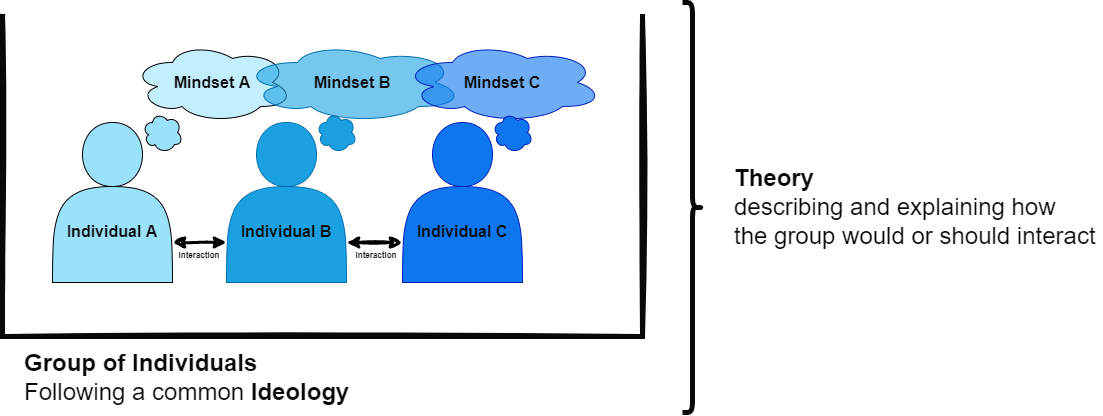
\includegraphics[width=\textwidth]{./assets/images/ideology-mindset-theory.png}}
        \caption{Visualization of the interaction between ideology and theory}\label{fig:theory-ideology}
    \end{center}
\end{figure}

% What is "practice"
\citeA[pp.~3--5]{Wenger1998Cop} posit that there exist various types of groups for practices, each of which can be at a different stage of development, ranging from the formation of a community to its eventual dissolution. The choice of Scrum as a \gls{framework} and \ac{asd} as a \gls{mindset} can vary, with the success of these choices being contingent on the nature of the group. According to \citeA[p.~5]{Wenger1998Cop}, communities can have five different relationships with organizations, with those that are unrecognized or bootlegged not contributing to organizational \gls{transformation} due to a lack of maturity and size. On the other hand, a community that is legitimized, seen as strategic, or transformative can have a significant impact and receive support from the organization it aims to transform or improve.

% What is a gap in theory and practice
The theory-practice gap is a long-debated concept among scientifically oriented philosophers, who question the practical implications of theories~\cite[p.~61]{Carr1980TGb}. According to \citeA[p.~2]{Greenway2019Wia}, while there are various unclear definitions of a theory-practice gap, research into it is often aimed at improving communication between the two. \citeA[p.~60; p.~65]{Carr1980TGb} cites the difficult jargon of theories as a possible reason for the gap, as well as differences in language and evaluation criteria between theorists and practitioners. \citeA[p.~63]{Carr1980TGb} suggests that the gap often arises from methodological problems and can be solved by changing the \gls{methodology} through new insights from practitioners. He also writes that the theory-practice gap can only be closed by involving practitioners in the solution development process, rather than relying solely on theorization and \glspl{guideline}. An integrated or problem-based approach is unlikely to lead to satisfactory results. The active participation of practitioners is essential in enhancing the theoretical field.~\cite[p.~67]{Carr1980TGb}

% What Attributes does it take on
The theory-practice gap can therefore be characterized in three dimensions: language, evolution, and \gls{methodology}. The language dimension refers to the cause of the gap due to specialized jargon in theory or lack of understanding in practice. The \gls{methodology} dimension highlights the causes of the gap between theory and practice through the theory not being derived from the actual practices of practitioners, not being suited for the activities faced by practitioners, or evaluating success differently. The evolution dimension illustrates the cause of the gap due to the theory lagging behind advancements in practice.

The dimensions and attributes of a general theory-practice gap derived from the previous paragraphs are visualized in Figure~\ref{fig:gap-attributes}

\begin{figure}[!ht]
	\begin{center}
        \makebox[\textwidth]{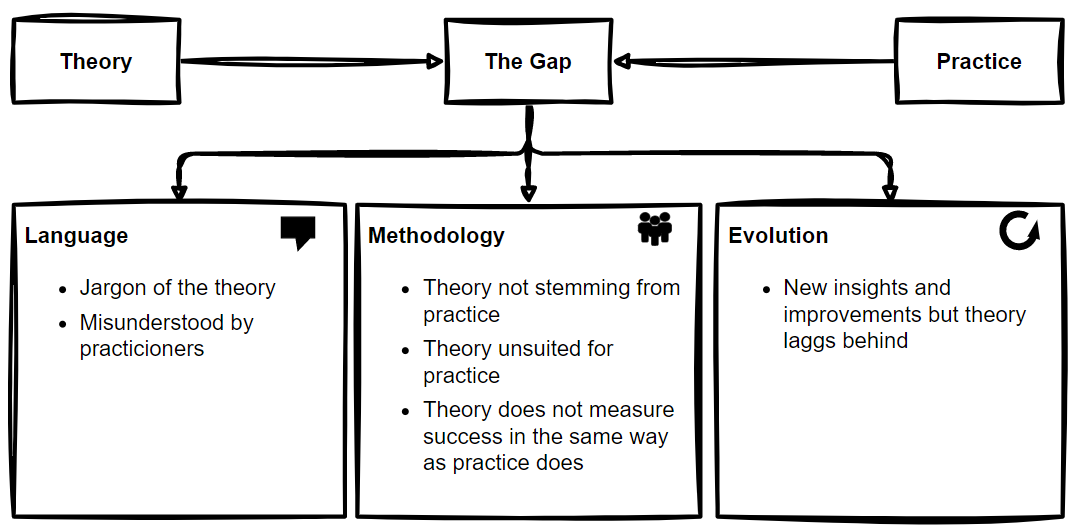
\includegraphics[width=\textwidth]{./assets/images/attributes-dimensions-gap.png}}
        \caption{A general theory-practice gap and its attributes and dimensions derived from Carr's description}\label{fig:gap-attributes}
    \end{center}
\end{figure}

% What Attributes does the gap of Scrum take on
Utilizing the model for a general gap in theory and practice, the gap in the context of Scrum can be attributed as follows:

The first dimension, Language, is characterized by specialized jargon in the theory of Scrum, as well as misunderstandings and misconceptions about Scrum's \glspl{method}. The abstractness of the Scrum Guide, as an example, could therefore lead to discussions about who is meant by the role \glspl{developer}, since the common association with this role are programmers. This can lead to questions about the effectiveness of Scrum since a misunderstanding regarding the role of the \gls{developer} could lead to arguments such as Scrum lacking upfront design. The lack of clear verbalization of risk management in the Scrum Guide is another example of a possibility of miscommunication, since some may argue that missing risk management leads to riskier projects. 

The second dimension, \Gls{methodology}, is the largest of the gap and is characterized by difficulties in transforming or merging existing \glspl{methodology}, roles or control structures, budgeting training, and scaling self-management and self-organization to larger teams. A common problem with the \gls{transition} from a \gls{plan-driven} process to Scrum can be the \gls{transformation} of management roles since in Scrum, managers no longer micromanage but instead become servant leaders.

The third dimension, Evolution, is characterized by the challenge of scaling Scrum beyond the initial idea of small \gls{self-managing} teams and single projects and finding a \gls{framework} that enables teams of teams to deal with multiple projects at the same time. An example of this could be the divergence of the \glspl{framework} for scaling Scrum. Some stay true to the \gls{agile} \gls{ideology} while some reintroduce command-and-control structures.

These examples illustrate how the theory-practice gap can lead to Scrum being less effective than it was intended to be and highlight the importance of continuously revisiting and adjusting the way Scrum is being implemented to ensure that it aligns with the underlying \glspl{principle} and values of the \gls{framework}.\newline
The derived model for Scrum's gap of theory and practice is visualized by Figure~\ref{fig:gap-attributes-scrum}.

\begin{figure}[!ht]
	\begin{center}
        \makebox[\textwidth]{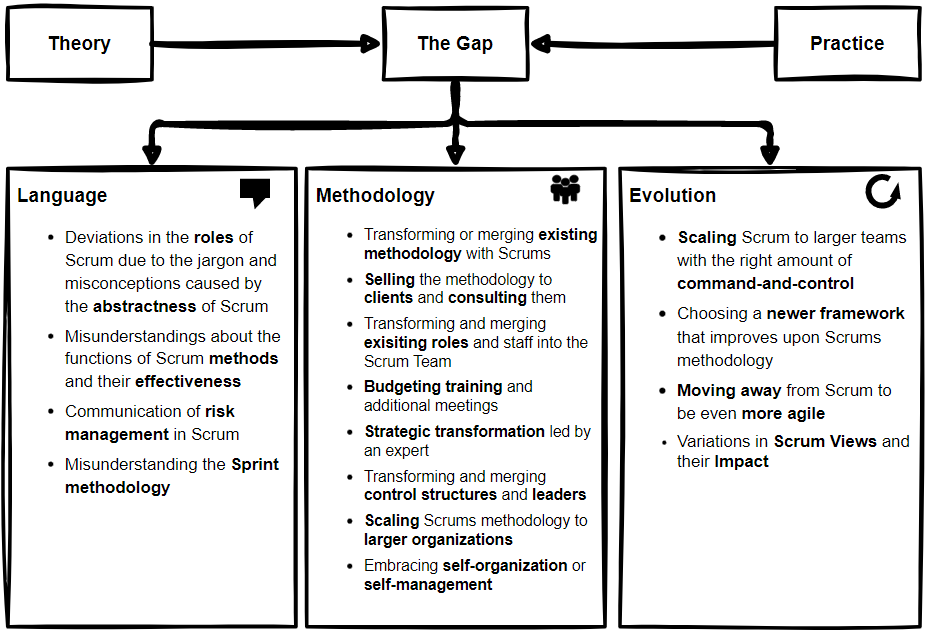
\includegraphics[width=\textwidth]{./assets/images/attributes-dimensions-gap-scrum.png}}
        \caption{The theory-practice gap of Scrum and its attributes and dimensions}\label{fig:gap-attributes-scrum}
    \end{center}
\end{figure}

\takeaways{
    The gap between theory and practice in Scrum can be defined as the difference between the concepts and models presented in Scrum literature and the actual implementation and application of these concepts in real-world scenarios. The theory-practice gap can be divided into three dimensions: language, \gls{methodology}, and evolution. Previous studies have shown that effective communication and bridging the gap can be achieved through the development of practical solutions by practitioners, rather than relying solely on theory and \glspl{guideline}. The Scrum gap has several attributes including deviations in roles due to misunderstandings in the abstract Scrum Guide, perceived higher risk compared to traditional development \glspl{method}, the ineffective merging of traditional \glspl{methodology} with the Scrum framework, lack of expert-guided \gls{transformation} planning, difficulties in embracing self-organization and self-management, and scaling challenges due to the addition of command-and-control structures and the selection of inappropriate \glspl{framework}.
}

\newpage

\section{Previous studies on the theory-practice gap of Scrum}\label{sec:PreviousStudies}
% # Identify the key theories, strategies, and studies related to the research questions and objectives
% # Evaluate the strengths and limitations of previous research on the theory-practice gap of Scrum
% Purpose of the section
% Significance of examining previous studies
Previous studies on the theory-practice gap of Scrum have explored the reasons for this disparity, focusing on various factors such as misunderstandings, lack of training, and difficulty in scaling Scrum to larger organizations. This section aims to provide a comprehensive review of these previous studies, highlighting key findings and offering insights into the current state of knowledge on the theory-practice gap of Scrum. By doing so, this section will lay the foundation for a deeper understanding of the challenges and opportunities associated with bridging the gap between Scrum theory and practice.

% Overview of previous studies
% Theoretical foundations of previous studies
\subsection*{Historical evolution of Scrum}\label{subsec:historyOfScrum}
The historical evolution of Scrum can be traced back to its origins in the mid-1990s when Ken Schwaber and Jeff Sutherland developed the Scrum \gls{framework}. They have tested the Scrum \gls{methodology} in some organizations and found it to be valuable.

With the first iterations of the Scrum Guide clarifying what Scrum is and introducing flexibility to the \gls{framework} in order to be widely adoptable, it visualizes the increasing interest in developing in a more \gls{agile} manner. But with the broader interest may have come some misconceptions about the values and \gls{methodology}, which led to the introduction of the key values and an emphasis of transparency. The events of Scrum, for example, the Daily Scrum, had been specified and artifacts and their handling described.~\cite[Revision 2010--2013]{Schwaber2020SGR}

Scrum's success had led to the development of \glspl{framework} encompassing Scrum's \gls{methodology} or parts of it and being targeted at more specific demographics, for example, scaling \glspl{framework} such as the \ac{safe} and \ac{less}. This may have led to the Scrum Guide clarifying that Scrum in essence is still made for smaller teams. They enforced the meaning of servant-leaders and the role of the Scrum Master accordingly. In addition, they emphasized the benefits of working in small teams and explained that they could be kept by having networks of small teams and avoiding introducing command-and-control structures.~\cite[Revision 2013--2017]{Schwaber2020SGR}

In the latest revisions, Scrum has been reduced to being a minimally sufficient framework, with an emphasis on a small team working together, the Scrum Team. It was described that way because the authors of the Scrum Guide wanted to clarify, that the Scrum Team does collaborate closely and does not have frequent handovers like the former \gls{plan-driven} approaches had between departments. This revision also clarified the artifacts to make them easier understandable. In order to be understood by a wider audience, the Scrum Guide has been simplified in the language by eliminating redundant, complex statements and removing any remaining reference to IT. This is probably due to Scrum encompassing a wider range of domains and industries, including product development, healthcare, and education.~\cite[Revision 2017--2020]{Schwaber2020SGR}

Overall, the historical evolution of Scrum reflects the growing popularity and acceptance of the Scrum \gls{framework}, as well as the ongoing efforts to refine and improve its practices and outcomes.

% Explanation of relevant theories related to the theory-practice gap
% Summary of key findings from previous studies
% Comparison of previous studies in terms of research methodologies, sample populations, and outcomes
% Overview of how previous studies have applied these theories to Scrum
\subsection*{Summary of key findings from previous studies}
In the field of Scrum, numerous studies have been conducted over the years to uncover its various aspects, benefits, and limitations. This body of research has helped to establish Scrum as a popular \gls{framework} for \ac{asd} and provided insight into its implementation and use in organizations. This section will provide a summary of the key findings from previous studies that have been conducted on Scrum. The objective of this summary is to provide a comprehensive understanding of the research that has been done in this field and highlight the key insights and trends that have emerged from these studies. These key findings will be sorted by their associated dimension and attribute derived from the Figure~\ref{fig:gap-attributes-scrum}.

\subsubsection*{Deviations in the roles of Scrum}\label{subsubsec:DeviationOfRoles}
The integration of Scrum as a \gls{methodology} can be problematic for some organizations, as indicated by \citeA[p.~1]{Diebold2015Wdp} who found that only one-fourth of organizations using Scrum followed the \glspl{guideline} set forth in the Scrum Guide. Misunderstandings of roles within the team can lead to frustration, as stated by \citeA[p.~29]{Koning2019AT}. Even though the Scrum Guide defines anyone who feels included as a \gls{developer}, additional roles such as \ac{ux} designer get added to the Team. Organizations often turn to external experts to aid in the integration of Scrum~(\citeNP[p.~5]{Bannink2014Cit};~\citeNP[p.~2]{Sidky2007ADA}). This raises questions about the effectiveness of certified Scrum Masters in actually executing the integration and training process. On the other hand, organizations utilizing scaling \glspl{framework} for Scrum frequently utilize these external experts~(\citeNP[p.~1]{Paasivaara2016SSi};~\citeNP[p.~6999]{Moe2019Tai}). Further research is needed to confirm these conclusions, as the literature provides no clear answer.

\subsubsection*{Misunderstandings about the functions of Scrum methods and their effectiveness}\label{subsubsec:MisunderstandingsOfScrum}
\citeA[p.~3]{Reddy2021HMU} argue that Scrum does not put enough emphasis on conception, leading to potential refactoring. \citeA[p.~56]{Moreira2013FoA} acknowledges that Scrum can be integrated into a \gls{plan-driven} process. Scrum and \ac{asd} are different but often used together, leading to misinterpretation due to lack of understanding. Scrum provides \glspl{method} while \ac{asd} provides \gls{mindset} and values, but Scrum without \ac{asd} lacks the essence of its \gls{methodology}. New organizations may find the abstractness of Scrum definitions misleading. With valuable increments each Sprint, Scrum delivers more frequently than \gls{plan-driven} approaches~\cite[p.~34]{Rubin2012ESA}.

\subsubsection*{Communication of risk management in Scrum}\label{subsubsec:RiskManagementInScrum}
Risk management in \ac{asd} reduces the risk of developing a non-viable or non-desirable product through collaboration with the \gls{client} and planning each sprint~\cite[p.~18]{battoia2019innovation}. The \gls{client} benefits from frequent releases~\cite[p.~4]{RachevaCpi} and direct communication with the team, leading to faster feedback and reduced miscommunication~\cite[p.~193]{Cho2008IAC}. The \gls{transition} to an \gls{agile} approach requires the \gls{client} to understand their impact on prioritizing the backlog and the benefits of using use-cases and removing feedback loops~(\citeNP[p.~153]{mancl2019xp};~\citeNP[p.~36]{Boehm2005Mct}). 

This results in higher-quality products, increased \gls{adaptation} to changes, and improved \gls{customer} satisfaction~\cite[p.~99]{Abrahmson2002ASD}. Detecting problems early on and short communication channels between the team and \gls{client} lead to more efficient resolution of issues.

\subsubsection{Misunderstanding the sprint methodology}\label{subsubsec:UnderstandingSprints}
The Sprint \gls{methodology} is a fixed-length event of one month or less designed to achieve consistency in product development~\cite[p.~7]{Schwaber2020Tsg}. It is commonly utilized for achieving a specific goal, such as the Product Goal, but it is not limited to software development. Instead, it enables cross-functional teams to build functional increments that can be shared across teams. This approach offers several benefits.

The full application of the Sprint \gls{methodology} involves a \gls{client} contracting an organization to develop their product. A Concept Sprint can be used to test the waters and develop a product vision under the guidance of the \gls{client}. If the \gls{client} is satisfied with the work, they can continue with the development by paying for each subsequent sprint, which will deliver a functional and valuable increment prioritized by value. If the product reaches a fully functional state, the Scrum Team can use Enhancement Sprints to incorporate product backlog items that were not deemed important earlier~\cite[p.~2]{Sutherland2005Fos}.

The Sprint \gls{methodology} can also be applied within an organization through Integration Retrospectives and Enhancement Sprints to improve processes. This would enable organizations to reflect on their progress towards being more adaptive and \gls{agile} and how they can optimize their way of working, effectively treating their processes as a product they continuously develop and improve~\cite[pp.~395--396]{Rubin2012ESA}.

\subsubsection*{Transforming or merging exsisting methodology with Scrums}\label{subsubsec:TransformingTheMethodology}
Scrum is a \gls{methodology} that can be used by development departments but it can only reach its full potential if the entire organization embraces it~(\citeNP[p.~233]{Rubin2012ESA};~\citeNP[p.~15]{Maximini2018ISi}). According to the \citeA{20211AS}, the main challenge to adopting and expanding \gls{agile} practices is inconsistent processes and practices across teams.

\subsubsection*{Transforming and merging existing roles and staff into the Scrum Team}\label{subsubsec:TransformingRoles}
\citeA[p.~214]{Rubin2012ESA} argues that to fully realize the benefits of Scrum, the entire organization should embrace it and the \ac{asd} \gls{ideology}. For example, the role of \ac{ui} designer should be part of the Scrum Team to reduce communication time and allow for easier change management, but would be also described as a \gls{developer}~\cite[p.~214]{Rubin2012ESA}. The role of the Requirement Engineer is absorbed into the role of the \ac{po}, who takes on responsibility for refining requirements~(\citeNP[pp.~5--6]{VanLamsweerde2000Rei};~\citeNP[p.~127]{Maximini2018ISi}). \Acp{pm} are no longer needed~\cite[p.~239]{Rubin2012ESA} and the \ac{po} takes over their responsibilities, though some organizations still keep \acp{pm} or use them for delegation~(\citeNP[p.~239]{Rubin2012ESA};~\citeNP[p.~73]{Maximini2018ISi}).

The role of the salesperson should not be added to the Scrum Team but rather the \ac{po}'s responsibilities should be expanded to include \gls{client} communication and negotiation~\cite[pp.~34--35]{Boehm2005Mct}. Management plays a crucial role in the \gls{transition} to Scrum~\cite[p.~16]{Moreira2013AtA} and needs to be involved and adopt new responsibilities, but if they lack expertise in \gls{agile}, a coach or expert should be consulted~\cite[p.~77]{Moreira2013AtA}. Management should have trust in the development team and empower employees to make decisions without upper management involvement~\cite[p.~34]{Moreira2013AtA}.

\subsubsection*{Transforming and merging control structures and leaders}\label{subsubsec:TransformingManagement}
In the field of software development, transforming existing control structures is seen as important for the success of \gls{agile} \glspl{methodology} such as Scrum. \citeA[p.~6]{Jilani2020ItG} recommend a gentle approach to reducing command and control structures, as well as changing culture and leadership in the organization (\citeNP[p.~4]{Barroca2019Ata};~\citeNP[p.~15]{Rubin2012ESA}). In Scrum, the \ac{po} provides product leadership~\cite[p.~15]{Rubin2012ESA} while the Scrum Master provides process leadership~\cite[p.~16]{Rubin2012ESA}, and other leadership roles are more focused on developing skills among team members~\cite[p.~56]{Alami2022HSa}. Leaders need to be properly skilled and distributed across different products, and the ideal situation is where everyone leads themselves~\cite[p.~39]{Moreira2013AtA}. The \ac{po} is the single authority for deciding what the Scrum Team should work on, while the Scrum Master removes obstacles. The Scrum Master's leadership style is described as \gls{agile}, accountability, or servant leadership, while the \ac{po}'s is described as transparency leadership~\cite[p.~56]{Alami2022HSa}. In contrast, traditional approaches to management and leadership follow a transactional leadership style, which is focused on directing and assigning work~(\citeNP[p.~124]{Moreira2013AtA};~\citeNP[p.~101]{Uwadi2022RoM}). Psychological and technical leadership are also important for creating a safe work climate and providing support for the team ~(\citeNP[p.~56]{Alami2022HSa};~\citeNP[p.~64]{Abrahmson2002ASD}). To be successful, the organization must move away from a centralized decision-making model~\cite[p.~152]{mancl2019xp} and towards a flat team model where everyone is a leader~\cite[p.~129]{Moreira2013AtA}. Therefore, middle management must change roles, becoming servant leaders who support the Scrum Team and manage resources, rather than assigning work~\cite[p.~125]{Moreira2013AtA}.

\subsubsection*{Selling the methodology to clients and consult them}\label{subsubsec:SellingScrum}
The client's involvement is crucial for the success of the project and collaboration with them is more valuable than contract negotiation. 60\% of project risks can be linked to the client, and involving them directly and training them can help mitigate these risks~\cite[p.~5]{Coyle2009Acs}. The concept of incremental payment limits the \gls{scope-creep} and helps the product become more refined~\cite{Beck2001MfA}. The \ac{po} holds all the necessary knowledge about the product and should be a domain expert if the product is outsourced~\cite[p.~180]{Rubin2012ESA}. For prioritization of the backlog items, the discussion between the \ac{po} and development team is a necessity~\cite[p.~2]{Rajasekaran2015IiS}. Contracting should not be seen as a fixed-price contract but rather as leasing the Scrum Master and development team~\cite[p.~180]{Rubin2012ESA}. \Glspl{client} only pay for sprints with specific goals that are prioritized by the \ac{po}, and each sprint must be a functional product. The \gls{client} can end the development at any time and keep the functional product developed until then. This results in the right product being built and higher \gls{client} satisfaction.

\subsubsection*{Budgeting training and additional meetings}\label{subsubsec:BudgetingTrainging}
Investing in training is recommended to align staff in a common \gls{mindset} and improve product selling, according to \citeA[p.~72]{Maximini2018ISi}. The \gls{agile} approach to Software Development focuses on building the best product possible, rather than blindly following trends. The team should consider the client's needs before investing in new technologies~\cite[p.~43]{Maximini2018ISi}. A successful \gls{transition} to Scrum requires planning and upper management support~(\citeNP[p.~183]{Jilani2020ItG};~\citeNP[pp.~37--38]{Boehm2005Mct}). Resistance to change and conflicts can be solved with training and the involvement of an \gls{agile} Coach~\cite[p.~21]{Naseem2009Saa}. Aligning \glspl{mindset}, explaining roles and \glspl{method}, and highlighting benefits are advised to prevent upper management from falling back to traditional command-and-control leadership~\cite{Moreira2013AtA}.

\quotethis{Educating a team slows you down for a week or two. Not educating the team slows you down forever. Time spent in learning is never wasted.}{\citeNP{AllenHol71}}

\subsubsection*{Strategic transformation led by an expert}\label{subsubsec:StrategicTransformation}
The use of the Scrum \gls{framework} may not be suitable for every organization and it is important for each organization to carefully consider whether the \gls{ideology} of \ac{asd} fits their needs. It is not recommended to blindly follow a trend without evaluating its potential benefits and drawbacks~\cite[p.~152]{Meyer2014ABM}. The best way to achieve alignment within an organization is to involve employees in decision-making and find a common ground that works for everyone. Collaboratively made decisions and \gls{commitment} to them form the basis for alignment~\cite[p.~6997]{Moe2019Tai}.

To keep employees aligned, it is important to prioritize retrospective and alignment meetings and treat them with respect~\cite[p.~28]{Uludag2019Ita}. Unfortunately, only a small percentage of employees feel that their organization supports the \gls{agile} culture~\cite[p.~27]{Koning2019AT}. Culture has the biggest impact on \glspl{transformation}, as structures, processes, and technologies cannot adapt without a change in the way people work and collaborate~\cite[pp.~31--32]{Thorgren2019Tro}. A collaborative culture also enables employees to improve their learning and health through shared knowledge and responsibility~\cite[p.~32]{Thorgren2019Tro}.

A crucial aspect of a collaborative culture is psychological safety, which includes inclusiveness, perceived trust in collective responsibility, and openness in communication. If psychological safety is not present, employees may revert back to fear-based norms and not feel comfortable presenting their ideas or asking for help~\cite[p.~5]{Alami2022HSa}. To foster a collaborative culture, everyone from the \gls{developer} to the manager must work together and commit to cultural change. If there is a struggle in achieving this, it may be necessary to bring in an experienced coach to help with the \gls{transition}~\cite[p.~237]{Moreira2013AtA}. \citeA[p.~37]{Thorgren2019Tro} recommend exploring different cultures that could be involved in the \gls{transition} and prioritize psychological safety in the process. This exploration can provide valuable insights and help with cross-cultural implementations, but it is important to consider potential cultural clashes and the impact they may have on employee \glspl{mindset}.

\subsubsection*{Scaling Scrums methodology to larger organizations}\label{subsubsec:ScalingScrum}
When transitioning to more teams it is important to keep the teams running. The Dreyfus Squared Model provides guidance on creating effective pairs in teams to achieve innovative solutions~\cite{North2022PoE}. Alignment and planning meetings are important for teams to work effectively on a product in parallel~\cite[p.~57]{guide13scrum}. The Scrum Guide recommends the Daily Stand Up and Sprint Planning meetings to help the team share a common vision for the product. Regular collaboration with other team members helps maintain motivation~\cite[p.~7]{Zikopi2019Acs}. A strong Team Lead such as the Scrum Master and the \ac{po} can help eliminate distractions~\cite[p.~21]{Naseem2009Saa}. Effective Teams balance accountability and the need for breaks to avoid overworking team members~\cite[p.~137]{Rubin2012ESA}.

\subsubsection*{Embracing self-organization or self-management}\label{subsubsec:EmbracingSelfManagement}
The concept of \gls{self-managing} and \gls{self-organizing} systems refers to systems that are able to adapt to changes without external control. These systems take inputs from the environment and generate control inputs based on their current and past inputs, thus allowing for \gls{adaptation}. While \gls{self-managing} systems generate their control inputs independently, \gls{self-organizing} systems interact with each other to provide the system's primary functionality and can even restructure the entire system when necessary~\cite[pp.~4--5]{Muehl2007Otd}.

According to \citeauthor{Schwaber2020SGR}, the definition of development teams in the Scrum Guide has changed from being \gls{self-organizing} to \gls{self-managing}, giving teams the authority to decide who, what, and when to work on the product. However, this shift in terminology may result in differing interpretations of the concept of self-management.

\Gls{self-managing} teams can lead to higher productivity as they work mostly autonomously, proactively manage tasks, and make decisions through a transparent hierarchy and collaboration of ideas and knowledge \cite[p.~56]{Muthusamy2005Smw}. The close collaboration results in higher \gls{commitment}, \gls{ownership}, and improved employee satisfaction~\cite[p.~142]{Rubin2012ESA}. By eliminating the loss of information between departments or silos of experience~(\citeNP[p.~119]{blunden2010clean};~\citeNP[p.~210]{Rubin2012ESA}), cross-functional \gls{self-managing} teams result in better-constructed products with a focus on quality and less waste~\cite[p.~142]{Rubin2012ESA}.

However, a successful \gls{self-managing} team requires high levels of intrinsic motivation~\cite[p.~12]{wohllebeapplying}, as well as resources for building skills, trust, and respect~\cite[p.~4]{Schwaber2020Tsg}. The \glspl{principle} of Conway's Law also dictate that cross-functional teams are better than divided teams, as sharing knowledge and expanding on it improves the possibility of sustainable ideas and products~\cite[p.~24]{Koning2019AT}, suggesting disadvantages by keeping command-and-control structures as well as introducing self-management.

\quotethis{While self-organizing is a good term, it has, unfortunately, become confused with anarchy in the minds of many.}{\citeNP{NoMoreSe52:online}}

\subsubsection*{Evolution of Scrum}\label{subsubsec:ScrumsEvolution}
Adopting Scrum in an organization can lead to several benefits such as increased \gls{customer} satisfaction, improved Return-on-Investment (ROI), reduced costs, and fast results~\cite[p.~6]{Rubin2012ESA}. However, each organization will end up with a unique implementation of Scrum, and it may not be effective for all~\cite[p.~62]{Rubin2012ESA}. If an organization has multiple products, it may lead to multiple product backlogs and \acp{po}~\cite[p.~117]{Rubin2012ESA}, which could cause technical debt and a decline in product quality. To avoid technical debt, having a strong \gls{dod} and \ac{po} is essential~(\citeNP[p.~210]{Rubin2012ESA};~\citeNP[p.~3]{West2011Wsf}), and by making it visible to both the business and development team, they can have valuable conversations to reduce it~\cite[p.~153]{Rubin2012ESA}. In conclusion, each organization should continuously inspect and adapt its processes to become more effective~\cite[p.~395]{Rubin2012ESA}.

\subsubsection*{Scaling Scrum to larger teams with the right amount of command-and-control}\label{subsubsec:ScalingScrumWithMoreControl}
The \gls{adoption} of Scrum can bring numerous benefits, including improved product quality and the ability to quickly react to dysfunctions and wastes~\cite[p.~10]{Rubin2012ESA}. However, adopting Scrum is not a solution for all organizational problems and requires extensive training and hands-on experience \cite[p.~1]{Radhakrishnan2020TSw}. The individuals, teams, and culture of an organization must have a certain level of maturity to effectively implement Scrum. Additionally, Scrum requires highly motivated individuals who can take responsibility and self-manage. Taking shortcuts in the implementation of Scrum can hinder its effectiveness. Scaling Scrum with new structures can be complicated as it requires small teams~\cite[p.~1]{Akif2012Iac} and introduces the risk of reintroducing command-and-control into the collaborative processes of Scrum~(\citeNP[p.~443]{Mousaei2018Anp};~\citeNP[p.~15]{Moe2019Tau}). \Glspl{framework} have been developed to help organizations scale Scrum~\cite[p.~50]{Moreira2013AtA}, but it is important to continue promoting the \gls{ideology} of \ac{asd} as they adopt these \glspl{framework}~\cite[p.~160]{Moreira2013AtA}. It is also crucial to understand that Scrum is not a set of solutions to problems, but a \gls{framework} that enables organizations to visualize their dysfunctions and wastes and make improvements.

\subsubsection*{Choosing a newer framework that improves upon Scrums methodology}\label{subsubsec:ChoosingAFramework}
\citeA[p.~11]{Diebold2015Wdp} found that deviations from the Scrum Guide in the development of new \glspl{framework} around Scrum stem from justified efficiency benefits or legacy hierarchical structures that are kept. The Theory of Scrum is constantly evolving and all practitioners can contribute to the Scrum Guide to reach a commonly understood \gls{framework}. The \gls{adoption} of the Scrum \gls{framework} requires a change in the organization's culture and structure. Collaborative organizational structures find it easier to adapt to Scrum as the base for Scrum is collaboration~\cite[pp.~844--845]{Dybaa2008Eso}, while hierarchical structures can still use Scrum but require non-interference with the decisions of the Scrum team. The \gls{framework} an organization chooses is not likely to be the final \gls{framework} as \glspl{framework} are adaptable and choosing a complex \gls{framework} from the start is not the best option. Starting with a simple \gls{framework} and building upon it is a more feasible option~\cite[p.~123]{Maximini2018ISi}. 

This trend can be seen in the use of Scrum and the use of scaling \glspl{framework} like \ac{less} and the \ac{safe} which build on Scrum~\cite[p.~2]{Flynn20221AS} but starting with them and introducing new complex culture and processes to an organization can lead to problems. This is further supported by Gall's Law, stating that a complex system either works or does not, but it cannot be "made" working, which implies in this context the problems that could arise with the adoption of complex predetermined \glspl{framework}~\cite[p.~119]{Gall1986SHs}.

\subsubsection*{Moving away from Scrum to be even more agile}\label{subsec:MovingAwayFromScrum}
Some scholars argue that the \glspl{method} utilized in Scrum may not align with the values espoused by the \ac{agile-manifesto}. This is due to potential conflicts between the \glspl{principle} of Scrum and the \glspl{principle} of agility, such as the requirement of stability during a sprint conflicting with the \gls{agile} \gls{principle} of adapting to change. The impact of an organization's \gls{ideology} on its success has been shown to be significant, as it impacts alignment and \gls{commitment} to common goals and values. However, the \gls{ideology} is less transparent and visible compared to processes and tools, which are dependent on collaboration between \glspl{client} and employees. Research by \citeA[p.~92]{Fontana2015POA} and \citeA{Diebold2015Wdp} supports the idea that \gls{self-managing} and \gls{self-organizing} teams achieve better results compared to teams following prepared processes and \gls{methodology}.

\subsubsection*{Variations in Scrum Views and their Impact}\label{subsubsec:VariationsInScrumViews}
The in the literature on Scrum identified characters had specific traits that reoccurred. They overlap with the ones pointed out by \citeA[p.~95]{Moreira2013AtA}, although \citeauthor{Moreira2013AtA} focused on characters that had a unique approach to “\Gls{agile}”. The following are some of the characters identified in the literature and their approach to Scrum:

\begin{description}[style=nextline]
    \item[Agile-Purist] 
    These individuals have extensive knowledge of \ac{asd} and are skeptical of \glspl{framework} like Scrum. They tend to reinvent some aspects of traditional project management to align with their \gls{ideology}~\cite[p.~32]{Belling2020AtS}. They promote self-taught skills and question certification-based skills~\cite[p.~45]{Belling2020AtS}.
    \item[Scrum-Evangelist (or Enthusiasts)] 
    These individuals are enthusiastic about the Scrum \gls{framework} and spread the word about its benefits~\cite[p.~108]{Marchi2009WS}. They are experienced with Scrum and can train others. However, their motivation needs to be kept in check or guided to avoid over-inflated expectations~\cite[p.~110]{Marchi2009WS}.
    \item[Scrum-Innovator] 
    These individuals are trained Scrum Masters~\cite[p.~227]{Schnegas2019AiF} or Coaches~\cite[p.~95]{Moreira2013AtA} who are experienced with the Scrum Guide and the integration of the \gls{framework}. They can help organizations adopt Scrum~\cite[p.~95]{Marchi2009WS}.
    \item[Highly-Motivated-Individuals] 
    These individuals are capable of doing their work regardless of the process or \gls{methodology}~\cite[p.~127]{Philipp2016MMf}. They are open to new ways of developing products~\cite[p.~65]{boehm2002get}.
    \item[Scrum-Hype-Follower] 
    These individuals are passionate about the benefits of adopting the Scrum \gls{framework} but may follow the hype blindly and overlook mistakes in the \gls{adoption} process~\cite[p.~2]{Ozkan2021HSI}. With further training and experience, they can become powerful in transitioning to more adaptive cultures~\cite[p.~96]{Moreira2013AtA}.
    \item[Undisciplined-Scrum-User] 
    These individuals do not follow the rules of Scrum and prefer to work in a free-minded manner without discipline~(\citeNP[p.~3]{Uludag2006Asp};~\citeNP[p.~96]{Moreira2013AtA}). They may fall back into their old \gls{plan-driven} processes~\cite[p.~110]{Marchi2009WS}.
    \item[Agile-Deceiver] 
    These individuals agree to use Scrum but secretly attempt to sabotage or continue using \gls{plan-driven} processes. They feel threatened by the change and may have had a bad experience with Scrum in the past.~\cite[p.~96]{Moreira2013AtA}
    \item[Scrum-Denier] 
    These individuals do not believe in the benefits of Scrum and refuse to adopt it. They may have had negative experiences with Scrum in the past or have a strong attachment to traditional project management processes. \citeA[p.~96]{Moreira2013AtA} argues that it would be beneficial to listen to their arguments to overcome their problems and strengthen the perception of Scrum within the organization.
\end{description}

These characters are visualized in Figure~\ref{fig:characters-of-agile} which has the Figure made by \citeA[p.~95]{Moreira2013AtA} as its basis.

\begin{figure}[!h]
    \begin{center}
        \makebox[360pt]{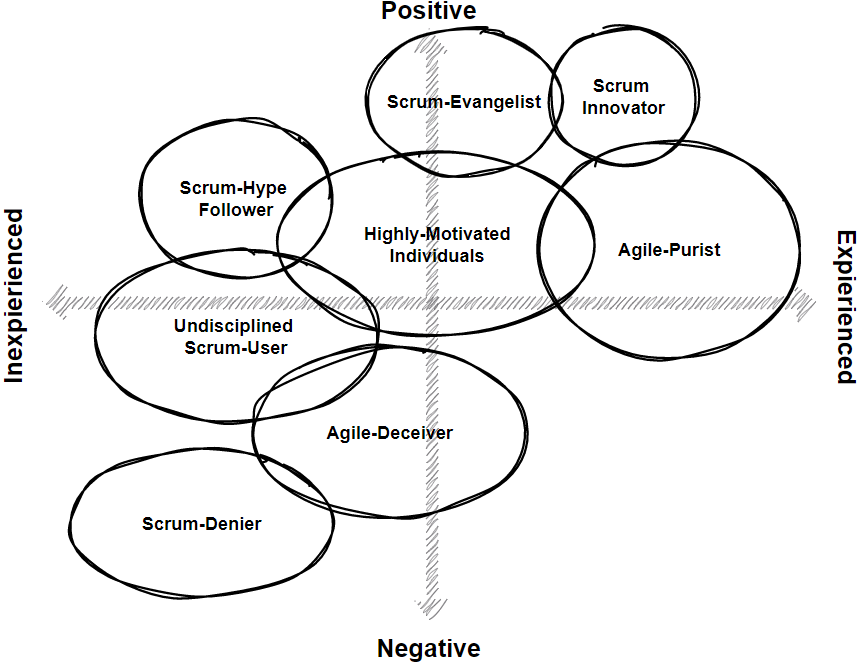
\includegraphics[width=360pt]{./assets/images/opinions-on-scrum.png}}
        \caption{Characters from literature and their views on Scrum}\label{fig:characters-of-agile}
    \end{center}
\end{figure}

% provides a comprehensive understanding
% associated dimension and attribute
\takeaways{
    This section provided a review of previous studies on the theory-practice gap of Scrum, its historical evolution, and its implementation in organizations. Scrum's success has led to the development of various \glspl{framework} based on its \gls{methodology}, including the \ac{safe} and \ac{less}. The latest revisions of the Scrum Guide have emphasized the importance of small teams, clarified the role of the Scrum Master and artifacts, and simplified the language to make it more accessible to a wider audience beyond IT. However, deviations in the roles of Scrum can lead to misunderstandings and frustration, with only one-fourth of organizations following the \glspl{guideline} set forth in the Scrum Guide. In implementing Scrum, reducing command and control structures and changing culture and leadership is important. The ideal situation is where everyone leads themselves, with a flat team model and middle management serving as servant leaders. The client's involvement is crucial for success. Investing in training is recommended to align staff in a common \gls{mindset} and improve product selling. Scaling Scrum's \gls{methodology} in larger organizations requires careful planning and execution to ensure its effectiveness. However, scaling Scrum requires mature individuals, teams, and culture. There are various views and approaches to Scrum, and each has its own impact on the success of the \gls{methodology}. In conclusion, the key takeaway is that the historical evolution of Scrum reflects the growing popularity and continuous efforts to improve its practices and outcomes and that organizations must continuously inspect and adapt their processes to make Scrum effective.
}

\section{Synthesis of findings from previous studies}\label{sec:SynthesisPreviousStudies}
The purpose of this section is to synthesize the findings from previous studies on the theory-practice gap of Scrum. By analyzing the existing body of knowledge, this section aims to provide an overview of common themes and patterns across previous studies. Furthermore, the section will discuss the contributions made by these studies to our overall understanding of the theory-practice gap of Scrum. Finally, the section will identify the gaps in the existing body of knowledge that need further investigation. By doing so, this section will provide a comprehensive overview of the current state of knowledge on the theory-practice gap of Scrum, which will serve as a foundation for future research in this area.

% Summary of common themes and patterns across previous studies
\subsection*{Summary of common themes and patterns}\label{subsec:SummaryOfCommonThemes}
In this analysis, prevalent themes from the existing body of knowledge on the \gls{transformation} or \gls{adaptation} of Scrum in organizations are examined. It has been observed that common misconceptions regarding the roles, \gls{methodology}, and effectiveness of Scrum can result in problematic \glspl{adaptation} due to factors such as lack of training, abstract nature of the \gls{framework}, or inadequate \gls{commitment} to full organizational \gls{transformation}. These issues are rooted in the organizational culture and maturity, as well as the organization's overall goals.

To address these misconceptions, one common solution is to add command and control structures and phase-based sprints rather than goal-oriented sprints. 

Another approach is to reintroduce traditional roles, which often undermines the benefits of flat hierarchical teamwork. Misperceptions about the effectiveness of Scrum at scale are frequently addressed by incorporating control structures and compromising on the \gls{agile} mindset, instead of promoting self-management and iterative product design among \gls{self-managing} teams.

Collaborating with \glspl{client} (when the organization utilizing Scrum is not the \gls{client}) can also pose challenges for organizations early in their \gls{transition}. Attempts to incorporate risk management into the Scrum \gls{methodology} may result in a hit-or-miss development process in phases, rather than involving the domain expert (the \gls{client}) in every increment. It is recommended to train the \gls{client} with internal experts to formulate their ideas for the development teams they engage, rather than predetermining fixed budgets and deadlines.

Failed \glspl{adaptation} or \glspl{transformation} of organizations often stem from a lack of research into which \gls{framework} would best fit the organization's needs. A partial \gls{transformation} that only involves the development team and ignores the rest of the organization may lead to a revert back to traditional \glspl{methodology}. To mitigate this, organizations can seek guidance from external qualified experts who can train management in becoming servant leaders and gradually building trust among former departments.

% Discussion of the contributions of the section to the overall understanding of the theory-practice gap in Scrum 
\subsection*{Discussion of the contribution to the overall undestanding of the theory-practice gap}\label{subsec:DiscussionTheoryPracticeGap}
In this section, the contribution of this thesis to the overall understanding of the theory-practice gap is discussed. The review of existing literature related to the success of Scrum and other \ac{asd} \glspl{framework}, as well as the theory-practice gap, highlights the importance of considering the individual needs of each organization in the implementation process.

The literature suggests that for organizations to realize the full benefits of Scrum, extensive research into their employees' needs, employee training and building trust, ongoing inspection of the Scrum \gls{adoption} status, and collaboration with the \gls{customer} are crucial. However, despite these insights, organizations still face challenges in the \gls{transition} to Scrum, indicating gaps in the current body of knowledge.

\quotethis{If you adopt only one agile practice, let it be retrospectives. Everything else will follow.}{\citeNP{WoodyZuill2014Iya}}

These gaps include the absence of a one-size-fits-all \gls{framework}, a lack of time for researching the organization's needs, limited \gls{commitment} from top management to enforce change, inadequate training in \gls{methodology} and communication, and a need for improvement in the hiring process of external experts.

\newpage

To address these gaps in the body of knowledge, further research is needed to answer the following questions: Why do organizations treat \glspl{framework} as ready-made solutions? Why is there a tendency to rush the process? Why is change management not receiving sufficient support from top management? Why is training in \gls{methodology} and communication not given enough importance? Why are external experts necessary? How can the hiring process of external experts be optimized?

The literature highlights several partial suggestions to address the identified gaps in the implementation of Scrum. According to \citeA[p.~2169]{vanWaardenburg2013Wam}, \ac{asd} serves as a means to identify organizational problems, rather than solving them. 

\citeA[p.~iv]{Rubin2012ESA} emphasizes the importance of listening to the employees' concerns and promoting organizational culture alignment through collaborative decision-making~\cite[p.~234]{Rubin2012ESA}. \citeA[p.~26]{Naseem2009Saa} recommend allocating budget for training early in the \gls{transformation} process. \citeA[pp.~9--13]{Wang2018Taa} advocate for experimenting with the \gls{framework} to gain valuable insights.

Additionally, \citeA[pp.~5--10]{Rubin2012ESA} recommends the use of the Cynefin Framework to determine the suitability of Scrum for an organization. \citeA[p.~101]{Theobald2019Csa} present a model, the Subway Map of Scaling Frameworks, which can assist in comparing different \glspl{framework}.

It is crucial to acknowledge that the failure of a \gls{framework} to meet the needs of an organization does not necessarily indicate a flawed \gls{framework}. However, \citeA[pp.~123--124]{Suryaatmaja2019Tmf} highlight that \glspl{framework} often lack guidance on how to adopt them, which would prove valuable to organizations exploring its use.

\takeaways{
    In this section, the theory-practice gap of Scrum is analyzed. The gap is attributed to common misconceptions about the roles, \gls{methodology}, and effectiveness of Scrum, which stem from the organizational culture, maturity, and goals. The literature stresses the importance of extensive research into employee needs, employee training, building trust, ongoing inspection of the Scrum \gls{adoption} status, and collaboration with the \gls{customer} for organizations to realize the benefits of Scrum. However, organizations still encounter challenges during the \gls{transition} to Scrum, highlighting gaps in the current knowledge base, including the absence of a one-size-fits-all framework, limited \gls{commitment} from top management, inadequate training in \gls{methodology} and communication, and a need for improvement in the hiring process of external experts. Further research is required to address these gaps, including understanding why organizations view \glspl{framework} as ready-made solutions, why change management lacks support, why training in \gls{methodology} and communication is undervalued, and why external experts are necessary. Partial solutions to these gaps include considering the individual needs of each organization, listening to employee concerns, investing in training, experimenting with the framework, and utilizing \glspl{framework} such as Cynefin and Subway Map of Scaling Frameworks.
}
%----------------------------------------------------------------------------------------
%	Debug options
%----------------------------------------------------------------------------------------
% chktex-file 2
% chktex-file 8
% chktex-file 11
% chktex-file 13
% chktex-file 18
% chktex-file 36
% chktex-file 39
% chktex-file 44
%----------------------------------------------------------------------------------------
\chapter{Method}\label{cha:Method}
% # Why does this section matter?
% # How does it reflect on investigating the gap in Scrum
% # Transition to the next section
This chapter outlines the processes and techniques used to collect and analyze data. It provides an overview of the research design, data collection \glspl{method}, and data analysis techniques employed in the study. The purpose of this chapter is to establish the credibility and reliability of the research by demonstrating the validity and rigor of the \glspl{method} used to collect and analyze data. In addition, it sets the foundation for the rest of the study and provides a clear understanding of the research process.

\section{Research design}\label{sec:Researchdesign}
% Why for what reason
In Chapter~\ref{cha:LiteratureReview}, various reasons and potential solutions for the theory-practice gap were identified. To ensure the validity of this research and bridge the gap between theoretical knowledge and practical application, the evaluation of practitioners is essential. The objective of the data collection is to gain a deeper understanding of the Scrum \gls{framework} in practice, to examine and expand upon the problems identified in literature. The outcome should provide insights into why individuals use Scrum, the challenges they face, and potential solutions and best practices for practitioners.

% Who is targeted
The target demographic for this study consists of individuals who have worked with, are currently working with, or have experience in the integration of the Scrum \gls{framework}. This interview aims to gather data from Software Developers, \gls{agile} coaches, managers, \ac{ux} designers, and any other individuals involved in developing or managing a product with Scrum.

\section{Data collection method}\label{sec:Datacollectionmethod}
% General: Number of questions, how many quantitative, how many open
The questionnaire employed in this study consisted of 42 questions, which were divided into 7 sections. 7 of the questions were multiple choice, 11 were range questions, and 24 were open-ended questions. The interview began with general questions regarding the participants' current role and organization. It then progressed to inquiries about specific \glspl{method} and \glspl{framework} used, followed by open-ended questions regarding the reasons for \gls{adoption}, challenges encountered, and the solutions they tried. The penultimate section comprised an evaluation part where the participants were presented with a list of reasons, challenges, and solutions, and asked to indicate the extent to which they had encountered them. The interview concluded with an open-ended question for participants to add any information that was not covered in the previous sections.

% Tool used
The interview tool, Google Forms, was selected due to its capability to provide accessible mobile support and convenient data analysis. Additionally, it also facilitated the ease of distribution and participation in the survey. The interview was conducted in German as the majority of the target organizations and communities were German-speaking.

% View questionnaire in the appendix
A complete listing of the questions posed during the interview can be located in the appendix under the label "\nameref{app:Questionnaire}." The corresponding responses provided by the interview participants can be found in the appendix under the heading "\nameref{app:QuestionnaireResults}".

% From when to when
The data for the Interview was collected from January 7th to January 25th, 2023. 

% How were interview participants selected
Invitations were distributed to various sources including educational institutions, alumni networks, professional communities on social media platforms (Xing, LinkedIn, and Facebook), as well as events hosted on gathering platforms (Meetup), and companies that market themselves as Scrum experts. 

% How many were there in the end
A total of 12 individuals participated in the study, with their anonymity making it difficult to accurately determine the number of organizations represented, however, it is estimated that a minimum of 8 organizations were represented. Among the participants, 25\% were associated with organizations involved in the development of websites or web-based products, while 16\% provided training and consulting services.

\section{Participants}\label{sec:Participants}
% Reference to the annex for the list of interview partners (6/12 were named)
A comprehensive list of the Interview participants wishing to be referenced in this thesis and suitable for reference purposes can be located in the appendix labeled "\nameref{app:ListOfParticipants}". To protect the privacy of six out of the twelve participants, who wished to stay anonymous, their email addresses were removed from the data and appendix.

\section{Data analysis methods}\label{sec:Dataanalysismethods}
The collected data was systematically processed to facilitate analysis. After the data collection was deemed sufficient and the deadline was reached, the raw data collected through Google Forms was formatted and transferred into a \href{https://github.com/mai-space/mai-joel_maximilian-bachelor_thesis/raw/main/assets/data/data-formated-for-analysis.xlsx}{spreadsheet}\footnote{The \href{https://github.com/mai-space/mai-joel_maximilian-bachelor_thesis/raw/main/assets/data/data-formated-for-analysis.xlsx}{spreadsheet} can be downloaded by clicking the word \href{https://github.com/mai-space/mai-joel_maximilian-bachelor_thesis/raw/main/assets/data/data-formated-for-analysis.xlsx}{spreadsheet} or by scanning the QR Code provided in the appendix under the chapter "\nameref{app:QRCode}"} linked with the questionnaire. The data was then divided into its original types, multiple choice, open-ended, and range questions, to enable easier processing and analysis.

The open-ended questions were especially challenging to analyze due to the wide range of values they provided. Thus, the answers were simplified into concise statements to facilitate comparison. The range questions, together with simple open questions, offered insights into the relationships between the demographic and organizational characteristics of the participants.

The multiple-choice questions were easily visualized after they were formatted, allowing for the drawing of meaningful conclusions. The results, in their final form, provide a valuable body of knowledge for comparison with the existing literature and may lead to interesting findings.
%----------------------------------------------------------------------------------------
%	Debug options
%----------------------------------------------------------------------------------------
% chktex-file 2
% chktex-file 8
% chktex-file 11
% chktex-file 13
% chktex-file 18
% chktex-file 36
% chktex-file 39
% chktex-file 44
%----------------------------------------------------------------------------------------
\chapter{Results and discussion}\label{cha:Discussion}
% # Why does this section matter?
% # How does it reflect on investigating the gap in Scrum
% # Transition to the next section
% Synthesize the findings in literature and method
% Derrive findings from that
Through the synthesis of findings from the literature review and the \gls{methodology} used in this thesis, this chapter aims to provide a comprehensive understanding of the challenges faced by Scrum practitioners.

The chapter is structured into four main sections, each of which focuses on a different aspect of the investigation. The first section, \fancyref{sec:Findingsfromdatacollection}, presents the results of the empirical data collected through the \gls{methodology} used in this thesis.

The second section, \fancyref{sec:Comparisonofresultswithpreviousstudies}, compares the findings of this investigation with those of previous studies on the topic. This comparison provides a nuanced understanding of the challenges faced by Scrum practitioners and how they have evolved over time.

The third section, \fancyref{sec:Interpretationoftheresults}, provides an in-depth interpretation of the findings from the data collection and comparison with previous studies. This section highlights the key challenges faced by Scrum practitioners and how they impact the implementation of the \gls{methodology}.

Finally, the fourth section, \fancyref{sec:Implicationsoftheresults}, discusses the practical implications of the findings for Scrum practitioners and organizations. This section provides recommendations in form of \glspl{guideline} for how organizations can overcome the challenges faced in implementing Scrum and how future research can address the gaps identified in this investigation.

In summary, this chapter provides a comprehensive understanding of the gap between the theory and practice of Scrum by synthesizing the findings from both the literature and \gls{methodology}.

\section{Results from data collection}\label{sec:Findingsfromdatacollection}
This section is a crucial aspect of this chapter as it presents the results of the empirical data collected through the \gls{methodology} used in this thesis. This section highlights the findings of the primary research conducted to explore the gap between the theory and practice of Scrum. The results presented in this section provide a deep insight into the challenges faced by Scrum practitioners and organizations in implementing the \gls{methodology} effectively.

This section will lay the foundation for the subsequent sections, where the findings will be compared with previous studies, interpreted, and discussed in terms of their implications. In this section, the findings are presented in a clear and concise manner, providing a comprehensive overview of the results of the research.

The composition of the businesses represented among the interviewees in this study was analyzed. 25\% of the businesses were classified as Microenterprises and 25\% as Small Businesses. Medium enterprises accounted for only 8.33\% while Large enterprises represented 41.67\%. 

In terms of \gls{agile} \glspl{methodology}, Scrum was utilized by 58.33\% of the businesses, a Hybrid approach combining Scrum and Waterfall was used by 16.67\%, \ac{safe} by 16.67\% and 8.33\% employed the adapted \ac{less} \gls{methodology}. A notable observation was that 40\% of the Large enterprises in the study utilized the \ac{safe} \gls{framework}.

The results of this study provide insights into the utilization of the Scrum \gls{framework}. According to the data, approximately 48.57\% of the surveyed individuals adhere to the textbook definition of Scrum. The average duration of a Scrum Sprint was determined to be 1.57 weeks, with 41.7\% of the interviewees indicating that they employ a two-week Sprint. 

The average team experience with Scrum was found to be 3 years, while the average personal experience with the \gls{framework} was 7 years. This should be sufficient for a team to notice the problems they face and for an individual to be able to reflect on the maturity of the organization and their integration.

35\% of the teams utilizing Scrum reported having received some form of training, while 50\% of the interviewees using the \gls{framework} indicated that they have read the Scrum Guide. The most widely referenced version of the Scrum Guide was found to be the 2013 edition, with versions from 2011 and 2020 tied for second place. 

Approximately 42.86\% of the Scrum users held a certificate from a company or organization, with 100\% of the \ac{safe} users holding a certificate for either Scrum or \ac{safe}. The Scrum users believed that holding a certificate offered more expertise compared to not holding one, while \ac{safe} users believed it provided only a minimal increase in knowledge beyond the basics. Neither group believed that holding a certificate made someone an expert in their role or the \gls{framework}. 

With regards to \glspl{transformation}, 33.33\% were accompanied by \gls{agile} coaches, 25\% were accompanied by \acp{pm}, and a smaller proportion, less than 25\%, were executed solely by the team.

In terms of integration success, Scrum users rated their success at 76.79\%, while Hybrid users rated their success at 62.5\% and \ac{safe} users at 56.25\%. The individual utilizing the adapted \ac{less} \gls{framework} reported a successful integration. 

The products developed by the interviewees encompass web-based solutions for \glspl{client}, software development, and a variety of services. An analysis of the responses provided by Scrum users revealed that 28.57\% of them perceived their approach to be insufficient for their product, with variability noted across different projects. However, none of the interviewees expressed that their approach was inappropriate for their product. 

An examination of the four \glspl{framework} revealed that the average self-assessment for self-management among Hybrid users was the lowest at 60\%, with Scrum users exhibiting the second lowest average at 68.57\%. 

The average motivation for Scrum users to switch to a different \gls{framework} was found to be the lowest, at 37.14\%, in comparison to Hybrid or \ac{safe} users. The user of the adapted \ac{less} \gls{framework} demonstrated the lowest average motivation for a change, at 20\%, when compared to the average of the other three \glspl{framework}.

\begin{figure}[!ht]
	\begin{center}
        \makebox[\textwidth]{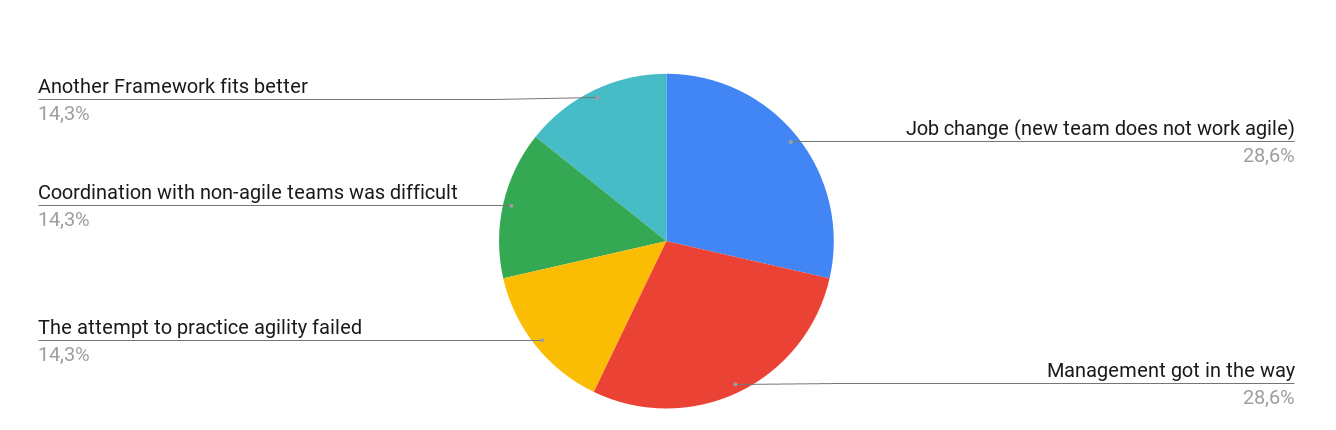
\includegraphics[width=\textwidth]{./assets/images/reasons-to-change.png}}
        \caption{Reasons to change to a different framework other than Scrum}\label{fig:reasons-to-change}
    \end{center}
\end{figure}

The Figure~\ref{fig:reasons-to-change} visualizes the most picked options for the Scrum practitioners. 

28.6\% of the respondents stated that they would move away from the Scrum \gls{framework} due to a job change or that their management got in the way of their Scrum integration. 14.3\% stated that other reasons for a change in their \gls{methodology} would be another better fitting \gls{framework}, difficult coordination with non-agile teams or that their attempt to practice agility failed

Of the 12 participants interviewed, not all provided answers to the question of which departments within their organizations utilize Scrum. However, among those who did provide answers, it was reported that 100\% of the development department employed Scrum. Additionally, among the Scrum users, 50\% of the project management department and 25\% of the \ac{ui} and \ac{ux} department utilized Scrum. 

The data shows that, among the organizations that use Scrum, 86\% on average reported using Daily Scrums, Sprint Reviews, and Backlog Refinements. On average, 71\% reported using Retrospectives and Sprint Plannings. 57\% reported using a digital Kanban board, while 43\% reported using User Stories, Story Points, and Planning Poker. The usage of alignment and control \glspl{method}, such as the Definition of Ready and Done, was reported by 14\% of the Scrum-using organizations.

Organizations of the medium size reported the highest usage of these \gls{agile} \glspl{method}, followed by small businesses, and then large organizations. Microenterprises reported the lowest usage.

The results of this study indicate that small and medium-sized organizations experience fewer difficulties in integrating Scrum compared to microenterprises and large enterprises. On average, small and medium-sized organizations reported encountering 8 out of the 38 potential issues associated with the integration process, as identified in the relevant literature. In contrast, microenterprises and large enterprises reported encountering 23.5 of the 38 potential difficulties on average. 

The most frequently reported problems with Scrum as a \gls{framework} among the interviewees were: (1) resistance from management to relinquish control; (2) lack of experienced personnel; (3) a large number of stakeholders; and (4) limitations on the influence of \gls{agile} coaches and Scrum masters imposed by management (reported by 29\% of interviewees on average). Other Problems are represented in Figure~\ref{fig:problems-with-scrum}.

\begin{figure}[!ht]
	\begin{center}
        \makebox[\textwidth]{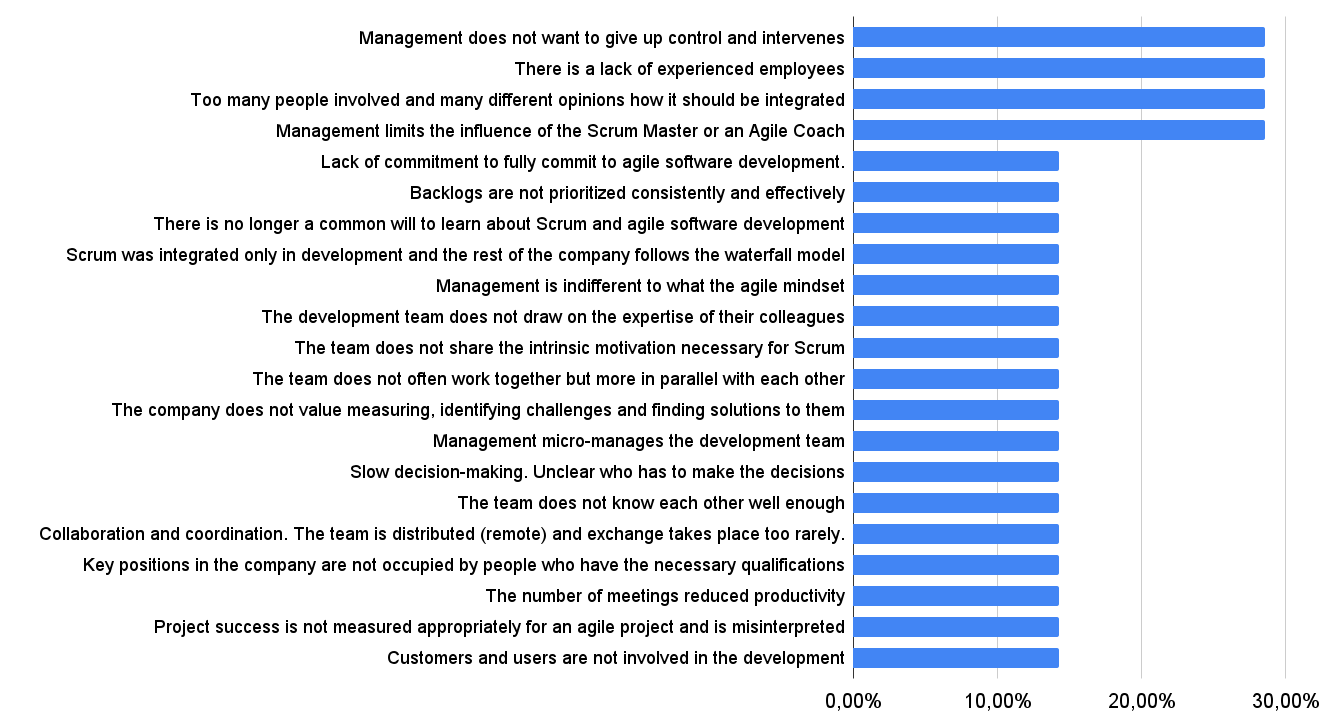
\includegraphics[width=\textwidth]{./assets/images/problems-with-scrum.png}}
        \caption{Reported average frequency of problems with Scrum}\label{fig:problems-with-scrum}
    \end{center}
\end{figure}

The results of this study suggest that a common approach to address difficulties encountered during the integration of \ac{asd} and the Scrum \gls{framework} is through training. Approximately 57\% of the respondents reported that training in \ac{asd} and the Scrum \gls{framework} was the most tried solution. Additionally, 43\% reported that training in feedback and communication culture was also a solution attempted, which indicates further challenges with the \gls{adoption} of new cultural beliefs within the organization. Yet, 57\% may still be too low as the respondents still reported problems with their \gls{adoption} related to lack of alignment and common beliefs.

To address the difficulties encountered, 43\% of the respondents reported trying the Scrum \gls{framework} for a certain period of time and following the Scrum Guide closely. Another 43\% reported solutions such as transparent communication of strategic and operational goals by management and utilizing Daily Scrums for efficient planning and coordination, which seems to be the logical solution to problems in this direction.

However, 29\% of the respondents reported not using demos and product increments for \gls{customer} and \gls{client} testing. Another 29\% reported that they had management support in writing for their \gls{adoption}, but only 14\% reported that middle management had learned new tasks and relinquished control.

Approximately 71\% of the interviewees using Scrum as their \gls{framework} reported not incorporating Concept Sprints with \glspl{client} for upfront design and planning, furthermore reducing the benefits of collaboratively working together with \glspl{client} on-site. This reinforces the widely held view that Scrum lacks design and planning upfront. Additionally, none of the interviewees utilizing Scrum as their \gls{framework} reported utilizing dedicated Enhancement Sprints.

Among the \glspl{framework}, including Scrum, the Hybrid of Scrum and Waterfall, and \ac{safe}, the Interviewees utilizing Scrum reported on average the most benefits (6 out of 8). Small businesses and medium-sized enterprises reported the most benefits from their \gls{adoption} of the Scrum \gls{framework}, and this trend was also observed with the \gls{adoption} of any new \gls{framework} different from Scrum. 

Approximately 71.43\% of the Scrum practitioners reported improved predictability, transparency, and visibility, aligning with the key goals of the Scrum \gls{framework}. Additionally, 57.14\% reported reduced risks and enhanced teamwork, which may indicate that \ac{asd} aligns with human collaboration and thinking processes. 42.86\% reported enhancements in effectiveness, productivity, team morale, product quality, and \gls{client} satisfaction, which are common outcomes associated with \ac{asd}, as validated by the findings of this study. Furthermore, 42.86\% reported the utilization of faster feedback from real users, which may have led to improved product quality and \gls{client} satisfaction.

\section{Comparison of results with previous studies}\label{sec:Comparisonofresultswithpreviousstudies}
This section provides a nuanced understanding of the challenges faced by Scrum practitioners by comparing the findings of this investigation with those of previous studies on the topic. The comparison of results with previous studies provides a more complete picture of the gap between the theory and practice of Scrum and enables a deeper understanding of the current state of the field.

The comparison in this section not only highlights the similarities and differences between the results of this investigation and previous studies, but also sheds light on the unique contributions of this study. The results of the comparison provide a solid basis for the interpretation of the findings and help to establish the significance of this study in the larger context of research on the topic.

\subsection*{Deviations and Challenges}\label{subsec:DeviationsandChallenges}
This study expands upon the existing literature on the implementation of the Scrum \gls{methodology} by showcasing deviations from the prescribed Sprint \gls{methodology} detailed in the Scrum Guide. The study findings reveal an average Sprint length of 1.57 weeks and 41.7\% of respondents utilizing 2-week Sprints. However, the study departs from previous research, as described in section~\fancyref{subsubsec:UnderstandingSprints}, by not finding the use of dedicated Enhancement Sprints~\cite[p.~2]{Sutherland2005Fos}. The current study offers valuable insight by suggesting that organizations considering the \gls{adoption} of Scrum should experiment with the \gls{framework} before making any alterations~\cite[pp.~9--13]{Wang2018Taa}, as also described in section~\fancyref{subsec:DiscussionTheoryPracticeGap}.

\subsection*{Limited Departmental Participation}\label{subsec:LimitedDepartmentalParticipation}
The study presents empirical evidence that supports prior research by disclosing that the majority of participants report that the development department is the primary user of Scrum, with limited involvement from other departments~\cite[p.~233]{Rubin2012ESA}, as previously discussed in section~\fancyref{subsubsec:TransformingTheMethodology}.

Moreover, the study extends the current body of literature by indicating a correlation between the success of Scrum implementation, the number of challenges faced, organizational culture, and the degree of participation from departments outside of development such as management~\cite[p.~125]{Moreira2013AtA}, which was also mentioned in section~\fancyref{subsubsec:TransformingManagement}.

\subsection*{Low Engagement}\label{subsec:LowEngagement}
This study provides further support for the prevalent belief that there is limited engagement with the Scrum \gls{methodology} among the participants and their teams. This aligns with previous research highlighting the need for comprehensive training and shared understanding of the \gls{methodology}~\cite[p.~72]{Maximini2018ISi}, found in section~\fancyref{subsubsec:BudgetingTrainging}. The study also adds to the existing literature by indicating that variations in the \glspl{guideline} prescribed within the Scrum Guide may result in different interpretations within teams. Additionally, the data highlights the significance of external expertise, as none of the participants considered certification as a marker of expertise in their role or the \gls{framework}, which partially confirms the hypothesis from section~\fancyref{subsubsec:DeviationOfRoles}, that Scrum Masters lack expertise and therefore \gls{agile} coaches with experience get hired.

\subsection*{Challenges in Client Collaboration}\label{subsec:ChallengesinClientCollaboration}
The study provides empirical evidence that supports previous research conclusions regarding the limited participation of \glspl{client} in organizations implementing Scrum, leading to difficulties in collaboration. Section~\fancyref{subsubsec:SellingScrum} stated the criticality of the involvement of the \gls{client} in the development process~\cite[p.~5]{Coyle2009Acs}.

\subsection*{Adoption and Success Across Organizational Size and Maturity}\label{subsec:AdoptionSuccessOrganizationalSize}
This study confirms prior research findings that larger enterprises tend to adopt scaling \glspl{framework}~\cite[p.~50]{Moreira2013AtA} and extends these findings by suggesting that simple \glspl{framework} such as Scrum may be easier to implement compared to complex systems like \ac{safe}, confirming former research~\cite[p.~119]{Gall1986SHs} presented by section~\fancyref{subsubsec:ChoosingAFramework}. The study also presents evidence of a positive correlation between the use of \gls{agile} \glspl{method}, lower problems, and greater benefits among small to medium-sized organizations. However, it is essential to note that further investigation is necessary to thoroughly evaluate the cultural differences that may exist between different organization sizes.

\subsection*{Adoption and Evolution of the Scrum Framework}\label{subsec:AdoptionEvolutionScrum}
The present study concurs with prior research in that the majority of Scrum practitioners are still predominantly from software development departments. However, this study also observes a growing trend of Scrum \gls{adoption} in non-software departments~\cite[Revision 2010--2013]{Schwaber2020SGR} as described in section~\fancyref{subsec:historyOfScrum}.

This study supports the prior findings, described in section~\fancyref{subsubsec:EmbracingSelfManagement}, that hybrid approaches to Scrum tend to yield low self-assessment scores in terms of self-management~\cite[p.~24]{Koning2019AT}, although it departs from existing literature by revealing that Scrum itself exhibits similarly low levels of self-management. The study further confirms the significance of management in the successful \gls{adoption} of a new \gls{framework}~(\citeNP[p.~125]{Moreira2013AtA};~\citeNP[pp.~37--38]{Boehm2005Mct}), in accordance with previous studies found in section~\fancyref{subsubsec:TransformingManagement}. The study contributes to the existing body of knowledge by uncovering a limited utilization of alignment \glspl{method} as prescribed by the Scrum guide, despite their potential to enhance collaboration and effectiveness.

\section{Interpretation of the results}\label{sec:Interpretationoftheresults}
This section provides an in-depth understanding of the gap between the theory and practice of Scrum. Through an analysis of the findings from the data collection and comparison with previous studies, this section highlights the key challenges faced by Scrum practitioners and how they impact the implementation of the \gls{methodology}.

This section goes beyond simply presenting the results and provides an in-depth examination of the findings to understand the underlying causes and effects of the challenges faced by Scrum practitioners. In this section, the results are not only presented but also analyzed and interpreted to provide a deeper understanding of the key challenges faced by Scrum practitioners.

The interpretation of the results provides a basis for the discussion of the practical implications of the findings, which is presented in the subsequent section.

The findings of this study are consistent with prior research that highlights the need for extensive training and shared understanding in the implementation of Scrum. This study also supports the notion that smaller and medium-sized organizations may be more flexible in adapting to new \glspl{methodology}. However, further investigation is needed to fully evaluate any cultural differences between organizations of different sizes. The low levels of self-organization within organizations utilizing Scrum suggest challenges in integrating the culture, while reduced \gls{client} involvement in testing processes indicate issues with client-collaboration. This study also confirms the critical role of management in the \gls{adoption} of new \glspl{framework} and the impact of uneven distribution and \gls{commitment} to the culture on participation from other departments.

This study extends the existing body of knowledge by examining the impact of different versions of the Scrum Guide on the integration of Scrum. The results suggest that variations in the Scrum Guide may lead to different understandings, making it a factor to consider. The study also found that organizations heavily rely on external experts, implying a need for more internal investment in training and building expertise. Deviations from the Sprint \gls{methodology} may reflect conscious change management decisions or difficulties in transitioning to Scrum. Further research is needed to fully assess the impact of Sprint length. The study highlights the value of organizations conducting their own research and avoiding unthinking adherence to \glspl{framework}.

\newpage

The findings of this study diverge from previous research that found simpler \glspl{framework} to be easier to implement with fewer difficulties compared to complex \glspl{framework}. The discrepancy between the results may be due to differences in \gls{methodology} or sample population. Although the latest revision of the Scrum Guide has aimed to simplify the \gls{framework}, the study suggests that more clarification is needed regarding alignment \glspl{method} and strategies for successful \gls{adaptation}. Further research is necessary to reconcile conflicting results and determine the root causes of the discrepancy.

The results of this study challenge prior research that found close collaboration to be a significant benefit of Scrum. This study found that the level of testing and collaboration with \glspl{client} was lower than expected, indicating that Scrum and \ac{asd} are often utilized as process enhancements rather than full cultural shifts. Further research is needed to reconcile this contradiction and establish a more accurate understanding of the topic.

\section{Implications of the results on the adoption of Scrum}\label{sec:Implicationsoftheresults}
This section discusses the practical implications of the findings for Scrum practitioners and organizations. The results of the investigation into the gap between the theory and practice of Scrum provide valuable insights into the challenges faced in implementing the \gls{methodology} effectively. This section takes those results a step further by providing recommendations for how organizations can overcome the challenges and providing a roadmap for organizations looking to implement Scrum effectively.

In addition to the practical implications, this section also provides insights into future research opportunities that can help address the gaps identified in this investigation. The discussion in this section provides direction for future research and contributes to the ongoing conversation about the theory and practice of Scrum.

% key findings, implications, recommendations
% Some of the common challenges faced by organizations include management interference with the self-management of the Scrum team, insufficient guidance from Scrum Masters, a lack of psychological safety in the organizational culture, limited involvement of \glspl{client} and \glspl{customer}, differing perceptions and understandings of the Scrum \gls{framework}, inadequate employee involvement in the \gls{adoption} process, and a lack of understanding of how to effectively utilize \glspl{framework} and provide adequate training to employees.
The findings of this study emphasize the importance of organizations conducting their own research and adopting \glspl{methodology} that are most suitable for their specific needs and circumstances. This may include factors such as the product being developed, \gls{client} characteristics, and organizational size.

The study highlights the importance of involving all departments in the \gls{transition} to a new \gls{methodology} to ensure a shared understanding and enhanced alignment. Relying solely on external experts may not provide the necessary internal investment in training and building expertise.

The results of this study also highlight the crucial role of management in the successful \gls{adoption} of new \glspl{methodology}, and the implications of uneven distribution and \gls{commitment} to the culture for participation from other departments. This may require training and time for managers to effectively \gls{transition} into leaders.

Overall, these findings provide valuable insights for practicing organizations and contribute to a more comprehensive understanding of the factors that influence the successful integration of \gls{agile} \glspl{methodology}. 

\newpage

From these insights and the knowledge from the literature, \glspl{guideline} can be derived that help the practitioners of Scrum. The \glspl{guideline} are as follows: 

\begin{enumerate}
    \item Due to the continuous evolution of the Scrum \gls{framework} and \ac{asd}, organizations that want to adopt the \gls{methodology} and \gls{ideology} have to do their own research on the topic.
    \item In addition, organizations have to require the needs of their teams and involve them in the decision-making processes and listen to the critics.
    \item Training the employees is crucial, in order to hold common knowledge among the team about the \glspl{method} and processes in use.
    \item Organizations must implement inspect-and-adapt cycles not only for the products they develop but their processes too. They will provide the necessary agility for the teams to thrive and the organization to evolve.
    \item Top management has to support the \gls{transformation} from the start in order to provide the psychological safety needed for the new roles and \glspl{mindset} to mature.
    \item If the \gls{adoption} stagnates, the hiring of external experts such as \gls{agile} coaches can be beneficial.
    \item Scaling Scrum's \glspl{method} to multiple or larger teams is secondary to the establishment of culture since the teams will struggle more with the \gls{adoption} of a new \gls{methodology} that is complex and fully fletched out with no room for \gls{adaptation} than with guiding \glspl{mindset} and simplified \glspl{method}.
\end{enumerate}

% future research
The following represent areas of inquiry that future research may consider in order to expand upon the understanding of the implementation and integration of Scrum:

\begin{enumerate}
    \item Further investigation of the effects of cultural differences on the successful \gls{adoption} of Scrum in organizations of different sizes.
    \item Further analysis of the impact of Sprint length on the outcomes and benefits of Scrum implementation.
    \item Comparison of the benefits and limitations of fully-fleshed out \glspl{framework} versus those that are simplified or adapted.
    \item Examination of the influence of revisions of the Scrum Guide on the \gls{transition} process for organizations.
    \item Exploring the reasons for the difficulties organizations encounter in collaboration with \glspl{client}.
    \item Investigation of the root causes of the challenges organizations face in collaboration with \glspl{client} during the \gls{adoption} of Scrum.
\end{enumerate}
%----------------------------------------------------------------------------------------
%	Debug options
%----------------------------------------------------------------------------------------
% chktex-file 2
% chktex-file 8
% chktex-file 11
% chktex-file 13
% chktex-file 18
% chktex-file 36
% chktex-file 39
% chktex-file 44
%----------------------------------------------------------------------------------------
\chapter{Conclusion}\label{cha:Conclusion}
% # Why does this section matter?
% # How does it reflect on investigating the gap in Scrum
% # Transition to the next section
% Conclude what have been learned, refer to the research question(s), refer to literature, compare findings
This chapter brings the investigation into the gap between the theory and practice of Scrum to a close. It presents a summary of the findings from the literature review and data collection and provides an overview of the practical implications of the results. The conclusion provides a final synthesis of the research question and the key findings and draws a clear connection between the investigation and its implications for both practice and future research.

% What is the theory-practice gap of Scrum?
% Provide common knowledge about Scrum and the theory-practice gap
% what are its characteristics?
The first research question guiding this thesis is "What is the theory-practice gap of Scrum?". The theory-practice gap of Scrum can be characterized by splitting it up into three dimensions "language", "\gls{methodology}" and "evolution". While the "language" dimension refers to deviations, lack of verbalization and misunderstandings about the \gls{methodology} of Scrum and its effectiveness, the dimension "\gls{methodology}" has attributes like how existing roles and \glspl{method} or processes can be transformed, how the \gls{adoption} of Scrum can be strategically planned and how the \gls{framework} could be scaled up to larger teams and organizations. The third dimension "evolution" visualizes the attributes in which Scrum has been changed up and improved, for example through scaling \glspl{framework} or moving away from prepared \glspl{framework} and embracing the \ac{agile-manifesto} and its \gls{ideology}.  

% what are the perceptions of Scrum practitioners regarding the challenges faced?
% Identify the challenges faced by Scrum practitioners
% Explore the perceptions of Scrum practitioners
% Investigate the impact of the theory-practice gap on organizations and teams
The second research question of this thesis is "What are the perceptions of Scrum practitioners regarding the challenges faced?". This literature review and study have confirmed that the theory-practice gap of Scrum had many implications for organizations and teams. They often correlated with the lack of support, training, involvement and \gls{commitment}. Among the reported issues were the lack of involvement of the employees and the lack of involvement of the \gls{client} in the testing processes. This has led to a reduced alignment of the teams and missed opportunities for greater \gls{client} satisfaction. Another issue reported in the literature and this study is the lack of support through upper management and the lack of \gls{commitment} of other departments than development to the \gls{adoption} of the \gls{framework}, which has led to frustration for the \glspl{developer} and reduced benefits of Scrum.

% what were their solutions tried and what guidelines can be derived from them?
% Provide insights for organizations and practitioners to improve their implementation of Scrum
The third research question providing a goal for this thesis is "what were the solutions tried and what guidelines can be derived from them?". The various solutions tried most often lead to the same conclusions that can be drawn from them. To observe the successful \gls{adoption} of a \gls{framework}, an organization has to listen carefully to the requirements their employees have and commit to the change. Further implications for practitioners are explained in the next section.

\newpage

\section{Guidelines for the adoption of Scrum}\label{sec:Implicationsforpractice}
% # Why does this section matter?
% # How does it reflect on investigating the gap in Scrum
% # Transition to the next section
% Recommend a set of methods or behavior guidelines on how to solve the individual gap
This section provides a summary of the practical implications of the findings for Scrum practitioners and organizations. It provides a clear overview of the recommendations for overcoming the challenges faced in implementing Scrum and offers practical guidance for organizations looking to implement the \gls{methodology} effectively. The implications for practice are based on a thorough analysis of the results and provide actionable recommendations for organizations looking to adopt Scrum.

The evolution of the Scrum \gls{framework} has been the subject of ongoing research, with contributions from the original authors and practitioners in the field. \Gls{adoption} of the Scrum \gls{framework} in organizations has been found to be influenced by a variety of factors, including organizational size, maturity, culture, and knowledge of the \gls{framework}. 

To address these challenges, organizations can prioritize the needs of their employees, consider the input of critics, research available \glspl{methodology} and \glspl{framework}, invest in employee training, and involve employees in the decision-making process. By adopting an inspect-and-adapt cycle, organizations can continuously refine their custom \gls{methodology} and ensure its ongoing value. However, resolving issues of collaboration with \glspl{client} and cultural differences within organizations may require letting go of resistant employees and educating \glspl{client} about the benefits of \ac{asd}. The support of top management is crucial for the success of the \gls{adoption} and \gls{transformation} process, and Scrum Masters and Agile Coaches can provide valuable guidance in this regard.

Scaling Scrum to accommodate larger teams or multiple products can be accomplished through the use of scaling \glspl{framework}. However, it is recommended to first establish a strong foundation in \Gls{agile} \glspl{principle}, potentially through the use of Scrum, before exploring scaling \glspl{framework} and adapting them to fit the specific needs of the organization. Keeping the \gls{methodology} simple and avoiding complexity is crucial in ensuring the effectiveness of the scaling process.

\section{Limitations of the study}\label{sec:Limitationsofthestudy}
% # Why does this section matter?
% # How does it reflect on investigating the gap in Scrum
% # Transition to the next section
% The Interviewee Count is far below what I had anticipated. But the answers given by the Interviewees are interesting enough that I am convinced that the analysis will provide sufficient Inside into this matter, but I am also convinced that a much broader Study of this topic will probably be able to go even more in-depth.
This section highlights the limitations of the investigation into the gap between the theory and practice of Scrum. It provides an overview of the limitations of the \gls{methodology} used in this thesis and the limitations of the results. The conclusion of the limitations of the study provides important context for interpreting the results and understanding the limitations of the investigation.

Despite the ongoing efforts of practitioners and authors to enhance the understanding and address emerging issues, the literature on this subject is constantly evolving and subject to change. As the field of Software Development advances quickly, it is possible that new research and insights may emerge that further shed light on the Scrum theory-practice gap.

The study was designed to gather data through the administration of questionnaires, however, the response rate was lower than anticipated. Despite this, the results obtained were sufficient to identify key areas of concern for organizations and provide support for previous literature on the subject. 

It is recommended that future studies with higher participation and a more diverse sample population be conducted to provide a more comprehensive understanding of the Scrum theory-practice gap.

The results of this study serve as a useful starting point for further research and exploration into the complexities of the Scrum theory-practice gap. While the results provide interesting observations and indicate potential areas for further research, caution must be exercised in interpreting the results and making conclusive statements. A larger sample size or other \glspl{methodology} may be necessary to fully validate the findings of this study.

\section{Future research on the theory-practice gap of Scrum}\label{sec:Implicationsforfutureresearch}
% # Why does this section matter?
% # How does it reflect on investigating the gap in Scrum
% # Transition to the next section
% What were the limitations of the research
% What was done well, what can be done in the future
This section provides areas in which future research can build upon the findings of this investigation and provides direction for future investigations into the gap between the theory and practice of Scrum. The implications for future research are based on a thorough analysis of the results and provide a roadmap for advancing the field of study.

The results of previous studies and the present study raise several questions regarding the \gls{adoption} and implementation of the Scrum \gls{framework}. The following topics warrant further investigation:

\begin{description}[style=nextline]
    \item[The use of external experts in organizations]
    Understanding why organizations rely so heavily on external experts and why their use is so prevalent could provide valuable insights into how organizations can better optimize the hiring process and manage the role of these experts.
    \item[The perceived simplicity of frameworks]
    It is important to understand why organizations treat \glspl{framework} as ready-made solutions and why there is a tendency to rush the process.
    \item[Change management]
    Further research is needed to investigate why change management is not receiving sufficient support from top management and how organizations can address this issue.
    \item[Training in methodology and communication]
    The importance of training in \gls{methodology} and communication needs to be better understood, and the impacts and requirements for training in feedback and communication culture need to be explored.
    \item[Cultural differences and organization size]
    Investigating the impacts of cultural differences inside organizations of different sizes could provide valuable insights into how organizations can better address these differences.
    \item[Sprint length]
    The impact of sprint length on the implementation and success of the Scrum \gls{framework} needs to be studied in greater detail.
    \item[Advantages and disadvantages of fully-featured frameworks]
    A more in-depth analysis of the benefits and disadvantages of fully-featured \glspl{framework} could provide valuable insights into how organizations can optimize their \gls{adoption} and implementation of Scrum.
    \item[Impacts of revisions to the Scrum Guide]
    Understanding the impact of revisions to the Scrum Guide on transitioning organizations is crucial in order to resolve different understandings of Scrum and refine the \gls{framework}.
    \item[Client collaboration]
    Further research is needed to understand why organizations struggle with \gls{client} collaboration and what the reasons for this struggle are. This could provide valuable insights into how organizations can better address these issues and improve collaboration with \glspl{client}.
\end{description}
    
\par\noindent\rule{\textwidth}{0.4pt}

Although Software Development and the \glspl{framework} guiding its processes are always changing, it is worth it to investigate the causes of issues and derived solutions on a regular basis. The body of knowledge around the practices of Software Development and working together collaboratively will evolve in the future and with the increasing usage of artificial intelligence and new opportunities in communication, future researchers may find some of the problems and solutions presented by this thesis to be outdated. As for now, this study has investigated currently faced issues and presented \glspl{guideline} for organizations, on how they can adopt the Scrum \gls{framework} without facing the issues of the theory-practice gap.

\newpage

%	Appendix
\pagenumbering{Roman}
\setcounter{page}{6}
%----------------------------------------------------------------------------------------
%	Debug options
%----------------------------------------------------------------------------------------
% chktex-file 2
% chktex-file 8
% chktex-file 11
% chktex-file 13
% chktex-file 18
% chktex-file 36
% chktex-file 39
% chktex-file 44
%----------------------------------------------------------------------------------------
\chapter{Appendix}
%----------------------------------------------------------------------------------------
%	List of Acronyms
%----------------------------------------------------------------------------------------
\section{Acronyms}\label{sec:acronyms}
% # 
% # Usage:
% # \ac{kürzel} = Erstes Mal Langform mit (Kürzel) dann nur noch Kürzel mit Link zum Acronym
% # \acl{kürzel} = gibt nur die Langform der Abkürzung aus mit Link zum Akronym
% # \acp{kürzel} || \aclp{kürzel} = Selbes wie oben nur mit Plural version
% # 
%----------------------------------------------------------------------------------------
%	Debug options
%----------------------------------------------------------------------------------------
% chktex-file 36
% chktex-file 39
% chktex-file 18
% chktex-file 8
% chktex-file 11
%----------------------------------------------------------------------------------------
%	Usage options
%----------------------------------------------------------------------------------------
% \acf{po} (Product Owner (PO))
% \ac{po} (product owner)(po)
% \Ac{po} (Product Owner)(Po)
% \acp{po} (Product Owners)(POs)

\begin{acronym}[HCD]
    \acro{ux}[UX]{User-Expierience}
    \acro{ui}[UI]{User-Interface}
    \acro{po}[PO]{Product Owner}
    \acroplural{po}[POs]{Product Owners}
    \acro{pm}[PM]{project manager}
    \acroplural{pm}[PMs]{project managers}
    \acro{safe}[SAFe]{Scaled Agile Framework}
    \acro{less}[LeSS]{Large-Scale Scrum}
    \acro{agile-manifesto}[Agile Manifesto]{Manifesto for Agile Software Development}
    \acro{asd}[ASD]{Agile Software Development}
    \acro{dod}[DoD]{Defintion of Done}
\end{acronym}

%----------------------------------------------------------------------------------------
%	List of Glossaries
%----------------------------------------------------------------------------------------
\newpage
\printnoidxglossaries%

%----------------------------------------------------------------------------------------
%	List of Interviewees
%----------------------------------------------------------------------------------------
\newpage
\section{List of Participants}\label{app:ListOfParticipants}

\textbf{Normen Möller}\newline
{Freelancer}\newline
\icontext{Xing}{14}{\href{https://www.xing.com/profile/Normen_Moeller/cv}{Normen$\_$Moeller}}{black}

\textbf{Sonja Zuckerstätter BA MSc}\newline
{Content Managerin}\newline
\textit{content garden technologies GmbH}\newline
\icontext{Linkedin}{14}{\href{https://www.linkedin.com/in/sonja-zuckerstaetter}{sonja-zuckerstaetter}}{black}

\textbf{Norman Günther}\newline
{IT Project Manager | Agile Coach}\newline
\textit{BZ.medien Digital}\newline
\icontext{Xing}{14}{\href{https://www.xing.com/profile/Norman_Guenther4/cv}{Norman$\_$Guenther4}}{black}

\textbf{Michael Spiller}\newline
{Senior Agile Coach}\newline
\textit{metafinanz Informationssysteme GmbH}\newline
\icontext{Linkedin}{14}{\href{https://linkedin.com/in/michaelspiller}{michaelspiller}}{black}

\textbf{Mario Hirschfeld}\newline
{Agile Coach} \newline
\textit{L.N. Schaffrath DigitalMedien GmbH}

\textbf{Jean-Pierre Berchez}\newline
{Gesellschafter} \newline
\textit{HLSC GmbH}\newline
\icontext{Linkedin}{14}{\href{https://www.linkedin.com/in/jpberchez/}{jpberchez}}{black}

\newpage
\section{Link to the spreadsheet used for analysis}\label{app:QRCode}
To download the spreadsheet through your Browser, click this link right \textcolor{Violet}{\href{https://github.com/Inf166/mai-joel_maximilian-bachelor_thesis/raw/main/assets/data/data-formated-for-analysis.xlsx}{here}}.

Alternatively, you can scan this QR Code with your phone camera:
\begin{figure}[!ht]
    \makebox[128pt]{
\includegraphics[width=128pt]{./assets/images/qr-code-to-the-spreadsheet-github.png}}
\end{figure}

\section{How to cite this thesis}
\subsection*{BibTex}
\begin{lstlisting}[label={lst:HowToCite}]
@MastersThesis{MaiGrotenKullack2023IttpoS,
author           = {Mai, Joel Maximilian and Groten, Raphaela and Kullack, Sven},
title            = {{Investigating} the theory-practice gap of {Scrum}},
year             = {2023},
month            = {02},
type             = {Bachelor's Thesis},
journal          = {Technische Hochschule Koeln},
keywords         = {scrum, agile software development, framework, methodology, theory-practice gap}
}
\end{lstlisting}

\begin{description}
    \item[MLA] Mai, Joel Maximilian, et al. Investigating the Theory-Practice Gap of Scrum. 02 2023.
    \item[APA] Mai, J. M., Groten, R., \& Kullack, S. (02 2023). Investigating the theory-practice gap of Scrum.
    \item[AMA] Mai JM, Groten R, Kullack S. Investigating the Theory-Practice Gap of Scrum. 02 2023.
    \item[IEEE] J. M. Mai, R. Groten, and S. Kullack, 'Investigating the theory-practice gap of Scrum', 02 2023.
    \item[Harvard] Mai, J. M., Groten, R. and Kullack, S. (02 2023) Investigating the theory-practice gap of Scrum.
    \item[Chicago] Mai, Joel Maximilian, Raphaela Groten, and Sven Kullack. 'Investigating the Theory-Practice Gap of Scrum', 02 2023.
\end{description}
%----------------------------------------------------------------------------------------
%	List of References
%----------------------------------------------------------------------------------------
\bibliographystyle{apacite}
\renewcommand{\refname}{List of References}
\bibliography{bibliography/biblio.bib}

%----------------------------------------------------------------------------------------
%	List of Figures
%----------------------------------------------------------------------------------------
\newpage
\listoffigures
	
%----------------------------------------------------------------------------------------
%	List of Tables
%----------------------------------------------------------------------------------------
%\newpage
%\addcontentsline{toc}{chapter}{List of Tables}
%\listoftables

%\newpage

%----------------------------------------------------------------------------------------
%	Questionnaire
%----------------------------------------------------------------------------------------
%----------------------------------------------------------------------------------------
%	Debug options
%----------------------------------------------------------------------------------------
% chktex-file 1
% chktex-file 2
% chktex-file 8
% chktex-file 11
% chktex-file 13
% chktex-file 18
% chktex-file 26
% chktex-file 36
% chktex-file 39
% chktex-file 44
%----------------------------------------------------------------------------------------
\newpage
\section{Questionnaire}\label{app:Questionnaire}
\einzelantworticon = Single-choice question; \checkboxantworticon = Multiple-choice question

\section*{Über mich}
Ich heiße Joel Maximilian Mai und bin 24 Jahre alt. Zur Zeit studiere ich Medieninformatik an der Technischen Hochschule Köln. Für meine Bachelorarbeit und aus eigenem Interesse beschäftige ich mich viel mit agilen Frameworks, Methoden und ins besondere Scrum. Da ich selbst Webentwickler bin, interessiere ich mich sehr für den besten Weg Software zu entwickeln. 

\section*{Was ist der Grund für die Umfrage?}
Das Thema meiner Bachelorarbeit ist "Investigating the Theory-Practice Gap of Scrum". In der Theorie klingt Scrum sinnvoll und klar. Jedoch werden Frameworks häufig in der Theorie erweitert und für die Anwendung in der Praxis angepasst. Während meiner Literatur Recherche konnte ich viele Gründe und Lösungsansätze für die Herausforderungen aber auch für den Gap identifizieren. Jedoch, um nicht selbst einen Gap zwischen Literatur und Praxis zu erzeugen, benötige ich die Evaluierung meiner Ergebnisse durch eine Umfrage.

\section*{Welchem Zweck soll die Umfrage dienen?}
Mit Ihrer Unterstützung möchte ich mehr über den Gebrauch des Scrum Frameworks in der Praxis erfahren. Ich möchte erfahren, was gut läuft und die von mir in der Literatur identifizierten Probleme hinterfragen und ergänzen. Ich bin interessiert an den Gründen, warum Sie Scrum anwenden und an den Ursachen möglicher Herausforderungen. 

\section*{Danke für Ihre Teilnahme}
Ich danke Ihnen herzlich für die Teilnahme. Dieses Thema interessiert mich ganz besonders. Die Ergebnisse dieser Studie und der Arbeit werden hoffentlich anderen begeisterten Menschen bei ihrem Weg helfen.

\textit{Diese Umfrage dauert etwa 15 Minuten.}

\section*{Über Sie}
In diesem Abschnitt erfasse ich die zuvor genannten Rahmendaten um später in der Analyse Zusammenhänge zwischen der Position und Erfahrung und den beschriebenen Herausforderungen herzustellen.

\section*{Wie lautet ihre aktuelle Berufsbezeichnung?}
\kurzantwort

\section*{Wie lange arbeiten Sie schon in dem Bereich? (in Jahren)}
\kurzantwort

\section*{Hatten Sie bereits Erfahrung in einer anderen Rolle/Position, wenn ja, in welchen?}
\kurzantwort

\section*{Unternehmen und Team}
In diesem Abschnitt erfasse ich Rahmendaten über die Unternehmen um später Zusammenhänge zwischen der Größe, der Anzahl der Herausforderungen aber auch welche Herausforderungen besonders häufig auftreten herzustellen.

\section*{Wie groß ist das Unternehmen in dem Sie eingestellt sind aktuell?}
\einzelantwort{Kleinstunternehmen (weniger als 10 Personen)}
\einzelantwort{Kleinunternehmen (10-49 Personen)}
\einzelantwort{mittleres Unternehmen (50-249 Personen)}
\einzelantwort{Großunternehmen (mehr als 250 Personen)}

\section*{Welches Produkt bietet ihr Unternehmen an? (eigene Software, Webseiten für Kunden, ...)}
\kurzantwort

\section*{Wie groß ist Ihr aktuelles Team?}
\kurzantwort

\section*{An wie vielen Projekten arbeitet Ihr Team durchschnittlich gleichzeitig?}
\kurzantwort

\section*{Agile Frameworks, Agile Methoden}
Mir ist bewusst, dass viele Unternehmen nicht ausschließlich Scrum verwenden, daher erfasse ich in diesem Abschnitt die Abweichung von dem eigentlichen Scrum Guide.

\section*{Welche der folgenden agilen Methoden nutzen Sie?}
\einzelantwort{Scrum}
\einzelantwort{Scrumban}
\einzelantwort{Scrum-eXtreme Programming Hybrid}
\einzelantwort{Kanban}
\einzelantwort{Iterative}
\einzelantwort{Lean Thingking}
\einzelantwort{Weitere ...}

\section*{Für welches der folgenden Frameworks hat sich Ihr Unternehmen entschieden?}
\einzelantwort{Scrum (Nach Jeff Sutherland und Ken Schwaber)}
\einzelantwort{Disciplined Agile}
\einzelantwort{Scrums of Scrums (Jeff Sutherland)}
\einzelantwort{Nexus}
\einzelantwort{Scrum@Scale}
\einzelantwort{Enterprise Scrum}
\einzelantwort{Scaled Agile Framework (SAFe)}
\einzelantwort{Large Scale Scrum (LeSS)}
\einzelantwort{Agile Portfolio Management}
\einzelantwort{Weitere ...}

\section*{Wie sehr hält sich Ihr Unternehmen dabei an das Framework?}
\skalarvonbis{1}{10}{gar nicht}{strikt nach Lehrbuch}

\section*{An welchen Stellen weicht Ihr Unternehmen von der Theorie ab?}
\langantwort

\section*{Für wie gravierend halten Sie den Einfluss dieser Abweichung auf den Erfolg der Scrum Integration?}
\skalarvonbis{1}{5}{unbedeutend}{gravierend}

\section*{Hatten Sie bereits Erfahrung mit einem der anderen genannten Frameworks?}
\checkboxantwort{Scrum (Nach Jeff Sutherland und Ken Schwaber)}
\checkboxantwort{Disciplined Agile}
\checkboxantwort{Scrums of Scrums (Jeff Sutherland)}
\checkboxantwort{Nexus}
\checkboxantwort{Scrum@Scale}
\checkboxantwort{Enterprise Scrum}
\checkboxantwort{Scaled Agile Framework (SAFe)}
\checkboxantwort{Large Scale Scrum (LeSS)}
\checkboxantwort{Agile Portfolio Management}
\checkboxantwort{Weitere ...}

\section*{Welche der folgenden Methoden nutzt Ihr Unternehmen aktiv?}
\checkboxantwort{Daily Stand-Up}
\checkboxantwort{Retrospektiven}
\checkboxantwort{Sprint/Iterations Review}
\checkboxantwort{Sprint/Iterations Planning}
\checkboxantwort{Backlog Refinement}
\checkboxantwort{Digital Kanban Board}
\checkboxantwort{User Stories und oder Epics}
\checkboxantwort{Story Points}
\checkboxantwort{Planning Poker / Schätzungen}
\checkboxantwort{Häufige Releases}
\checkboxantwort{Work in Progress Limits}
\checkboxantwort{Physikalisches Kanbanboard}
\checkboxantwort{Weitere ...}

\section*{Wie lange dauert ein Sprint bei Ihnen in Wochen? (0 für keine Sprints)}
\einzelantwort{0}
\einzelantwort{1}
\einzelantwort{2}
\einzelantwort{3}
\einzelantwort{4}
\einzelantwort{Weitere ...}

\section*{Bestandsaufnahme: Scrum}
Um jetzt aber doch bessere Schlüsse ziehen zu können um den Gap von Scrum zu definieren, erfasse ich im folgenden Abschnitt explizite Daten zu der Erfahrung mit Scrum und das Erlernen des Frameworks.

\section*{Wie lange arbeitet Ihr Team bereits mit Scrum?}
\einzelantwort{Aktuell noch in der Testphase}
\einzelantwort{Kürzer als ein Jahr}
\einzelantwort{1-2 Jahre}
\einzelantwort{3-5 Jahre}
\einzelantwort{5 Jahre und mehr}

\section*{Wie lange arbeiten Sie schon mit Scrum? (in Jahren)}
\kurzantwort

\section*{Haben Sie schon einmal den Scrum Guide gelesen?}
\einzelantwort{Ja}
\einzelantwort{Teilweise}
\einzelantwort{Nein}

\section*{Wenn Sie sich bereits mit einer Veröffentlichung des Scrum Guides beschäftigt haben, mit welcher? (Jahr genügt)}
\kurzantwort

\section*{Welche Abteilungen nutzen Scrum in Ihrem Unternehmen? (Projektmanagement, HR, UX, UI, Konzeption, Entwicklung...)}
\langantwort

\section*{Wie viele Teammitglieder haben eine aktive Auseinandersetzung mit der Theorie von Scrum abgeschlossen und somit ein ausgeprägtes Verständnis?}
\kurzantwort

\section*{Welche Quelle halten Sie für Wertvoll um sich das Scrum Framework anzueignen?}
\langantwort

\section*{Wenn Sie ein Zertifakt für Scrum oder eine der Rollen besitzen, von welcher Quelle?}
\kurzantwort

\section*{Wie würden Sie die Expertise bewerten, die ein solches Zertifikat vermittelt?}
\skalarvonbis{1}{5}{Basiswissen}{Experte in dem Framework/Rolle}

\section*{Was waren Gründe oder Ursachen für ihr Unternehmen, das Framework Scrum zu wählen?}
\langantwort

\section*{Zu dem Gap in der Praxis}
Dieser Abschnitt ist wahrscheinlich der wichtigste von allen. Er bietet Ihnen die Möglichkeit den Erfolg der Integration von Scrum einzuschätzen und die wichtigsten Herausforderungen als auch Lösungsansätze sowie Tipps zu äußern. 

\section*{Wie würden Sie den Erfolg der Integration von Scrum in Ihrem Unternehmen bewerten?}
\skalarvonbis{1}{8}{Gescheitert}{Voller Erfolg}

\section*{Was sind die Herausforderungen der Integration von Scrum gewesen?}
\langantwort

\section*{Was waren Lösungsansätze mit denen Ihr Unternehmen versucht hat die Herausforderungen zu lösen?}
\langantwort

\section*{Welche Herausforderungen blieben bis heute bestehen?}
\langantwort

\section*{Welche Ratschläge würden Sie anderen Unternehmen, Teams oder Kollegen mitgeben um die Integration und Adaption von Scrum zu erleichtern?}
\langantwort

\section*{Halten Sie Scrum für ungeeignet für Ihren Anwendungszweck?}
\einzelantwort{ungeeignet}
\einzelantwort{projektabhängig}
\einzelantwort{geeignet}

\section*{Welche Rollen oder Methoden wurden von dem Alten mit in den neuen Prozess übernommen und warum? (z.B. bei Wasserfall -> Scrum, könnte das Projektmanager sein oder Anforderungsmanagement)}
\langantwort

\section*{Wer leitete Ihre Transformation/den Übergang zu Scrums Methoden? (Rolle/Position)}
\langantwort

\section*{Wie schätzen Sie die Selbstorganisation und das Selbstmanagement Ihres Teams ein?}
\skalarvonbis{1}{5}{von außen kontrolliert}{selbst organisiert}

\section*{Wie hoch ist Ihre Motivation Scrum durch ein anderes Framework zu ersetzen?}
\skalarvonbis{1}{5}{niedrig}{hoch}

\section*{Welches Framework empfehlen Sie alternativ?}
\kurzantwort

\section*{Was wären die Gründe für die Anwendung eines anderen Frameworks?}
\checkboxantwort{Jobwechsel (Neues Team arbeitet nicht agil)}
\checkboxantwort{Jobwechsel (Kein Programmierer mehr)}
\checkboxantwort{Management war im Weg}
\checkboxantwort{Aktueller Prozess ist ähnlich aber nicht agil}
\checkboxantwort{Der Versuch Agilität zu praktizieren schlug fehl}
\checkboxantwort{Die Koordination mit nicht agilen Teams war schwierig}
\checkboxantwort{Die Projekte litten unter schlechtem Design}
\checkboxantwort{Weitere ...}

\section*{Bekannte Herausforderungen und deren Lösungsansätze}
Dieser Teil ist fast so bedeutsam wie der vorherige. Hier möchte ich Ihnen zeigen welche Erkenntnisse ich durch die Literatur erlangen konnte. Ich brauch jedoch Ihre Hilfe dabei mir zu bestätigen welche der Gründe, Herausforderungen und Lösungsansätze tatsächlich in Ihrer Praxis stattfanden. Gerne dürfen Sie mir im Anschluss an die Umfrage Fragen zu den einzelnen Punkten stellen.

\section*{Welche der folgenden Gründe waren es, die zur Integration von Scrum in Ihrem Unternehmen gesorgt haben?}
\checkboxantwort{Vorhersehbarkeit, Transparenz und Sichtbarkeit}
\checkboxantwort{Frühe Risiko-Reduktion}
\checkboxantwort{Schnelleres Deployment an den Kunden oder Testumgebung}
\checkboxantwort{Schnelleres Return on Investment}
\checkboxantwort{Schnelleres Feedback von echten Nutzern}
\checkboxantwort{Kundenzufriedenheit ist verbessert}
\checkboxantwort{Reibungslosere Teamarbeit}
\checkboxantwort{Software Qualitätsverbesserung}
\checkboxantwort{Effektivitätsverbesserung}
\checkboxantwort{Mehr automatisiertes Testing}
\checkboxantwort{Produktivitätsverbesserung}
\checkboxantwort{Bessere Produkte für Kunden und Nutzer entwickeln}
\checkboxantwort{Verbessern von Reaktion auf sich verändernde Anforderungen und Prioritäten}
\checkboxantwort{Verbesserung von Einigkeit von Unternehmen und Entwicklern}
\checkboxantwort{Verbesserte Moral im Team}
\checkboxantwort{Anforderungsänderungen fallen leichter}
\checkboxantwort{Management entschied sich dafür}

\section*{Welche der folgenden Herausforderungen hatte Ihr Unternehmen bei der Integration von Scrum?}
\checkboxantwort{Es wurde nicht geprüft ob agile Software Entwicklung sinnvoll für das Unternehmen ist}
\checkboxantwort{Langsame Entscheidungsfindung. Zunächst ist nicht nur unklar wer die Entscheidungen zu treffen hat, aber auch die Informationsweitergabe erfolgt träge oder passiv.}
\checkboxantwort{Fehlendes Commitment sich ganz und gar der agilen Software Entwicklung zu verschreiben.}
\checkboxantwort{Es gibt keinen gemeinsamen Willen mehr über Scrum und agiler Software Entwicklung zu lernen}
\checkboxantwort{Die Integration von der agilen Kultur endete mit der Bekanntmachung von Scrum im Unternehmen}
\checkboxantwort{Fehlendes agiles Mindset und Kultur. Die Meinungen über die Sinnhaftigkeit eines agilen Mindsets wird nicht von allen geteilt}
\checkboxantwort{Zu viele Personen involviert. Viele verschiedene Meinungen über was Scrum ist und wie es integriert werden sollte}
\checkboxantwort{Scrum wurde von einen auf den anderen Tag etabliert und hat viel Schaden angerichtet}
\checkboxantwort{Es fehlenen erfahrene Mitarbeiter}
\checkboxantwort{Das Unternehmen legt keinen Wert darauf zu messen, Herausforderungen zu identifizieren und Lösungen für diese zu finden}
\checkboxantwort{Scrum wurde nur in der Entwicklung Integriert und der Rest des Unternehmens folgt dem Wasserfall Modell}
\checkboxantwort{Der Geschäftsführung ist es gleichgültig was das agile Mindset ist und sieht keinen Grund selbst Veränderungen im Unternehmen anzuordnen}
\checkboxantwort{Das Management will keine Kontrolle über die Teams abgeben und greift in die Arbeit ein}
\checkboxantwort{Das Management limitiert den Einfluss des Scrum Masters oder eines Agile Coaches}
\checkboxantwort{Das Management entschied agil zu werden ohne Abstimmung im Team}
\checkboxantwort{Das Management mikro-managet das Entwickler-Team}
\checkboxantwort{Der Scrum Master hat nicht die Qualifikation um bei der Integration von Scrum im Unternehmen zu helfen}
\checkboxantwort{Kollaboration und Koordination. Das Team ist verteilt (remote) und Austausch findet zu selten statt.}
\checkboxantwort{Das Entwickler Team greift nicht auf die Expertise ihrer Kollegen zurück}
\checkboxantwort{Das Team teilt nicht die für Scrum notwendige intrinsische Motivation}
\checkboxantwort{Das Team hat nicht die Erlaubnis entscheidungen selbst zu treffen}
\checkboxantwort{Das Team hat nicht das selbe Ziel wie das Unternehmen}
\checkboxantwort{Das Team kennt sich nicht gut genug}
\checkboxantwort{Das Team arbeitet nicht häufig zusammen sondern mehr parallel zueinander}
\checkboxantwort{Es wird nicht regelmäßig für die Inkremente des Produkts Kunden-/Nutzerfeedback gesammelt}
\checkboxantwort{Es wird kein Budget freigegeben für Fortbildungen zur Integration von agiler Software Entwicklung}
\checkboxantwort{Die Räumlichkeiten und Zusammenarbeit hat sich nicht verändert um Scrum-basiertes Arbeiten zu ermöglichen}
\checkboxantwort{Informationen über den Projektstatus werden nicht regelmäßig kommuniziert}
\checkboxantwort{Die Backlogs wird nicht konsequent und effektiv priorisiert}
\checkboxantwort{Schlüsselpositionen im Unternehmen sind nicht von Personen besetzt die die notwendige Qualifikation besitzen}
\checkboxantwort{Alte Positionen wurden nicht durch die neuen Rollen und Weiterbildungen ersetzt}
\checkboxantwort{Die Anzahl der Meetings reduzierte die Produktivität}
\checkboxantwort{Es gab kein Upfront-Design / Konzeption und oder blieb bei einem niederen Design}
\checkboxantwort{Entwickler die später am Projekt arbeiten, sind nicht Teil des Teams welches die Planung und Konzeption vollzieht}
\checkboxantwort{Erfolg des Projekts wird nicht angemessen für ein agiles Projekt gemessen und fehlinterpretiert}
\checkboxantwort{Kunden und Nutzer werden nicht die Entwicklung mit einbezogen}
\checkboxantwort{Kunden verstehen den Sinn von Konzeption und Anforderungsermittlung}
\checkboxantwort{Der Kunde hält agile Software Entwicklung für riskanter und versteht nicht die Vorteile}

\section*{Welche der folgenden Lösungsansätze hatte auch Ihr Unternehmen versucht?}
\checkboxantwort{Scrum nach Lehrbuch für bestimmte Zeit durchführen}
\checkboxantwort{Geschäftsführung um Rückendeckung für die Integration und Durchführung bitten und schriftlich festhalten}
\checkboxantwort{Training in agile und Scrum für alle Beteiligten}
\checkboxantwort{Training in Feedback- und Kommunikations-Kulur für alle Beteiligten}
\checkboxantwort{Enhancement-Sprints für Low-Prio Backlog Items}
\checkboxantwort{Concept Sprint(s) mit Kunden vor den eigentlichen Development-Sprints}
\checkboxantwort{Team entscheidet welches Framework/Methodologie geeignet ist}
\checkboxantwort{Kunde / Produkt Owener + Business Value (Estimation) entscheiden prio}
\checkboxantwort{Inspect-Adapt Zyklus(Retrospektiven) für die Scrum Integration wird kontinuierlich fortgeführt}
\checkboxantwort{Es wird nicht länger in Abteilungen gedacht sondern in Projektteams und Rollen}
\checkboxantwort{Keine Demos, Kunden nutzen/testen das aktuelle Produkt/Release}
\checkboxantwort{Mittleres Management lernt neue Aufgaben kennen und gibt Kontrolle ab}
\checkboxantwort{Jemand mit Erfahrung und umfassendem Wissen leitet die Transformation und begleitet diese}
\checkboxantwort{Daily Stand-Ups dienen zur Koordination für den kommenden Tag und es werden Probleme beseitigt die dem bestmöglichstem Tag im Weg stehen}
\checkboxantwort{Teams werden nach dem Dreyfus-Squared Model gepaart um bestmöglichste Ergebnisse zu erzielen}
\checkboxantwort{Der aktuelle Projekt Status wird vom Teamleiter im Daily-Standup kurz am Anfang präsentiert}
\checkboxantwort{Die Geschäftsführung kommuniziert strategische und operative Ziele transparent}
\checkboxantwort{Teammitglieder die an zusammenhängenden Teilen eines Produkts arbeiten, arbeiten im engen Austausch zusammen}
\checkboxantwort{Jeder Sprint sollte ein MVP als Ergebnis haben, welches von Kunden und Nutzern getestet werden kann}
\checkboxantwort{Nicht Abteilungen sitzen beisammen, sondern Projektteams}
\checkboxantwort{Nach einem Konzept-Workshop wird ein Design-Konzept Sprint durchgeführt welcher das Konzept in erste Prototypen überführt und zur Weiterentwicklung des Produkts beiträgt}
\checkboxantwort{Im besten Fall ist ein Kunde anwesend um das Produkt unter Beobachtung zu testen, um schnell Anpassungen an den Anforderungen vornehmen zu könnnen, substitutiv kann auch Remote getestet werden}
\checkboxantwort{Die Kunden wurden über die Vorteile von Scrum und agiler Software Entwicklung zu Beginn der Vertragsverhandlungen in Kenntnis gesetzt und eventuell Beispiele genannt bekommen}

\section*{Welche Folgen von agiler Transformation treffen auf Ihr Unternehmen zu?}
\checkboxantwort{Verbesserte Vorhersehbarkeit, Transparenz und Sichtbarkeit}
\checkboxantwort{Frühe Risiko-Reduktion}
\checkboxantwort{Schnelleres Deployment an den Kunden oder Testumgebung}
\checkboxantwort{Schnelleres Return on Investment}
\checkboxantwort{Schnelleres Feedback von echten Nutzern}
\checkboxantwort{Kundenzufriedenheit ist verbessert}
\checkboxantwort{Reibungslosere Teamarbeit}
\checkboxantwort{Software Qualitätsverbesserung}
\checkboxantwort{Effektivitätsverbesserung}
\checkboxantwort{Mehr automatisiertes Testing}
\checkboxantwort{Produktivitätsverbesserung}
\checkboxantwort{Bessere Produkte für Kunden und Nutzer entwickeln}
\checkboxantwort{Verbessern von Reaktion auf sich verändernde Anforderungen und Prioritäten}
\checkboxantwort{Verbesserung von Einigkeit von Unternehmen und Entwicklern}
\checkboxantwort{Verbesserte Moral im Team}
\checkboxantwort{Anforderungsänderungen fallen leichter}

\section*{Ihre Anmerkungen}
Wenn Sie das Gefühl haben, dass Sie gerne noch mehr zu dem Thema sagen möchten haben Sie hier die 
Gelegenheit dazu...

\section*{Haben Sie noch andere Gründe für den Theorie-Praxis Gap von Scrum?}
\langantwort

\section*{Wollen Sie die Quellen für diese Umfrage sehen?}
\einzelantwort{Ja}
\einzelantwort{Nein}

\section*{Möchten Sie für Rückfragen zu Ihren Antworten Ihre Email-Adresse angeben?}
\kurzantwort

\section*{Möchten Sie in meiner Abschlussarbeit als Interviewpartner genannt werden? (Andernfalls bleiben Sie anonym)}
\einzelantwort{Ja}
\einzelantwort{Nein}

\section*{Für die Nennung geben Sie bitte folgende Daten an:}
Titel Vorname Nachname\newline
Aktuelle Position in den Unternehmen\newline
Aktuelles Unternehmen für das Sie arbeiten\newline
(optional) Einen Link zu Ihrem LinkedIn/Xing/... Profil\newline
\langantwort

\section*{Möchten Sie nach Veröffentlichung der Abschlussarbeit benachrichtigt werden um sich die Ergebnisse durchzulesen?}
\einzelantwort{Ja}
\einzelantwort{Nein}


%----------------------------------------------------------------------------------------
%	Questionnaire Results
%----------------------------------------------------------------------------------------
%----------------------------------------------------------------------------------------
%	Debug options
%----------------------------------------------------------------------------------------
% chktex-file 1
% chktex-file 2
% chktex-file 8
% chktex-file 11
% chktex-file 13
% chktex-file 18
% chktex-file 26
% chktex-file 36
% chktex-file 39
% chktex-file 44
%----------------------------------------------------------------------------------------
\newpage
\section{Questionnaire results}\label{app:QuestionnaireResults}
\responsecount = Response count; \openresponse = Open answer of an Interviewee

Some of the results were not easily printable, therefore they are appended as graphs after the questions that were able to print. For the raw data please download the spreadsheet linked in section~\fancyref{app:QRCode}.

\section*{Wie lautet ihre aktuelle Berufsbezeichnung?}
\begin{description}
    \item[2 \responsecount] Agile Coach
    \item[1 \responsecount] Scrum Trainer / Agile Coach / Geschäftsführer
    \item[1 \responsecount] QA Consultant
    \item[1 \responsecount] Projektmanager/PO und Programmierer (selbstständig)
    \item[1 \responsecount] Consultant (Projektmanagement)
    \item[1 \responsecount] IT Project Manager
    \item[1 \responsecount] Softwareentwickler
    \item[1 \responsecount] Berater
    \item[1 \responsecount] Projektmanagement
    \item[1 \responsecount] Content Manager
    \item[1 \responsecount] Referent Entgelt
\end{description}

\section*{Wie lange arbeiten Sie schon in dem Bereich? (in Jahren)}
\begin{description}
    \item[2 \responsecount] 1 Jahr
    \item[2 \responsecount] 10 Jahre
    \item[1 \responsecount] 2 Jahre
    \item[1 \responsecount] 5 Jahre
    \item[1 \responsecount] 6 Jahre
    \item[1 \responsecount] 12 Jahre
    \item[1 \responsecount] 13 Jahre
    \item[1 \responsecount] 15 Jahre
    \item[1 \responsecount] 22 Jahre
    \item[1 \responsecount] 25 Jahre
\end{description}

\section*{Hatten Sie bereits Erfahrung in einer anderen Rolle/Position, wenn ja, in welchen?}
\begin{description}
    \item[3 \responsecount] Ja
    \item[1 \responsecount] Softwareentwicklung
    \item[1 \responsecount] (Senior) Business Consultant, IT Projekt Manager, Engagement Manager, IT Transformation Manager, Versicherungskauffrau
    \item[1 \responsecount] Teamleitung, Abteilungsleitung, Anforderungs-/Qualitätsmanagement
    \item[1 \responsecount] Administration / Entwicklung
    \item[1 \responsecount] Verwicherubngskauffrau
    \item[1 \responsecount] Berater, Enterprise Architekt, Trainer
    \item[1 \responsecount] Geschäftsführer, Country Manager Germany, Vertriebsmitarbeiter, Technischer Sales Support
    \item[1 \responsecount] Scrum Master, Agile Coach
    \item[1 \responsecount] Nein
\end{description}

\section*{Wie groß ist das Unternehmen in dem Sie eingestellt sind aktuell?}
\begin{description}
    \item[5 \responsecount] Großunternehmen (mehr als 250 Personen)
    \item[3 \responsecount] Kleinstunternehmen (weniger als 10 Personen)
    \item[3 \responsecount] Kleinunternehmen (10-49 Personen)
    \item[1 \responsecount] Mittleres Unternehmen (50-249 Personen)
\end{description}

\section*{Welches Produkt bietet ihr Unternehmen an? (eigene Software, Webseiten für Kunden, ...)}
\begin{description}
    \item[1 \responsecount] ein Produkt für die Industrie
    \item[1 \responsecount] Dienstleistung
    \item[1 \responsecount] Dienstleistung zu agilen Themen
    \item[1 \responsecount] Versicherungen
    \item[1 \responsecount] Service dienstleistungen für Entwicklung bis hin zu Marketing
    \item[1 \responsecount] Training, Workshop und 1:1 für Führungskräfte
    \item[1 \responsecount] Webseiten, Apps, Intranet, individual Entwicklung
    \item[1 \responsecount] Webbasierte Lösungen für Kunden
    \item[1 \responsecount] Webseite, Digitale Produkte
    \item[1 \responsecount] Websites und maßgeschneiderte Softwatelösungen
    \item[1 \responsecount] Content Marketing, eigene Software zur Distribution
    \item[1 \responsecount] Software
\end{description}

\section*{Wie groß ist Ihr aktuelles Team?}
\begin{description}
    \item[2 \responsecount] 5
    \item[1 \responsecount] 0
    \item[1 \responsecount] 1
    \item[1 \responsecount] 2
    \item[1 \responsecount] 6
    \item[1 \responsecount] 7
    \item[1 \responsecount] 8
    \item[1 \responsecount] 13
    \item[1 \responsecount] 20
    \item[1 \responsecount] Programm größe / Aktuelles Projekt 200+. Anzahl der Leute in den Teams mit denen ich Arbeite 20 insgesamt
    \item[1 \responsecount] 32
\end{description}

\section*{An wie vielen Projekten arbeitet Ihr Team durchschnittlich gleichzeitig?}
\begin{description}
    \item[2 \responsecount] 4
    \item[2 \responsecount] 2-3
    \item[2 \responsecount] 1
    \item[1 \responsecount] Jedes Team an je einem Projekt zur gleichen Zeit
    \item[1 \responsecount] 0
    \item[1 \responsecount] 5
    \item[1 \responsecount] 6-8
    \item[1 \responsecount] 7
    \item[1 \responsecount] 12
\end{description}

\section*{Welche der folgenden agilen Methoden nutzen Sie?}
\begin{description}
    \item[2 \responsecount] Scrum
    \item[2 \responsecount] Kanban
    \item[1 \responsecount] Scrumban
    \item[1 \responsecount] SAFe
    \item[1 \responsecount] Das Beste aus allen Welten: klassisch trifft agil und Methoden, die bisher keiner kennt
    \item[1 \responsecount] Eine Mischung aus Wasserfall und Scrum.
    \item[1 \responsecount] Agiles Projetkmanagement
\end{description}

\section*{Für welches der folgenden Frameworks hat sich Ihr Unternehmen entschieden?}
\begin{description}
    \item[7 \responsecount] Scrum (Nach Jeff Sutherland und Ken Schwaber)
    \item[2 \responsecount] Scaled Agile Framework (SAFe)
    \item[1 \responsecount] Das Beste aus allen Welten: klassisch trifft agil und Methoden, die bisher keiner kennt
    \item[1 \responsecount] Angepasstes Less
    \item[1 \responsecount] Eher eine agile Herangehensweise um für den Kunden und dem Projekt die richtige Arbeitsweise zu finden.
\end{description}

\section*{An welchen Stellen weicht Ihr Unternehmen von der Theorie ab?}
\begin{itemize}
    \item[\openresponse] An denen, wo es nicht mit der Unternehmenskultur und Unternehmenswerten übereinstimmt. An denen, wo das Framework zu starre Grenzen setzt und damit eher Mehraufwand produziert als die Zusammenarbeit fördert. Ich habe über 20 Jahre Berufserfahrung, davon 10 Jahre in der IT Beratung, daher kenne ich die guten und schlechten Seiten von allen gängigen Methoden und Frameworks
    \item[\openresponse] Rollenverteilung (PO häufig nicht verfügbar oder muss anderweitig, zB durch internen Projektmanager, vertreten werden.) - Ereignisse / Meetings (Häufig nicht in Gänze durchführbar, da Kunden nicht immer bereit sind diese vollumfänglich zu bezahlen und an diesen Stellen sparen möchte) - Daily Scrum wird häufig nur wöchentlich durchgeführt
    \item[\openresponse] Wenn Kunde und/oder Projekt es nicht hergeben, wird komplett klassisch gearbeitet. Dies betrifft kleine überschaubare Projekte, wo agil eher mit Kanonen auf Spatzen schießen wäre. Vor allem wenn der Kunde keinen Mehrwert sieht, sind jegliche Diskussionen überflüssig und kosten nur unnötig Zeit.
    \item[\openresponse] Nach der Lehrbuch SCRUM Phase (3-6 Sprints pro Team) darf das Team selbstständig per Retro Anpassungen vornehmen, die auch SCRUM nach Lehrbuch verändern können. Das sind in der Regel kleine Stellschrauben.
    \item[\openresponse] Kein Business Value an Objectives, Keine Lean Business Cases, Ungenügende Einbindung der Business Owner, Kein Continuous Deployment, Keine Einbeziehung Feedback da verzögerte System Demo
    \item[\openresponse] Hauptächlich Rollenverteilung (es gibt Überschneidungen) den Rest versuchen wir nach Lehrbuch, haben aber keinen ausgebildeten Scrum Master
    \item[\openresponse] Planung und ausführung der arbeitsschritte. Aber sind alles Integrative teams und man muss auf andere Teams warten.
    \item[\openresponse] Eingebettet in einer "alten Welt". Quasi: Scrum unter Wasserfall
    \item[\openresponse] Fokus auf ein Produkt, Daily Scrum
    \item[\openresponse] Sprintdisziplin, kaum Reviews
    \item[\openresponse] Sprints
\end{itemize}

\section*{Wie lange dauert ein Sprint bei Ihnen in Wochen? (0 für keine Sprints)}
\begin{description}
    \item[5 \responsecount] 2 Wochen
    \item[3 \responsecount] 1 Woche
    \item[2 \responsecount] 3 Wochen
    \item[1 \responsecount] Keine Sprints
    \item[1 \responsecount] Unterschiedlich, zwischen 2-4 Wochen
\end{description}

\section*{Wie lange arbeitet Ihr Team bereits mit Scrum?}
\begin{description}
    \item[4 \responsecount] 3-5 Jahre
    \item[3 \responsecount] 1-2 Jahre
    \item[3 \responsecount] 5 Jahre und mehr
    \item[2 \responsecount] Kürzer als ein Jahr
\end{description}

\section*{Wie lange arbeiten Sie schon mit Scrum? (in Jahren)}
\begin{itemize}
    \item[\openresponse] 20 Jahre
    \item[\openresponse] 15 Jahre
    \item[\openresponse] 12 Jahre
    \item[\openresponse] 10 Jahre
    \item[\openresponse] 8 Jahre
    \item[\openresponse] 7 Jahre
    \item[\openresponse] 6 Jahre
    \item[\openresponse] 4 Jahre
    \item[\openresponse] 2 Jahre
    \item[\openresponse] 1-2 Jahre
    \item[\openresponse] 1 Jahre
\end{itemize}

\section*{Haben Sie schon einmal den Scrum Guide gelesen?}
\begin{description}
    \item[8 \responsecount] Ja
    \item[3 \responsecount] Nein
    \item[1 \responsecount] Teilweise
\end{description}

\section*{Wenn Sie sich bereits mit einer Veröffentlichung des Scrum Guides beschäftigt haben, mit welcher? (Jahr genügt)}
\begin{description}
    \item[2 \responsecount] 2015
    \item[1 \responsecount] 2014
    \item[1 \responsecount] 2021 habe ich den aktuellen gelesen
    \item[1 \responsecount] 2016
    \item[1 \responsecount] 1
    \item[1 \responsecount] 2012
    \item[1 \responsecount] 2011 und 2020
\end{description}

\section*{Welche Abteilungen nutzen Scrum in Ihrem Unternehmen? (Projektmanagement, HR, UX, UI, Konzeption, Entwicklung ...)}
\begin{itemize}
    \item[\openresponse] Da ich alleine bin, nutze ich agiles arbeiten für alles, sogar mit meinen Klienten im Mentoring und Coaching
    \item[\openresponse] Projektmanagement, Backend, Frontend, Konzeption, UX, UI
    \item[\openresponse] Projektmanagement, Entwicklung, Team Digitale Produkte
    \item[\openresponse] Entwicklung, die restlichen arbeiten mit Kanban
    \item[\openresponse] Content, Projektmanagement, Development
    \item[\openresponse] Softwareentwicklung für Webprojekte
    \item[\openresponse] IT, UX, UI, teilweise Business
    \item[\openresponse] Entwicklung Projektmanagement
    \item[\openresponse] Eine Person, da selbständig.
    \item[\openresponse] Alle
    \item[\openresponse] 50\%
\end{itemize}

\section*{Wie viele Teammitglieder haben eine aktive Auseinandersetzung mit der Theorie von Scrum abgeschlossen und somit ein ausgeprägtes Verständnis?}
\begin{description}
    \item[3 \responsecount] eine Person
    \item[2 \responsecount] 5 Personen
    \item[1 \responsecount] 3 Personen
    \item[1 \responsecount] 13 Personen
    \item[1 \responsecount] 50\% des Programms wurden geschult
    \item[1 \responsecount] alle
\end{description}

\section*{Welche Quelle halten Sie für Wertvoll um sich das Scrum Framework anzueignen?}
\begin{itemize}
    \item[\openresponse] Man sollte sich generell informieren und dann für sich die sinnvollen Aspekte heraussuchen und versuchen diese pragmatisch in seiner Arbeitsweise zu implementieren. Wer denkt Scrum ist wie eine Bibel und versucht dies überall so zu implementieren, wird in der Regel scheitern oder sehr viele Diskussionen führen und dadurch mehr Zeit verbrennen als notwendig.
    \item[\openresponse] Original für die Zertifizierung und Erfahrungsberichte für die Realität
    \item[\openresponse] Scrum Agiles Projektmanagement erfolgreich einsetzen dpunkt.verlag
    \item[\openresponse] Scrum Guide, diverse Yout Tube Videos, Lego for Scrum, das Web
    \item[\openresponse] Hauptsählih Den Scrum-Guide, weitere Literatur und Erklärungen
    \item[\openresponse] Scrum Guide, Praxis und Literatur zu den Detailthemen ...
    \item[\openresponse] Scrum Guide, Scrum.org und Scrum Inc Trainings, Bücher
    \item[\openresponse] Workshop durch Experten
    \item[\openresponse] Trainings
    \item[\openresponse] Schulung
\end{itemize}

\section*{Wenn Sie ein Zertifakt für Scrum oder eine der Rollen besitzen, von welcher Quelle?}
\begin{description}
    \item[3 \responsecount] Scrum Inc.
    \item[2 \responsecount] Scrum.org
    \item[1 \responsecount] Scrum Alliance
    \item[1 \responsecount] Scaled Agile Inc.
    \item[1 \responsecount] CSPO
    \item[1 \responsecount] vmedu
\end{description}

\section*{Was waren Gründe oder Ursachen für ihr Unternehmen, das Framework Scrum zu wählen?}
\begin{itemize}
    \item[\openresponse] Bei größeren Projekten helfen die kleinen Iterationen sehr ein Projekt zu bewerten und neu zu justieren. Dem Kunden sind zu Beginn viele Dinge oft nicht klar. Anstatt am Ende ein "fertigen" Projekt zu haben, wo alles ein wenig anders ist als vorgestellt, kann man so ein deutlich besseres Produkt vorfinden, wo alle konstant aktiv mit dran gearbeitet haben. Kosten sind ebenfalls deutlich überschaubarer.
    \item[\openresponse] Klar war, dass klassisches PM nicht zielführend für komplexe Projekte ist und je größer das Projekt wird desto komplexer wurden diese auch. Offensichtlich war, dass es Alternativen geben muss und da sind wir über Scrum / Agile gestolpert.
    \item[\openresponse] Um eine erprobte Vorgehensweise nachzuahmen. Vorteile sind außerdem die regelmäßigen Planungen, kombiniert mit Zielorientierem arbeiten. Relativ großer standard in der Softwareentwicklung
    \item[\openresponse] Schnelle Anpassung, schnelles Feedback. Außerdem war es wahrscheinlich einfach hip und trendy scrum zu benutzen
    \item[\openresponse] Optimierung der bestehenden Prozesse, flexibler auf chaotische Projektumfeld reagieren
    \item[\openresponse] Schnellere Umsetzung und stärkere Kundenzentrierung
    \item[\openresponse] unseren Kunden zu helfen komplexe Themen zu lösen
    \item[\openresponse] Durch eigene Erfahrung jahrelang erprobt
    \item[\openresponse] Mehr Struktur bei mehr Agilität
    \item[\openresponse] Abkehr Wasserfall
    \item[\openresponse] gute frage
\end{itemize}

\section*{Was sind die Herausforderungen der Integration von Scrum gewesen?}
\begin{itemize}
    \item[\openresponse] Um SCRUM nicht nur als Framework sondern tatsächlich gelebt zu integrieren, bedarf es an einigen Voraussetzungen, um damit erfolgreich zu arbeiten. Meine Erfahrungen aus der Praxis: Management gibt vor, dass jetzt agil gearbeitet wird und wollen gleichzeitig kontrollieren -> agil trifft auf klassisch weder die Organisation noch die Menschen sind bereit dafür, agil zu arbeiten Die größte Herausforderung ist: einen Wandel der Unternehmenskultur und -werte auf allen Ebenen einschließlich Management, Vorstände, Geschäftsführer zu vollziehen Denn nur wenn die Menschen bereit sind und fähig sind, einem für sie neuen und unbekannten Umfeld zu arbeiten, dann kann die Integration von SCRUM durchaus zum Erfolg führen.
    \item[\openresponse] Mindset, Menschen ändern ihre Philosophie und Einstellung zur Arbeit nicht von heute auf Morgen. Sowohl die Scrum Teams als auch die Kunden haben damit Probleme gehabt. Das ist heute schon deutlich weiter. Dennoch geht es immer wieder darum "müssen" in "wollen" zu transformieren. Das Wissen über die Methode ist lächerlich einfach. Daher geht es ausschließlich um den festen Willen Agilität zu implementieren und die Geduld den Tanker langsam zu drehen.
    \item[\openresponse] Durch einige Faktoren ist die Integration von scrum nach Lehrbuch häufig nicht 1:1 möglich. Die Herausforderung besteht darin scrum als Tool zu sehen und so zu integrieren, dass es ins jeweilige Unternehmen passt.
    \item[\openresponse] Story Point vergeben und planen. Anfangs haben wir nie das erreicht was wir geplant haben, liegt aber auch daran, dass wir uns viel mit neuen Themen beschäfigen.
    \item[\openresponse] Akzeptanz im Team und in anderen Abteilungen, die mit uns Zusammenarbeiten, Sprintdiziplin
    \item[\openresponse] räumliche Verteilung der Mitarbeiter sowie multiple Projekte
    \item[\openresponse] Kulturelle Veränderung, Hierarchiedenken
    \item[\openresponse] Erziehung der Fachabteilungen
    \item[\openresponse] Anpassung an interne Prozesse
    \item[\openresponse] Planung
    \item[\openresponse] Relativ überschaubar.
\end{itemize}

\section*{Was waren Lösungsansätze mit denen Ihr Unternehmen versucht hat die Herausforderungen zu lösen?}
\begin{itemize}
    \item[\openresponse] Kunden gingen in erster Linie so vor: Agile Coaches, Scrum Master und Product Owner zuerst mit Dienstleistern und Freelancer besetzt Dann wurde das zu teuer auf Dauer Daher wurden dann interne Mitarbeiter auf die Positionen gesetzt Der Wandel der Organisation wurde teilweise durch Change Manager begleitet Am Ende war SCRUM oder SAFe nicht dienlich, da der Mehraufwand durch die Integration wesentlich höher als die erfolgreiche Zusammenarbeit war
    \item[\openresponse] Erörterung in Workshop: was bietet scrum? Was sind die Probleme im Unternehmen? Welche Aspekte von scrum kann man nutzen, um diese zu beheben? Was steht im Weg um scrum wie vorgesehen integrieren zu können? Kann man diese Hürden bewältigen und macht es Sinn dies zu tun?
    \item[\openresponse] Offene Diskussion und nicht krampfhaft an die "Bibel" halten. So wurde es damals in der Agentur gemacht.
    \item[\openresponse] Vehemenz, Courage, Domänenentscheidungen anstatt gelebter Hierarchie, Übertragen von Verantwortung ...
    \item[\openresponse] Verzichten auf fixe Sprints in manchen Abteilungen
    \item[\openresponse] aktive Kommunikation, gute Projektergebnisse
    \item[\openresponse] Technische Unterstützung sowie Diszipin
    \item[\openresponse] Gebetsmühlenartige Wiederholung
    \item[\openresponse] Erfahrung sammeln
    \item[\openresponse] Bessere planung
    \item[\openresponse] Coaching
\end{itemize}

\section*{Welche Herausforderungen blieben bis heute bestehen?}
\begin{itemize}
    \item[\openresponse] Menschen sind Menschen und fallen immer wieder in alte Verhaltensmuster gerade wenn man bis 20 oder 30 Jahren mit der preußischen Hierarchie aufgewachsen ist. Solange das Schulsystem so ist, werden wir Mindset ändern müssen. Neue Kolleg:innen, neue Kund:innen, alle müssen offen für Agilität sein ...
    \item[\openresponse] Zielsystem passt noch nicht zu agilem Führungsverständnis, Hierarchie Denken, wenig Erfahrung der Mitarbeiter mit Selbstorganisation
    \item[\openresponse] Weder Mensch noch die Organisation wurden und werden befähigt, agil zu arbeiten
    \item[\openresponse] Äußere Faktoren wie z.B. die Bereitwilligkeit von Kunden zu kontrollieren
    \item[\openresponse] Zusammenarbeit mit Abteilungen, die keine Agile Methoden benutzen
    \item[\openresponse] räumliche Verteilung der Mitarbeiter sowie multiple Projekte
    \item[\openresponse] Senior Management abholen
    \item[\openresponse] Story Points definieren
    \item[\openresponse] Kunden überzeugen.
    \item[\openresponse] Planung
\end{itemize}

\section*{Welche Ratschläge würden Sie anderen Unternehmen, Teams oder Kollegen mitgeben um die Integration und Adaption von Scrum zu erleichtern?}
\begin{itemize}
    \item[\openresponse] Ein Wandel = Change beginnt immer an der Basis, am Fundament des Unternehmens 1 Neue Kultur und neue Werte müssen von Innen heraus definiert werden 2 Wofür mache ich das? Warum mache ich das? muss beantwortet werden (Frage nach dem Sinn des Unternehmens, des Changes und der neuen Kultur) 3 Belegschaft, die davon betroffen ist, muss von Anfang an mit einbezogen werden (Ein Change hinter verschlossenen Türen ist das unsinnigste, was ein Management tun kann) 4 Organisation muss bereit sein, sich auf agil einzulassen und umzustellen. Das fängt bei der Aufbauorganisation an und hört bei Kommunikationskonzepten auf 5 Menschen müssen bereit sein, agil zu arbeiten, denn sind sie es nicht, sind sie Erfolgsverhinderer 6 Organisation muss befähigt werden (Kompetenzen und Fähigkeiten), um agil aufgestellt zu sein 7 Menschen müssen befähigt werden durch Trainings in agilen Kompetenzen, um entsprechende Fähigkeiten zu erwerben 8 wer nicht mit diesem Wandel gehen will, muss sich nach Alternativen umschauen und ggf. das Unternehmen verlassen Eine ganze Organisation und Menschen zu verändern von der bisherigen Unternehmenskultur und -werte ist eine große Aufgabe. Die bisherigen Arbeitsweisen und Zusammenarbeiten funktioniert so nicht mehr. Viele Unternehmen haben auf agiles arbeiten umgestellt, weil man das so macht. Das ist allerdings eine der schlechtesten Voraussetzungen, um so einen fundamentalen Wandel zu begehen.
    \item[\openresponse] Grundsätzlich die Vorteile erkennen und verstehen. Aber nicht alles als in Stein gemeißelt betrachten. Es kann auch schrittweise integriert werden. Wie vieles sollte es ein Prozess sein. Von 0 auf 100 endet oftmals eher in Chaos und Unmut.
    \item[\openresponse] Mindestens eine Person muss es im Unternehmen geben, die für die Prozessänderung einen Freifahrtschein hat. Also die volle Autonomie Agilität einzuführen und Maßnahmen umzusetzen. Halbherzigkeit ist der größte Feind der Transformation
    \item[\openresponse] Erfahrenen Agile Coach engagieren, welcher die Prozesse des Unternehmens analysiert und versteht. Auf Basis dessen Ratschläge einholen.
    \item[\openresponse] Mehr Investition in Change Management und vorab Hindernisse transparent machen sowie Zwischenlösungen entwickeln
    \item[\openresponse] Scrum Workshop zur Einführung, Vorteile kommunizieren, die aktuellen Herausforderungen sichtbar machen
    \item[\openresponse] Meidet die Evangelisten. Anfangen, machen, besser werden
    \item[\openresponse] haltet euch an das pure Framework und lernt daraus
    \item[\openresponse] Schulungen durchführen
    \item[\openresponse] gute Planung
\end{itemize}

\section*{Halten Sie Scrum für ungeeignet für Ihren Anwendungszweck?}
\begin{description}
    \item[7 \responsecount] geeignet
    \item[5 \responsecount] projektabhängig
\end{description}

\section*{Welche Rollen oder Methoden wurden von dem Alten mit in den neuen Prozess übernommen und warum? (z.B. bei Wasserfall -> Scrum, könnte das Projektmanager sein oder Anforderungsmanagement)}
\begin{itemize}
    \item[\openresponse] Keine! Das ist auch wichtig, weil Rollen und Methoden neu gedacht sind und nicht der alte Wein in neuen Schläuchen. Natürlich kann ein klassischer PM in die Rolle eines Scrum-Masters wachsen aber er muss seine neue Rolle kennen und danach handeln. Ein Übernehmen ist nicht möglich. Genau wie dieses Märchen von Lastenheft zu Backlog. Wer solche Themen übernimmt hat leider den Hintergrund nicht verstanden und damit kann auch keine Transformation laufen.
    \item[\openresponse] Sprints und Reviews. Da kleine Pakete mit umgesetzt werden können und im Anschluss mit dem Kunden dies bewertet werden kann. Und vor allem auch das Projekt neu justiert werden kann.
    \item[\openresponse] Techniken aus der alten Welt funktionieren durchaus auch im agilen Kontext siehe z.B. Technikern aus dem Anforderungsmanagement (Techniken zur Anforderungserhebung etc..)
    \item[\openresponse] Projektmanagement = Business Owner Die Unternehmen sind sehr kreativ darin, dem Management weiterhin die Macht und Kontrolle über Zahlen und das Ergebnis zu erhalten
    \item[\openresponse] Release Management, da Technologie für Release on Demand noch nicht reif genug. Tribe Manger wegen Hierarchie Denken.
    \item[\openresponse] Roadmap: Langfristige Wasserfall Jahresplanung, Puffer für spontane Aufgaben aus dem Tagesgeschäft
    \item[\openresponse] Retrospektive hauptsächlich.
    \item[\openresponse] Nicht bekannt
\end{itemize}

\section*{Wer leitete Ihre Transformation/den Übergang zu Scrums Methoden? (Rolle/Position)}
\begin{itemize}
    \item[\openresponse] PM macht die Meetings und schaut das sich jeder auf seinen Teil fokusieren kann
    \item[\openresponse] Mein Team als Lean Agile Center of Exzellenz allerdings ohne Führungskompetenz
    \item[\openresponse] Personalverantwortlicher, Projektmanager und Prokurist in einer Person
    \item[\openresponse] Change Management und Agile Coach auf Projektleitungsebene
    \item[\openresponse] Ich als IT Project Manager / Agile Coach
    \item[\openresponse] Wir selbst und Dr. Jeff Sutherland
    \item[\openresponse] Die PL (ehemaligen im Regelfall)
    \item[\openresponse] Scrum Master / Agile Coach
    \item[\openresponse] Ich (selbstständig)
    \item[\openresponse] Teamleiter
    \item[\openresponse] CEO
\end{itemize}

\section*{Welches Framework empfehlen Sie alternativ?}
\begin{itemize}
    \item[\openresponse] Scrumban - Eine Weiterentwicklung von Scrum. Es kommt eben auf die Projektstruktur an. Scrum ist ein mögliches Werkzeug aus dem Kasten.
    \item[\openresponse] Ich empfehle, sich dem Stand der Organisation nach eine passende Methode für sich selbst zusammenzustellen
    \item[\openresponse] SAFE bei Skalierung wie in unserm Fall (ca. 300 Entwickler)
    \item[\openresponse] In großen Organisationen Scrum@Scale von Dr. Jeff Sutherland, da es ein Meta Framework ist (Spotify ist z.B. eine Implementierung davon)
    \item[\openresponse] kein
    \item[\openresponse] Man sollte einfach immer schauen was es so gibt und schauen, welche Ansätze ggf. sinnvoll für den eigenen Ablauf sind. Bin kein Freund von, hier gibt es was neues, genau so muss man es jetzt machen. Mit Bedacht anschauen und prüfen ob es für einen selber sinnvoll ist.
    \item[\openresponse] Agiles Projektmanagement
\end{itemize}

\section*{Haben Sie noch andere Gründe für den Theorie-Praxis Gap von Scrum?}
\begin{itemize}
    \item[\openresponse] 5 Jahre Transformation halten viele nicht durch und weichen die Regeln auf. Das ist der Untergang schon vor dem Start. Für mich gibt es kaum einen Gap, wenn man das Agile Mindset im Auge behält. Führung und Transformation kann so einfach sein aber das geht nur, wenn die Führung sich selber auch zurück stellen kann. Leider sind Führungskräfte selten Supporter fürs Team. Doch wenn Führungskräfte zuerst an sich, Geld und Macht denken, dann kann Agilität nicht funktionieren.
    \item[\openresponse] Das Hauptproblem ist und bleibt, viele wollen alles auf einmal verändern. Langsam die Leute/das Team an die agile Arbeitsweise heranführen und schauen welche Aspekte gut sind und welche nicht. Team sollte dabei stets involviert werden.
    \item[\openresponse] Keine Angst vor dem Gap. \href{https://german-iod.org/blog/2019/08/07/newwork-rueckbau-des-sicherheitsnetzes/}{Verlinkter Artikel 1}; \href{https://german-iod.org/blog/2019/02/25/ueber-agiles-micromanagement/}{Verlinkter Artikel 2}
    \item[\openresponse] Die Anwendung von Scrum auf Abteilungen, die kein Development machen, kann schwierig sein. Deadlines sind oft in 1 bis 2 Tagen - in Sprints denken macht also keinen Sinn.
    \item[\openresponse] In der Praxis unterscheidet sich jedes Unternehmen in Struktur, Prozessen und Kontext. Die Theorie hingegen geht von einer „perfekten Welt“ aus.
    \item[\openresponse] Zu viel Theorie, zu viel Zertifizierung Zu wenig Praxis, zu wenig Erfahrungen, zu wenig Verkörperung (Embodiment)
    \item[\openresponse] Leider wird das Buzzword genutzt aber nicht verstanden und andere Ansätze wie SAFe verbrennen hier die Erde.
    \item[\openresponse] Zielsysteme unterstützen Scrum nicht
\end{itemize}

\newpage

%\section*{Wie sehr hält sich Ihr Unternehmen dabei an das Framework?}
\begin{figure}[!htb]
	\begin{center}
        \makebox[\textwidth]{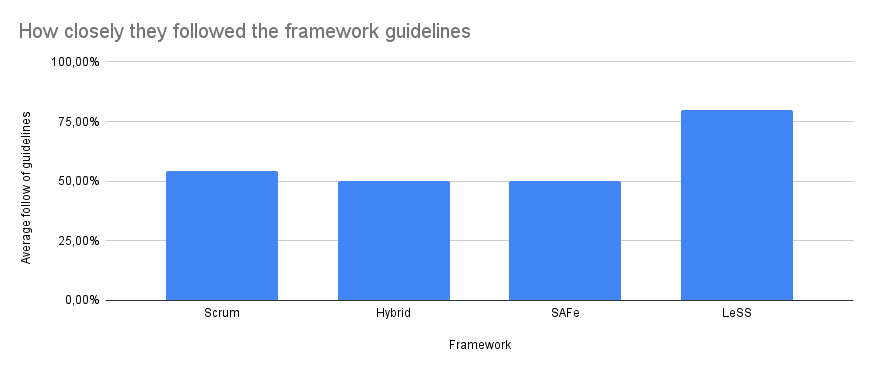
\includegraphics[width=\textwidth]{./assets/images/English/Howcloselytheyfollowedtheframeworkguidelines.png}}
        \caption{How closely they followed the framework guidelines}\label{fig:Howcloselytheyfollowedtheframeworkguidelines}
    \end{center}
\end{figure}

%\section*{Für wie gravierend halten Sie den Einfluss dieser Abweichung auf den Erfolg der Scrum Integration?}
\begin{figure}[!htb]
	\begin{center}
        \makebox[\textwidth]{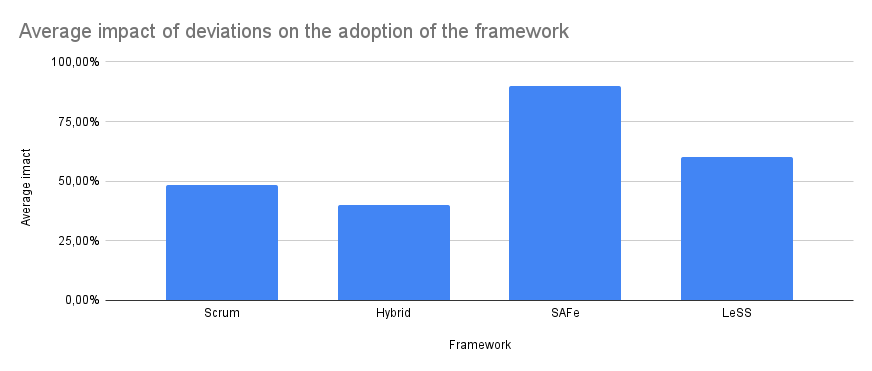
\includegraphics[width=\textwidth]{./assets/images/English/Averageimpactofdeviationsontheadoptionoftheframework.png}}
        \caption{Average impact of deviations on the adoption of the framework}\label{fig:Averageimpactofdeviationsontheadoptionoftheframework}
    \end{center}
\end{figure}

%\section*{Hatten Sie bereits Erfahrung mit einem der anderen genannten Frameworks?}
\begin{figure}[!htb]
	\begin{center}
        \makebox[\textwidth]{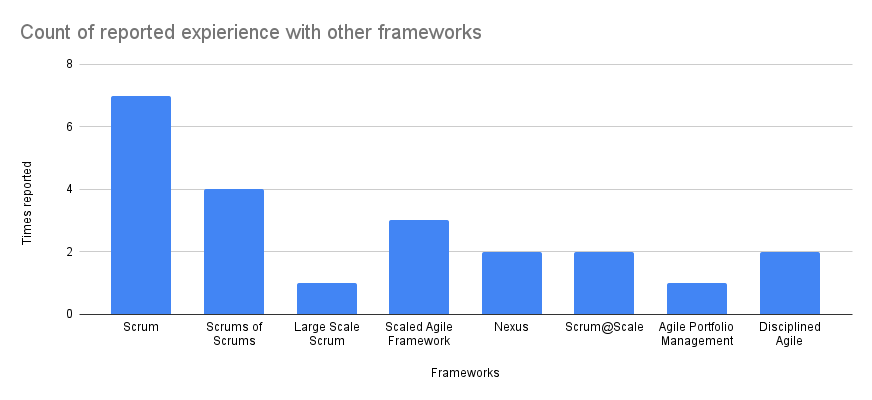
\includegraphics[width=\textwidth]{./assets/images/English/Countofreportedexpieriencewithotherframeworks.png}}
        \caption{Count of reported expierience with other frameworks}\label{fig:Countofreportedexpieriencewithotherframeworks}
    \end{center}
\end{figure}

%\section*{Welche der folgenden Methoden nutzt Ihr Unternehmen aktiv?}
\begin{figure}[!htb]
    \begin{center}
        \makebox[\textwidth]{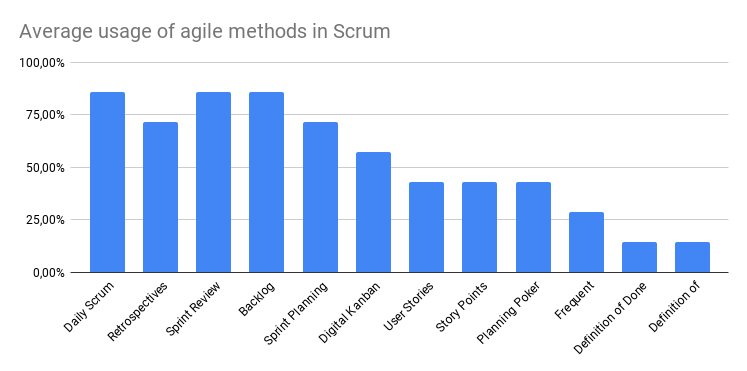
\includegraphics[width=\textwidth]{./assets/images/English/AverageusageofagilemethodsinScrum.png}}
        \caption{Average usage of agile methods in Scrum}\label{fig:AverageusageofagilemethodsinScrum}
    \end{center}
\end{figure}
\begin{figure}[!htb]
	\begin{center}
        \makebox[\textwidth]{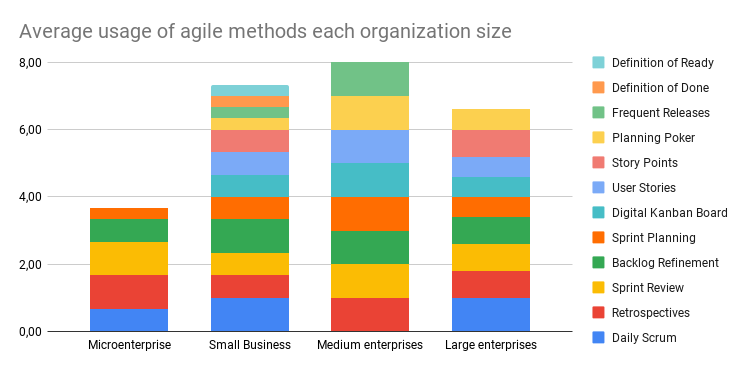
\includegraphics[width=\textwidth]{./assets/images/English/Averageusageofagilemethodseachorganizationsize.png}}
        \caption{Average usage of agile methods each organization size}\label{fig:Averageusageofagilemethodseachorganizationsize}
    \end{center}
\end{figure}
\begin{figure}[!htb]
	\begin{center}
        \makebox[\textwidth]{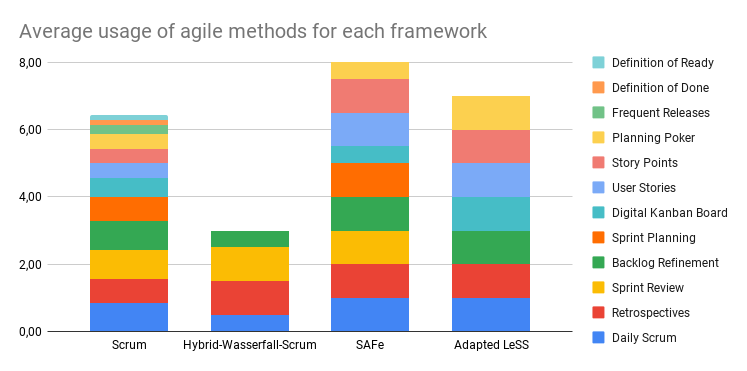
\includegraphics[width=\textwidth]{./assets/images/English/Averageusageofagilemethodsforeachframework.png}}
        \caption{Average usage of agile methods for each framework}\label{fig:Averageusageofagilemethodsforeachframework}
    \end{center}
\end{figure}

%\section*{Wie würden Sie die Expertise bewerten, die ein solches Zertifikat vermittelt?}
\begin{figure}[!htb]
    \begin{center}
        \makebox[\textwidth]{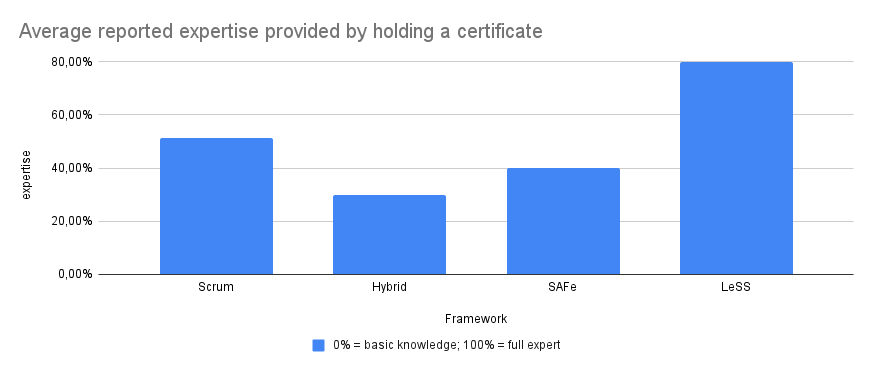
\includegraphics[width=\textwidth]{./assets/images/English/Averagereportedexpertiseprovidedbyholdingacertificate.png}}
        \caption{Average reported expertise provided by holding a certificate}\label{fig:Averagereportedexpertiseprovidedbyholdingacertificate}
    \end{center}
\end{figure}

%\section*{Wie würden Sie den Erfolg der Integration von Scrum in Ihrem Unternehmen bewerten?}
\begin{figure}[!htb]
    \begin{center}
        \makebox[\textwidth]{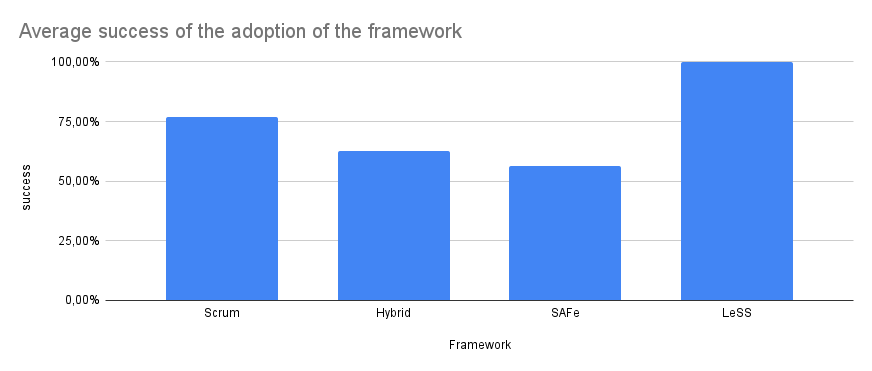
\includegraphics[width=\textwidth]{./assets/images/English/Averagesuccessoftheadoptionoftheframework.png}}
        \caption{Average success of the adoption of the framework}\label{fig:Averagesuccessoftheadoptionoftheframework}
    \end{center}
\end{figure}

%\section*{Wie schätzen Sie die Selbstorganisation und das Selbstmanagement Ihres Teams ein?}
\begin{figure}[!htb]
    \begin{center}
        \makebox[\textwidth]{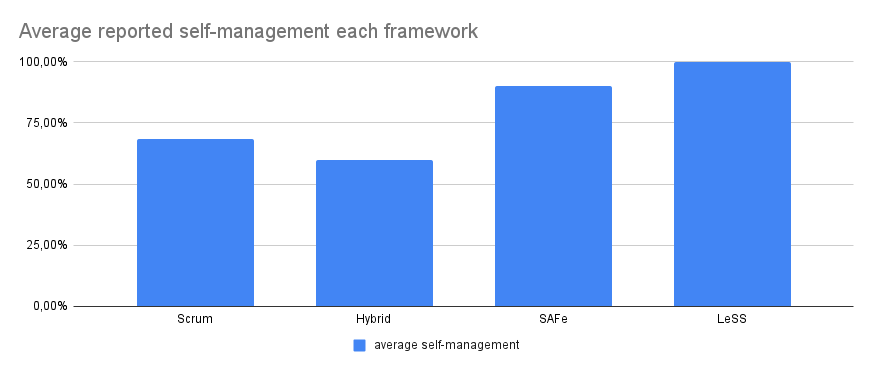
\includegraphics[width=\textwidth]{./assets/images/English/Averagereportedself-managementeachframework.png}}
        \caption{Average reported self-management each framework}\label{fig:Averagereportedself-managementeachframework}
    \end{center}
\end{figure}
\begin{figure}[!htb]
    \begin{center}
        \makebox[\textwidth]{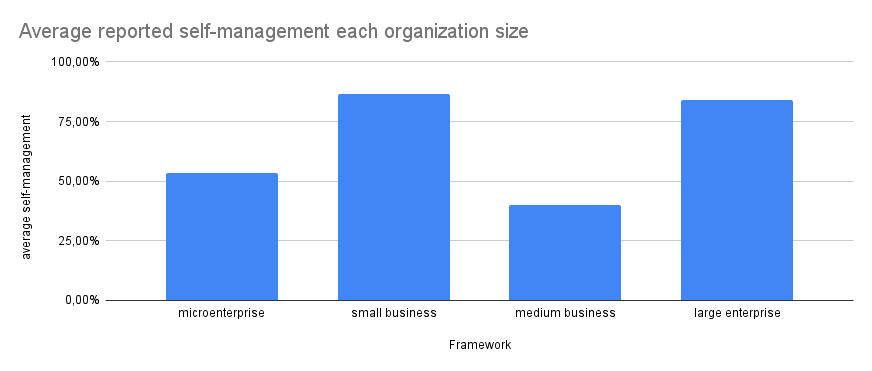
\includegraphics[width=\textwidth]{./assets/images/English/Averagereportedself-managementeachorganizationsize.png}}
        \caption{Average reported self-management each organization size}\label{fig:Averagereportedself-managementeachorganizationsize}
    \end{center}
\end{figure}

%\section*{Wie hoch ist Ihre Motivation Scrum durch ein anderes Framework zu ersetzen?}
\begin{figure}[!htb]
    \begin{center}
        \makebox[\textwidth]{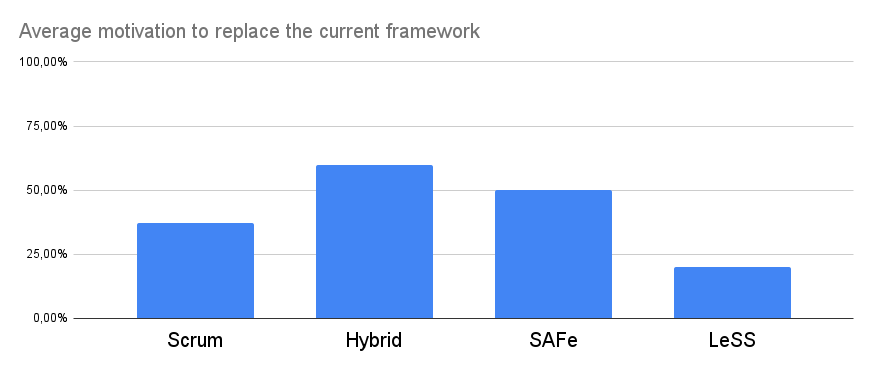
\includegraphics[width=\textwidth]{./assets/images/English/Averagemotivationtoreplacethecurrentframework.png}}
        \caption{Average motivation to replace the current framework}\label{fig:Averagemotivationtoreplacethecurrentframework}
    \end{center}
\end{figure}

%\section*{Was wären die Gründe für die Anwendung eines anderen Frameworks?}
\begin{figure}[!htb]
    \begin{center}
        \makebox[\textwidth]{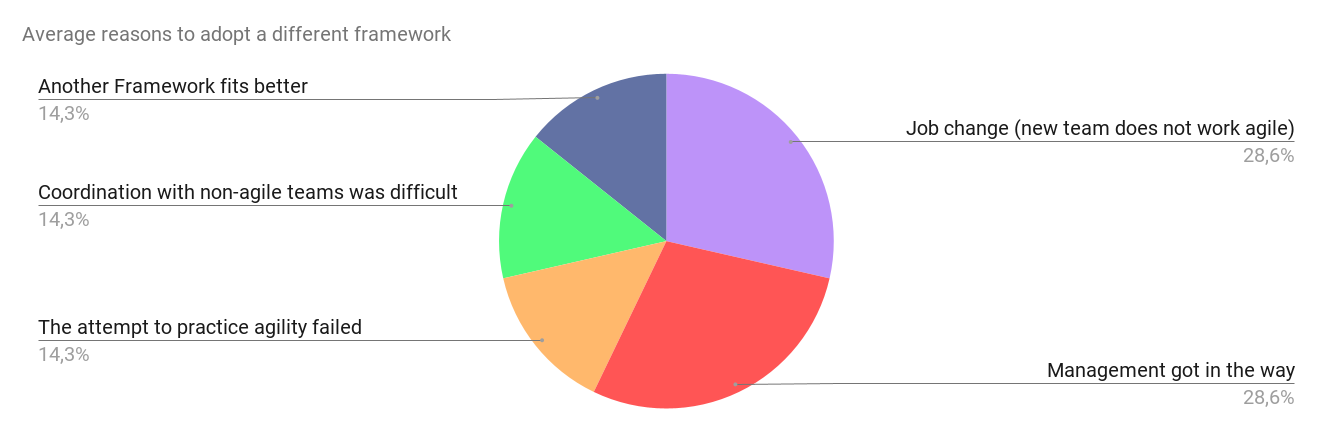
\includegraphics[width=\textwidth]{./assets/images/English/Averagereasonstoadoptadifferentframework.png}}
        \caption{Average reasons to adopt a different framework}\label{fig:Averagereasonstoadoptadifferentframework}
    \end{center}
\end{figure}

%\section*{Welche der folgenden Gründe waren es, die zur Integration von Scrum in Ihrem Unternehmen gesorgt haben?}
\begin{figure}[!htb]
    \begin{center}
        \makebox[\textwidth]{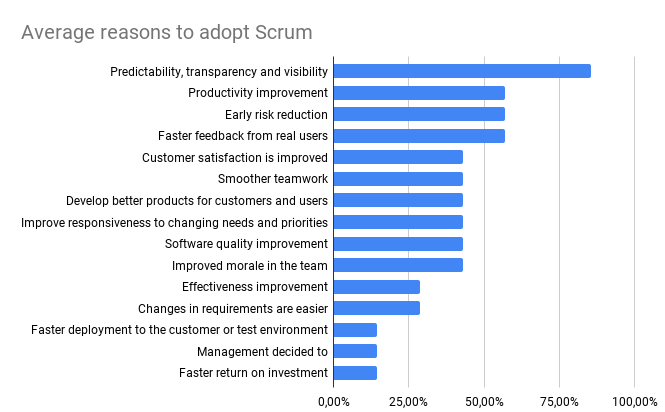
\includegraphics[width=\textwidth]{./assets/images/English/AveragereasonstoadoptScrum.png}}
        \caption{Average reasons to adopt Scrum}\label{fig:AveragereasonstoadoptScrum}
    \end{center}
\end{figure}

%\section*{Welche der folgenden Herausforderungen hatte Ihr Unternehmen bei der Integration von Scrum?}
\begin{figure}[!htb]
    \begin{center}
        \makebox[\textwidth]{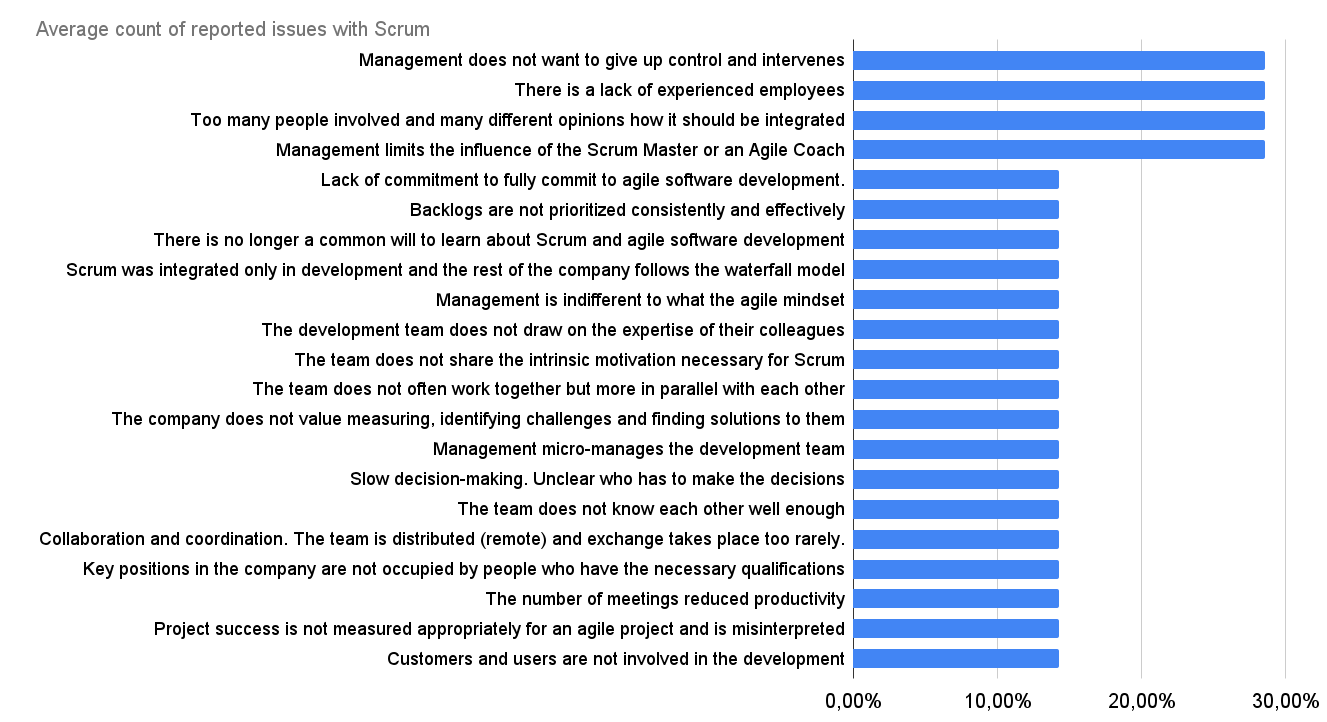
\includegraphics[width=\textwidth]{./assets/images/English/AveragecountofreportedissueswithScrum.png}}
        \caption{Average count of reported issues with Scrum}\label{fig:AveragecountofreportedissueswithScrum}
    \end{center}
\end{figure}
\begin{figure}[!htb]
    \begin{center}
        \makebox[\textwidth]{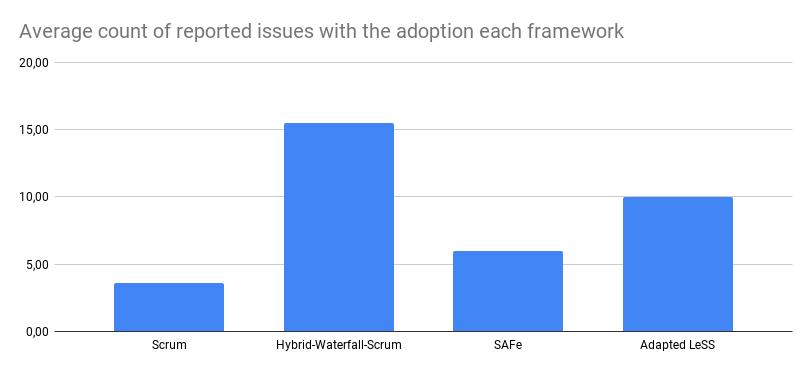
\includegraphics[width=\textwidth]{./assets/images/English/Averagecountofreportedissueswiththeadoptioneachframework.png}}
        \caption{Average count of reported issues with the adoption each framework}\label{fig:Averagecountofreportedissueswiththeadoptioneachframework}
    \end{center}
\end{figure}
\begin{figure}[!htb]
    \begin{center}
        \makebox[\textwidth]{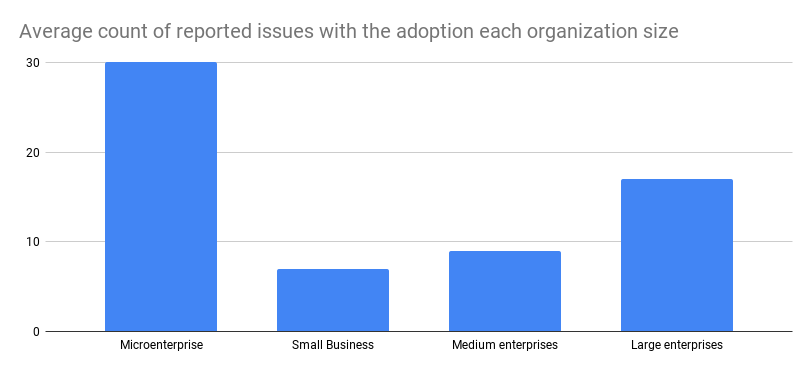
\includegraphics[width=\textwidth]{./assets/images/English/Averagecountofreportedissueswiththeadoptioneachorganizationsize.png}}
        \caption{Average count of reported issues with the adoption each organization size}\label{fig:Averagecountofreportedissueswiththeadoptioneachorganizationsize}
    \end{center}
\end{figure}

%\section*{Welche der folgenden Lösungsansätze hatte auch Ihr Unternehmen versucht?}
\begin{figure}[!htb]
    \begin{center}
        \makebox[\textwidth]{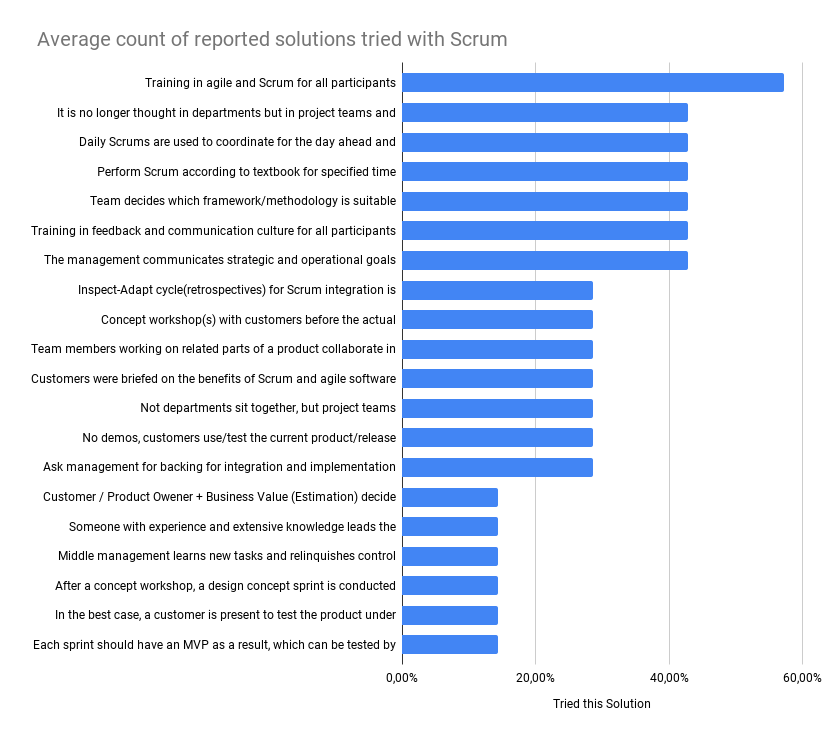
\includegraphics[width=\textwidth]{./assets/images/English/AveragecountofreportedsolutionstriedwithScrum.png}}
        \caption{Average count of reported solutions tried with Scrum}\label{fig:AveragecountofreportedsolutionstriedwithScrum}
    \end{center}
\end{figure}
\begin{figure}[!htb]
    \begin{center}
        \makebox[\textwidth]{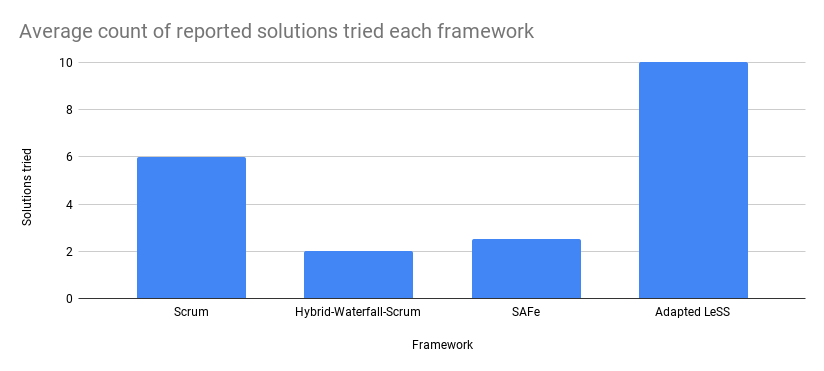
\includegraphics[width=\textwidth]{./assets/images/English/Averagecountofreportedsolutionstriedeachframework.png}}
        \caption{Average count of reported solutions tried each framework}\label{fig:Averagecountofreportedsolutionstriedeachframework}
    \end{center}
\end{figure}
\begin{figure}[!htb]
    \begin{center}
        \makebox[\textwidth]{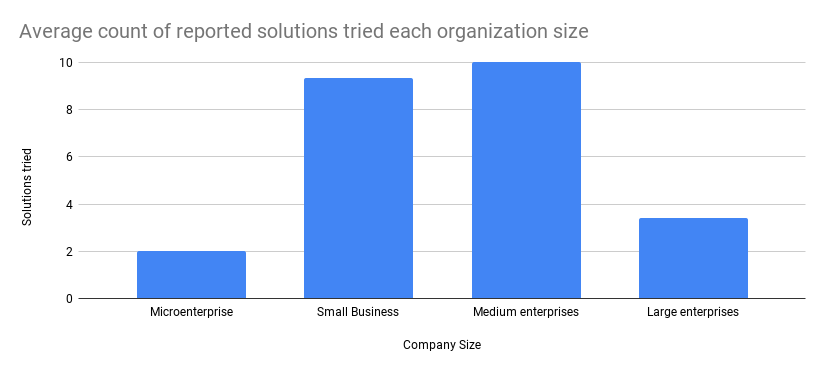
\includegraphics[width=\textwidth]{./assets/images/English/Averagecountofreportedsolutionstriedeachorganizationsize.png}}
        \caption{Average count of reported solutions tried each organization size}\label{fig:Averagecountofreportedsolutionstriedeachorganizationsize}
    \end{center}
\end{figure}

%\section*{Welche Folgen von agiler Transformation treffen auf Ihr Unternehmen zu?}
\begin{figure}[!htb]
    \begin{center}
        \makebox[\textwidth]{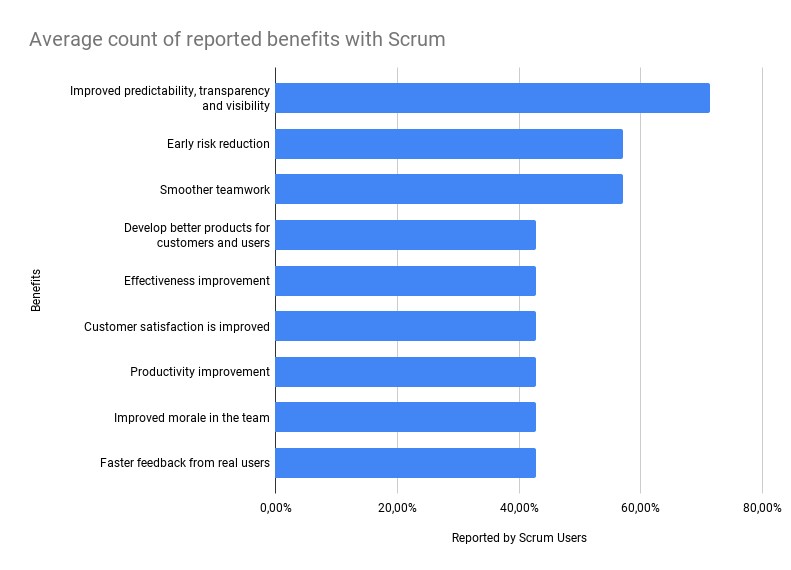
\includegraphics[width=\textwidth]{./assets/images/English/AveragecountofreportedbenefitswithScrum.png}}
        \caption{Average count of reported benefits with Scrum}\label{fig:AveragecountofreportedbenefitswithScrum}
    \end{center}
\end{figure}
\begin{figure}[!htb]
    \begin{center}
        \makebox[\textwidth]{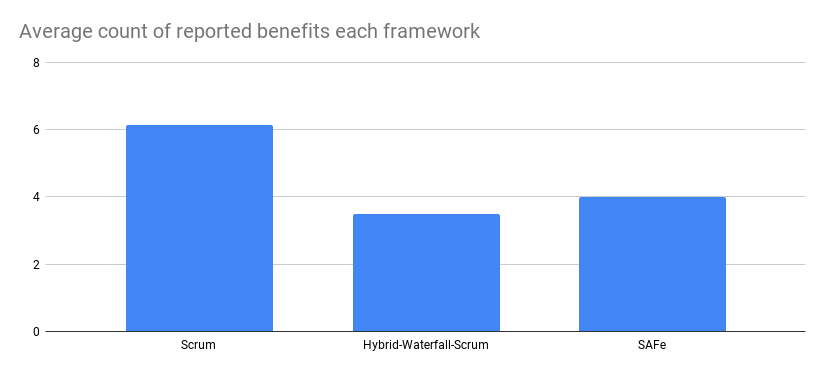
\includegraphics[width=\textwidth]{./assets/images/English/Averagecountofreportedbenefitseachframework.png}}
        \caption{Average count of reported benefits each framework}\label{fig:Averagecountofreportedbenefitseachframework}
    \end{center}
\end{figure}
\begin{figure}[!htb]
    \begin{center}
        \makebox[\textwidth]{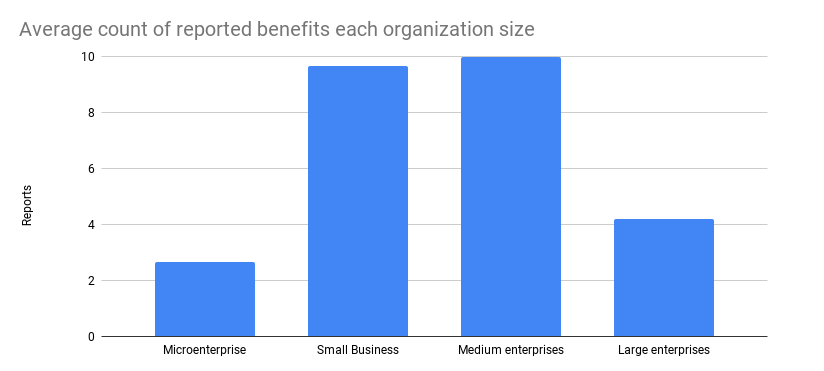
\includegraphics[width=\textwidth]{./assets/images/English/Averagecountofreportedbenefitseachorganizationsize.png}}
        \caption{Average count of reported benefits each organization size}\label{fig:Averagecountofreportedbenefitseachorganizationsize}
    \end{center}
\end{figure}



\newpage
\phantomsection%
%----------------------------------------------------------------------------------------
%	Affidavit
%----------------------------------------------------------------------------------------
%!TEX root = ../mai-joel_maximilian-bachelor_thesis.tex
%----------------------------------------------------------------------------------------
%	Debug options
%----------------------------------------------------------------------------------------
% chktex-file 2
% chktex-file 8
% chktex-file 11
% chktex-file 13
% chktex-file 18
% chktex-file 36
% chktex-file 39
% chktex-file 44
%----------------------------------------------------------------------------------------
\addcontentsline{toc}{chapter}{Affidavit}
\chapter*{Eidesstattliche Erklärung}

Ich versichere, die von mir vorgelegte Arbeit selbständig verfasst zu haben.\newline
Alle Stellen, die wörtlich oder sinngemäß aus veröffentlichten oder nicht veröffentlichten Arbeiten anderer entnommen sind, habe ich als entnommen kenntlich gemacht. Sämtliche Quellen und Hilfsmittel, die ich für die Arbeit benutzt habe, sind angegeben.\newline
Die Arbeit hat mit gleichem Inhalt bzw. in wesentlichen Teilen noch keiner anderen Prüfungsbehörde vorgelegen.
\vspace{1.5cm}

Gummersbach, Freitag 17. Februar 2023
\vspace{1cm}

%----------------------------------------------------------------------------------------
%	Insert Signature as Image here
%----------------------------------------------------------------------------------------
\begin{figure}[!ht]
	
\includegraphics[width=0.26\textwidth]{assets/images/mySignature.jpg}
\end{figure}

Joël Maximilian Mai
\newpage
\newpage

\end{document}
